\documentclass[cjk]{beamer}
\mode<presentation>{
  %\usetheme{Warsaw}
  \usetheme{CambridgeUS}
  \usecolortheme{beaver}
  \setbeamercovered{transparent}
}
%% \usepackage[T1]{fontenc} % Needed for Type1 Concrete
%% %% \usepackage{concrete} % Loads Concrete + Euler VM
%% %% \usepackage{pxfonts} % Or palatino or mathpazo
%% \usepackage{eulervm} %
%% %% \usepackage{kerkis} % Kerkis roman and sans
%% %% \usepackage{kmath} % Kerkis math
%% \usepackage{fourier}
\usepackage{pgf}
\usepackage{tikz}
\usetikzlibrary{calc}
\usetikzlibrary{arrows,snakes,backgrounds,shapes}
\usetikzlibrary{matrix,fit,positioning,decorations.pathmorphing}
\usepackage{CJK} 
\usepackage{amsmath,amssymb,amsfonts}
\usepackage{mathdots}
\usepackage{subfigure}
\usepackage{caption}
\usepackage{verbatim,color,xcolor}
\usepackage{graphicx}
\usepackage{manfnt}
\usepackage{fancybox}
\usepackage{textcomp}
\usepackage{multirow,multicol}
\usepackage{parcolumns}
\usepackage{framed}
\usepackage{threeparttable}
\usepackage{extarrows}
\usepackage{listings}
\lstset{
  keywordstyle=\color{blue!70},
  frame=lines,
  basicstyle=\ttfamily\small,
  commentstyle=\small\color{red},
  rulesepcolor=\color{red!20!green!20!blue!20},
  tabsize=4,
  numbersep=5pt,
  backgroundcolor=\color[rgb]{0.95,1.0,1.0},
  showspaces=false,
  showtabs=false,
  extendedchars=false,
  escapeinside=``
}
%% \usepackage[utf8]{inputenc}
%% \usepackage[upright]{fourier}   %

% ######### DEFINE COLOR ###############
\definecolor{blue}{rgb}{0.0,0.0,1.0}
\definecolor{red}{rgb}{1.0,0.0,0.0}
%\definecolor{purple}{rgb}{1.0,0.0,0.0}
\definecolor{electricpurple}{rgb}{0.75, 0.0, 1.0}

%%%% \renewcommand *****
\renewcommand{\lstlistingname}{}
\newcommand{\tf}{\ttfamily}
\newcommand{\ttt}{\texttt}
\newcommand{\blue}{\textcolor{blue}}
\newcommand{\red}{\textcolor{red}}
\newcommand{\purple}{\textcolor{purple}}
\newcommand{\ft}{\frametitle}
\newcommand{\bs}{\boldsymbol}
\newcommand{\disp}{\displaystyle}
\newcommand{\ds}{\displaystyle}
\newcommand{\vd}{\vdots}
\newcommand{\cd}{\cdots}
\newcommand{\dd}{\ddots}
\newcommand{\id}{\iddots}
\newcommand{\XX}{\mathbf{X}}
\newcommand{\PP}{\mathbf{P}}
\newcommand{\QQ}{\mathbf{Q}}
\newcommand{\xx}{\mathbf{x}}
\newcommand{\yy}{\mathbf{y}}
\newcommand{\bb}{\mathbf{b}}
\newcommand{\aaa}{\mathbf{a}}
\newcommand{\A}{\mathbf{A}}
\newcommand{\B}{\mathbf{B}}
\newcommand{\C}{\mathbf{C}}
\newcommand{\D}{\mathbf{D}}
\newcommand{\E}{\mathbf{E}}
\newcommand{\U}{\mathbf{U}}
\newcommand{\X}{\mathbf{X}}
\newcommand{\Y}{\mathbf{Y}}
\newcommand{\Z}{\mathbf{Z}}
\newcommand{\T}{\mathbf{T}}
\newcommand{\zero}{\mathbf{0}}
\newcommand{\II}{\mathbf{I}}
\newcommand{\ii}{\mathbf{i}}
\newcommand{\jj}{\mathbf{j}}
\newcommand{\kk}{\mathbf{k}}
\newcommand{\uu}{\mathbf{u}}
\newcommand{\vv}{\mathbf{v}}
\newcommand{\ee}{\mathbf{e}}
\newcommand{\Lambdabd}{\mathbf{\Lambda}}
\newcommand{\alphabd}{\boldsymbol{\alpha}}
\newcommand{\betabd}{\boldsymbol{\beta}}
\newcommand{\gammabd}{\boldsymbol{\gamma}}
\newcommand{\xibd}{\boldsymbol{\xi}}
\newcommand{\epsilonbd}{\boldsymbol{\epsilon}}
\newcommand{\etabd}{\boldsymbol{\eta}}
\newcommand{\rr}{\mathrm{r}}
\newcommand{\RR}{\mathrm{R}}
\newcommand{\RRR}{\mathbb{R}}
\newcommand{\CCC}{\mathbb{C}}




\begin{document}
\begin{CJK}{UTF8}{gkai} 
  \CJKtilde
  \renewcommand{\proofname}{\vspace{0.2cm}\textbf{证明: \ }}
  \newcommand{\jiename}{\vspace{0.2cm}\textbf{解: \ }}
  \title{线性代数}
\subtitle{总复习}
\institute[]{
  
\includegraphics[width=0.5in]{wuda_log.pdf} \\
  数学与统计学院 \\
  Email: ~~ xpzhang.math@whu.edu.cn    \\
  Homepage: ~~http://staff.whu.edu.cn/show.jsp?n=Zhang\%20Xiaoping
}

\author{张晓平}
\date{}
\subject{线性代数}
% 如果你想插入学校的徽章, 其文件名为 "university-logo-filename.xxx", 
% 其中 xxx 是 pdflatex 能接受的格式, 则可用以下命令插入
%% \pgfdeclareimage[height=0.5cm]{wuda}{wudalogo.pdf}
%% \logo{\pgfuseimage{wuda}}
%% \pgfdeclareimage[width=1.0cm]{university-logo}{university-logo-filename.jpg}
%% \logo{\pgfuseimage{university-logo}}

% 如果你想要在每一小节之前都显示一下目录, 则可把一下小段的注解号 "%" 删去
%% \AtBeginSubsection[]
%% {
%%  \begin{frame}<beamer>
%%    \frametitle{概要}
%%    \tableofcontents[currentsection,currentsubsection]
%%  \end{frame}
%% }

%除掉以下命令的注解 "%" 后, 许多环境都会自动逐段显示
% \beamerdefaultoverlayspecification{<+->}

%% 的演示文稿仅供参考, 不过可以提供一些忠告:
% - 除总结外, 最好不超过 3 节;
% - 每节至多分成 3 小节;
% - 每屏约 30 秒至 2 分钟, 因此总共 15 至 30 屏为佳.
% - 一般说来, 会议听众对你所报告的东西知之甚少, 因此尽量简单!
% - 在 20 分钟报告里只要讲清主要思想即可, 不要深入细节, 宁可牺牲一点严格性;
% - 如果你略去了证明或实现的关键细节, 只要声明一下即可, 没有人会感到不高兴.

  
  
  \begin{frame}
    \titlepage
  \end{frame}

  \begin{frame}
    \frametitle{目录}
    \tableofcontents[currentsection]
  \end{frame}

  \AtBeginSection[]{
    \begin{frame}[allowframebreaks]
      \tableofcontents[currentsection]%,hideallsubsections]
    \end{frame}
  }
  \AtBeginSubsection[]{
    \begin{frame}[shrink]
      \tableofcontents[sectionstyle=show/shaded,subsectionstyle=show/shaded/hide]
    \end{frame}
  }

   \section{行列式简介}

\begin{frame}

  行列式出现于线性方程组的求解,它最早是一种速记的表达式,现在已经是数学中一种非常有用的工具。\\

  \pause
  \begin{itemize}
  \item 行列式是由莱布尼茨和日本数学家关孝和分别发明的。 \\ 
    \begin{itemize}
    \item 1683年,日本数学家关孝和在其著作《解伏题之法》中也提出了行列式的概念与算法。《解伏题之法》的意思就是“解行列式问题的方法”,书里对行列式的概念和它的展开已经有了清楚的叙述。\\[0.1in]
    \item 1693年4月,莱布尼茨在写给洛比达的一封信中使用并给出了行列式,并给出方程组的系数行列式为零的条件。

    \end{itemize}
    \pause 
  \item
    1750年,瑞士数学家克莱姆在其著作《线性代数分析导引》中,对行列式的定义和展开法则给出了比较完整、明确的阐述,并给出了现在我们所称的解线性方程组的克莱姆法则。
  \end{itemize}
    
\end{frame}

\begin{frame}
  \begin{itemize}

  \item
    在行列式的发展史上,第一个对行列式理论做出连贯的逻辑的阐述,即把行列式理论与线性方程组求解相分离的人,是法国数学家范德蒙。
    范德蒙自幼在父亲的指导下学习音乐,但对数学有深厚的兴趣,后来终于成为法兰西科学院院士。他给出了用二阶子式和它们的余子式来展开行列式的法则,就对行列式本身这一点来说,他是这门理论的奠基人。
    \\[0.1in] \pause
  \item
    1772年,拉普拉斯在一篇论文中证明了范德蒙提出的一些规则,推广了他的展开行列式的方法。\\[0.1in]
    \pause
  \item
    继范德蒙之后,在行列式的理论方面,又一位做出贡献的就是另一位法国大数学家柯西。1815年,柯西在一篇论文中给出了行列式的第一个系统的、几乎是近代的处理。其中主要结果之一是行列式的乘法定理。另外,他第一个把行列式的元素排成方阵,采用双足标记法;引进了行列式特征方程的术语;给出了相似行列式的概念;改进了拉普拉斯的行列式展开定理并给出了一个证明等。
  \end{itemize}

  
\end{frame}


   %%%%%m
\section{行列式的定义}
\subsection{二阶行列式}
%%%%%

\begin{frame}
    \begin{exampleblock}{引例}
      用消元法求解
      $$
      \left \lbrace
      \begin{array}{l}
        a_{11} x_1 + a_{12} x_2 = b_1, \\[0.2cm]
        a_{21} x_1 + a_{22} x_2 = b_2.
      \end{array}
      \right.
      $$
    \end{exampleblock}
    \pause 
    消去$x_2$得
    $$
    (a_{11}a_{22}-a_{12}a_{21})x_1 = b_1 a_{22} - b_2 a_{12},
    $$
    消去$x_1$得
    $$
    (a_{11}a_{22}-a_{12}a_{21})x_2 = b_2 a_{11} - b_1 a_{11}.
    $$
    \pause
    
    若$\boxed{\red{a_{11}a_{22}-a_{12}a_{21}\ne0}}$,则
    $$
    x_1 = \frac{b_1 a_{22} - b_2 a_{12}}{a_{11}a_{22}-a_{12}a_{21}}, \ \
    x_2 = \frac{b_2 a_{11} - b_1 a_{11}}{a_{11}a_{22}-a_{12}a_{21}}.
    $$
\end{frame}

\begin{frame}

    %%%%
    \begin{block}{二阶行列式}
      由$2^2=4$个数,按下列形式排成2行2列的方形
      $$
      \left|
      \begin{array}{cc}
        a_{11} & a_{12} \\[0.2cm]
        a_{21} & a_{22} 
      \end{array}
      \right|,
      $$
      其被定义成一个数
      $$
      \left|
      \begin{array}{cc}
        a_{11} & a_{12} \\[0.2cm]
        a_{21} & a_{22} 
      \end{array}
      \right| = a_{11}a_{22} - a_{12}a_{21} \equiv D,
      $$
      该数称为由这四个数构成的二阶行列式。
    \end{block}

\end{frame}

\begin{frame}

    %%%%
    \begin{itemize}
    \item 
      $\red{a_{ij}}$表示行列式的元素。\\[0.2cm]
      $i$为行标,表明该元素位于第$i$行;\\[0.2cm]
      $j$为列标,表明该元素位于第$j$列。\\[0.4cm]
    \item
      对角线法则\\
      \begin{center}
        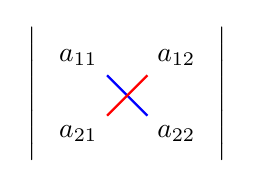
\begin{tikzpicture}
          \matrix (A) [matrix of nodes,ampersand replacement=\&,row sep=15pt,column sep=15pt,left delimiter=|,
          right delimiter=|] {
            $a_{11}$ \& $a_{12}$  \\
            $a_{21}$ \& $a_{22}$  \\
          };
          \draw[blue, thick] (A-1-1.south east) -- (A-2-2.north west);
          \draw[red,  thick] (A-1-2.south west) -- (A-2-1.north east);
        \end{tikzpicture}
      \end{center}
    \end{itemize}
\end{frame}

\begin{frame}

    %%%%%%
    \begin{itemize}
    \item 
      类似地,
      $$
      \begin{array}{l}
        b_1 a_{22} - b_2 a_{12} = \left|
        \begin{array}{cc}
          b_1 & a_{12} \\
          b_2 & a_{22} 
        \end{array}
        \right|  \equiv D_1\\[0.4cm]
        b_2 a_{11} - b_1 a_{21} = \left|
        \begin{array}{cc}
          a_{11} & b_1 \\
          a_{21} & b_2
        \end{array}
        \right|  \equiv D_2\\
      \end{array}
      $$      
      则上述方程组的解可表示为
      $$
      x_1 = \frac{D_1}{D},\ \
      x_2 = \frac{D_2}{D}.
      $$
    \end{itemize}


\end{frame}


\begin{frame}
  
    \uncover<1->{
      \begin{block}{例1}
        求解二元线性方程组
        $$
        \left\{
        \begin{array}{l}
          3x_1 - 2x_2 = 12, \\[0.2cm]
          2x_1 + x_2  = 1.
        \end{array}
        \right.
        $$
      \end{block}
    }
    \uncover<2->{
      解:因为
      $$
      \begin{array}{l}
        D = \left|
        \begin{array}{cc}
          3 & -2 \\
          2 & 1 
        \end{array}
        \right| = 7 \ne 0,\\[0.4cm]
        D_1 = \left|
        \begin{array}{cc}
          12 & -2 \\
          1 & 1 
        \end{array}
        \right| = 14 , \\[0.4cm]
        D_2 = \left|
        \begin{array}{cc}
          3 & 12 \\
          2 & 1 
        \end{array}
        \right| = -21,
      \end{array}
      $$
      因此,
      $$
      x_1=\frac{D_1}{D}=2, \ \ x_2 = \frac{D_2}{D} = -3.
      $$
    }

\end{frame}

\subsection{三阶行列式}
%%%%%

\begin{frame}

  
  \begin{overprint}
    %%%%
    \onslide<1>
    \begin{block}{三阶行列式}
      由$3^2=9$个数组成的3行3列的三阶行列式,则按如下形式定义一个数
      $$ 
      D_3 = 
      \left|
      \begin{array}{ccc}
        a_{11} & a_{12} & a_{13} \\[0.2cm]
        a_{21} & a_{22} & a_{23} \\[0.2cm]
        a_{31} & a_{32} & a_{33} 
      \end{array}
      \right|
      = 
      \begin{array}{l}
          a_{11}a_{22}a_{33} + a_{12}a_{23}a_{31} + a_{13}a_{21}a_{32} \\[0.2cm]
        - a_{13}a_{22}a_{31} - a_{11}a_{23}a_{32} - a_{12}a_{21}a_{33}
      \end{array}
      $$

    \end{block}
  \end{overprint}
\end{frame}



\begin{frame}
 
    \begin{itemize}
    \item
      沙路法\\

       
              \begin{tikzpicture}               
                
                \only<1->{
                   \matrix(A) [matrix of math nodes,nodes in empty cells,ampersand replacement=\&,row sep=15pt,column sep=15pt] {
                       \&  a_{11} \& a_{12} \& a_{13}  \& \red{a_{11}} \& \red{a_{12}} \&\\
                       \&  a_{21} \& a_{22} \& a_{23}  \& \red{a_{21}} \& \red{a_{22}} \&\\
                       \&  a_{31} \& a_{32} \& a_{33}  \& \red{a_{31}} \& \red{a_{32}} \&\\
                   -   \&    -        \&   -        \&               \&   +         \&   +        \& +\\
                };
                }
                \only<2->{
                 \draw[blue,thick] (A-1-2.center) -- (A-4-5.center);
                 \draw[blue,thick] (A-1-3.center)  -- (A-4-6.center);
                 \draw[blue,thick] (A-1-4.center) -- (A-4-7.center); 
                }
                \only<3->{
                 \draw[red,thick,->] (A-1-6.center) -- (A-4-3.center);
                 \draw[red,thick,->] (A-1-5.center) -- (A-4-2.center);
                 \draw[red,thick,->] (A-1-4.center) -- (A-4-1.center); 
                }

              \end{tikzpicture}          
    \end{itemize}
\end{frame}


\begin{frame}
  \uncover<1->{
    \begin{block}{例3}
      计算
      $$
      D_3 = 
      \left |
      \begin{array}{ccc}
        1  & 2 & -4 \\ 
        -2 & 2 & 1  \\
        -3 & 4 & -2
      \end{array}
      \right|
      $$
    \end{block}
  }
  \uncover<2->{
    解:由对角线法则可知,
    $$
    \begin{array}{ll}
      D_3 &=   1\times   2  \times (-2) +   2  \times 1 \times (-3) + (-2) \times 4 \times (-4)\\[0.2cm]
      & - 2\times (-2) \times (-2) - (-4) \times 2 \times (-3) +   1  \times 1 \times   4\\[0.2cm]
      & = -14.
    \end{array}
    $$
  }
\end{frame}


\begin{frame}
  \uncover<1->{
    \begin{block}{例3}
      求方程
      $$
      \left |
      \begin{array}{ccc}
        1  & 1 & 1 \\
        2  & 3 & x  \\
        4  & 9 & x^2
      \end{array}
      \right| = 0
      $$      
    \end{block}
  }
  \uncover<2->{
    解:行列式
    $$ 
    D = 3x^2 + 18 + 4x - 2x^2 - 12 - 9x 
    = x^2 - 5x + 6
    $$
    由此可知$x=2$或$3$。
  }
\end{frame}


\begin{frame}
  如果三元一次方程组
  $$
  \begin{array}{c}  
    a_{11}x_1 + a_{12}x_2 + a_{13}x_3 = b_1, \\
    a_{21}x_1 + a_{22}x_2 + a_{23}x_3 = b_2, \\
    a_{31}x_1 + a_{32}x_2 + a_{33}x_3 = b_3,
  \end{array}
  $$
  的系数行列式
  $$
  D = \left|
  \begin{array}{ccc}
    a_{11} & a_{12} & a_{13}\\
    a_{21} & a_{22} & a_{23}\\
    a_{31} & a_{32} & a_{33}
  \end{array}
  \right| \ne 0
  $$
  则用消元法求解可得
  $$
  x_1 = \frac{D_1}{D}, \quad
  x_2 = \frac{D_2}{D}, \quad
  x_3 = \frac{D_3}{D}, \quad
  $$
  其中
  $$
  D_1 = \left|
  \begin{array}{ccc}
    b_1 & a_{12} & a_{13}\\
    b_2 & a_{22} & a_{23}\\
    b_3 & a_{32} & a_{33}
  \end{array}
  \right|, \
  D_2 = \left|
  \begin{array}{ccc}
    a_{11} & b_1 & a_{13}\\
    a_{21} & b_2 & a_{23}\\
    a_{31} & b_3 & a_{33}
  \end{array}
  \right|, \
  D_3= \left|
  \begin{array}{ccc}
    a_{11} & a_{12} & b_1 \\
    a_{21} & a_{22} & b_2 \\
    a_{31} & a_{32} & b_3 
  \end{array}
  \right|.
  $$

\end{frame}


\begin{frame}
  从二、三阶行列式的展开式中可发现:
  $$
  \begin{array}{l}
    D  =  \left|
    \begin{array}{ccc}
      a_{11} & a_{12} & a_{13}\\
      a_{21} & a_{22} & a_{23}\\
      a_{31} & a_{32} & a_{33}
    \end{array}
    \right| \\[0.6cm]
     = 
    a_{11}a_{22}a_{33}+a_{12}a_{23}a_{31}+a_{13}a_{21}a_{32}
    -a_{13}a_{22}a_{31}-a_{12}a_{21}a_{33}-a_{11}a_{23}a_{32} \\[0.3cm]\pause 
     = 
    a_{11}(a_{22}a_{33}-a_{23}a_{32})-
    a_{12}(a_{21}a_{33}-a_{23}a_{31})+
    a_{13}(a_{21}a_{32}-a_{22}a_{31}) \\[0.3cm] \pause 
     = 
    a_{11} \underbrace{\left| \begin{array}{ccc} a_{22} & a_{33} \\ a_{23} & a_{32} \end{array} \right|}_{M_{11}} -
    a_{12} \underbrace{\left| \begin{array}{ccc} a_{21} & a_{23} \\ a_{31} & a_{33} \end{array} \right|}_{M_{12}} +
    a_{13} \underbrace{\left| \begin{array}{ccc} a_{21} & a_{22} \\ a_{31} & a_{32} \end{array} \right|}_{M_{13}}
  \end{array}
  $$
  \pause 
  这里,$M_{11},M_{12},M_{13}$分别称为$a_{11},a_{12},a_{13}$的\red{余子式},并称
  $$
  A_{11} = (-1)^{1+1} M_{11}, \quad
  A_{12} = (-1)^{1+2} M_{12}, \quad
  A_{13} = (-1)^{1+3} M_{13}
  $$
  分别称为$a_{11},a_{12},a_{13}$的\red{代数余子式}。\pause 这样,$D$可表示为
  $$
  D= a_{11}A_{11} + a_{11}A_{13} + a_{13}A_{13}.
  $$
\end{frame}


\begin{frame}
  同样地,
  $$
  D = \left| \begin{array}{ccc} a_{11} & a_{12} \\ a_{21} & a_{22} \end{array} \right|
  = a_{11} A_{11} + a_{12} A_{12},
  $$
  其中
  $$
  A_{11} = (-1)^{1+1}|a_{22}| =  a_{22},\quad
  A_{11} = (-1)^{1+2}|a_{21}| = -a_{21}.
  $$
  \pause 
  注意这里的$|a_{22}|,~|a_{21}|$是一阶行列式,而不是绝对值。

  \pause 
  \vspace{0.1in}
  \red{我们把一阶行列式$|a|$定义为$a$。}

\end{frame}

\subsection{$n$阶行列式的定义}

\begin{frame}
  \begin{block}{定义}
    由$n^2$个数$a_{ij}(i,j=1,2,\cdots,n)$组成的$n$阶行列式
    \begin{equation}\label{Dn}
      D = \left|
      \begin{array}{cccc}
        a_{11}  &  a_{12} & \cdots & a_{1n} \\
        a_{21}  &  a_{22} & \cdots & a_{2n} \\
        \vdots & \vdots & \ddots & \vdots\\  
        a_{n1}  &  a_{n2} & \cdots & a_{nn} 
      \end{array}
      \right|
    \end{equation}
    是一个数。
  \end{block}
\end{frame}

\begin{frame}
  \begin{block}{定义(续)}
    \begin{itemize}
    \item 当$n=1$时,定义$D=|a_{11}|=a_{11}$;\pause 
    \item 当$n\ge2$时,定义
      \begin{equation}
        D = a_{11} A_{11} + a_{12} A_{12} + \cdots + a_{1n} A_{1n},
      \end{equation}
      其中
      $$A_{1j} = (-1)^{1+j} M_{1j}$$
      而$M_{1j}$是$D$中划去第$1$行第$j$列后,按原顺序排成的$n-1$阶行列式,即
      $$
      M_{1j} =   \left|
      \begin{array}{cccccc}
        a_{21}  & \cdots&  a_{2,j-1}  &  a_{2,j+1}  & \cdots & a_{2n} \\
        a_{31}  & \cdots&  a_{3,j-1}  &  a_{3,j+1}  & \cdots & a_{3n} \\
        \vdots &       &  \vdots &  \vdots &  & \vdots\\  
        a_{n1}  & \cdots&  a_{n,j-1}  &  a_{n,j+1}  & \cdots & a_{nn} 
      \end{array}
      \right| \quad (j = 1,2,\cdots, n),
      $$
      并称$M_{1j}$为$a_{1j}$的余子式,$A_{1j}$为$a_{1j}$的代数余子式.
    \end{itemize}
  \end{block}

\end{frame}



\begin{frame}

  \begin{block}{注}
    \begin{enumerate}
    \item[1]
      在$D$中,$a_{11},a_{22},\cdots,a_{nn}$所在的对角线称为行列式的\red{主对角线},$a_{11},a_{22},\cdots,a_{nn}$称为\red{主对角元}。\\[0.1in]
    \item[2]
      行列式$D$是由$n^2$个元素构成的$n$次齐次多项式:\\[0.1in]
      \begin{itemize}
      \item 二阶行列式的展开式有$2!$项 \\[0.1in]
      \item 三阶行列式的展开式有$3!$项 \\[0.1in]
      \item $n$阶行列式的展开式有$n!$项,其中每一项都是不同行不同列的$n$个元素的乘积,带正号的项与带负号的项各占一半。
      \end{itemize}

    \end{enumerate}
    
  \end{block}
\end{frame}


\begin{frame}
  \begin{exampleblock}{例}
    证明:$n$阶下三角行列式
    $$
    D_n = \left|
    \begin{array}{cccc}
      a_{11}  &  0 & \cdots & 0 \\
      a_{21}  &  a_{22} & \cdots & 0 \\
      \vdots & \vdots & \ddots & \vdots\\  
      a_{n1}  &  a_{n2} & \cdots & a_{nn} 
    \end{array}
    \right| = a_{11} a_{22} \cdots a_{nn}.
    $$
  \end{exampleblock} \pause 

  \begin{block}{证明【数学归纳法】}
    \begin{itemize}
    \item 当$n=2$时,结论成立。\pause 
    \item 假设结论对$n-1$阶下三角阵成立,则由定义
      $$
      \begin{array}{rcl}
        \left|
        \begin{array}{cccc}
          a_{11}  &  0 & \cdots & 0 \\
          a_{21}  &  a_{22} & \cdots & 0 \\
          \vdots & \vdots & \ddots & \vdots\\  
          a_{n1}  &  a_{n2} & \cdots & a_{nn} 
        \end{array}
        \right| &=& \pause a_{11} \cdot (-1)^{1+1} \left|
        \begin{array}{cccc}
          a_{22}  &  0 & \cdots & 0 \\
          a_{31}  &  a_{33} & \cdots & 0 \\
          \vdots & \vdots & \ddots & \vdots\\  
          a_{n1}  &  a_{n2} & \cdots & a_{nn} 
        \end{array}
        \right| \\
        &=& \pause a_{11} (a_{22} a_{33} \cdots a_{nn}). \quad \qed        
      \end{array}
      $$    
    \end{itemize}
  \end{block}

\end{frame}

\begin{frame}
  $$
  \begin{array}{l}
    \left|
    \begin{array}{cccc}
      a_{11}  &  a_{12} & \cdots & a_{1n} \\
      a_{21}  &  a_{22} & \cdots & a_{2n} \\
      \vdots & \vdots & \ddots & \vdots\\  
      a_{n1}  &  a_{n2} & \cdots & a_{nn} 
    \end{array}
    \right| = 
    \left|
    \begin{array}{cccc}
      a_{11}  &  0 & \cdots & 0 \\
      0  &  a_{22} & \cdots & a_{2n} \\
      \vdots & \vdots & \ddots & \vdots\\  
      0  &  a_{n2} & \cdots & a_{nn} 
    \end{array}
    \right|  \\[0.4in]
    + \left|
    \begin{array}{ccccc}
      0  &  a_{12} & 0 & \cdots & 0 \\
      a_{21} & 0  &  a_{23} & \cdots & a_{2n} \\
      \vdots & \vdots & \vdots & \ddots & \vdots\\  
      a_{n1}  & 0&  a_{n3} & \cdots & a_{nn} 
    \end{array}
    \right| + \cdots  \\[0.4in]
    + 
        \left|
    \begin{array}{cccc}
      0 & \cdots & 0 & a_{1n} \\
      a_{21}  &   \cdots & a_{2,n-1} & 0 \\
      \vdots &  \ddots & \vdots & \vdots\\  
      a_{n1}  &   \cdots & a_{n,n-1} & 0
    \end{array}
    \right| 
  \end{array}
  $$
\end{frame}


\begin{frame}
  同理可证
  $$
  \left|
  \begin{array}{cccc}
    a_{11}  &  0 & \cdots & 0 \\
    0  &  a_{22} & \cdots & 0 \\
    \vdots & \vdots & \ddots & \vdots\\  
    0  &  0 & \cdots & a_{nn} 
  \end{array}
  \right| = a_{11}a_{22}\cdots a_{nn}
  $$

\end{frame}


\begin{frame}
  \begin{exampleblock}{例}
    计算$n$阶行列式
    $$
    \left|
    \begin{array}{ccccc}
      0  &  0 & \cdots & 0 & a_n \\
      0  &  0 & \cdots & a_{n-1} & * \\
      \vdots & \vdots & & \vdots & \vdots\\  
      0  &  a_2 & \cdots & * & * \\
      a_1 & * & \cdots & * & *
    \end{array}
    \right| 
    $$
  \end{exampleblock} \pause 

  \begin{block}{解}
    由行列式定义,
    $$
    \begin{array}{rcl}
      D_n &=& \left|
      \begin{array}{ccccc}
        0  &  0 & \cdots & 0 & a_n \\
        0  &  0 & \cdots & a_{n-1} & * \\
        \vdots & \vdots & & \vdots & \vdots\\  
        0  &  a_2 & \cdots & * & * \\
        a_1 & * & \cdots & * & *
      \end{array}
      \right| = \pause  (-1)^{1+n} a_n \left|
      \begin{array}{cccc}
        0  &  0 & \cdots &   a_{n-1} \\
        \vdots & \vdots &  & \vdots\\  
        0  &  a_2 & \cdots  & * \\
        a_1 & * & \cdots  & *
      \end{array} 
      \right| \\
      &=& \pause (-1)^{n-1} a_n D_{n-1}.      
    \end{array}
    $$
  \end{block}

\end{frame}


\begin{frame}
  \begin{block}{解(续)}
    同理递推,
    $$
    \begin{array}{rcl}
      D_n & =& (-1)^{n-1} a_n D_{n-1} \pause = (-1)^{n-1} a_n (-1)^{n-2} a_{n-1} D_{n-2} \\[0.1in]
      && \cdots\cdots \\[0.2cm]
      &=& \pause  (-1)^{(n-1)+(n-2)+\cdots+2+1} a_n a_{n-1} \cdots a_2 a_1 \\[0.1in]
      &=& \pause (-1)^{\frac{n(n-1)}{2}} a_n a_{n-1} \cdots a_2 a_1.
    \end{array}
    $$

  \end{block}

  \pause 
  例如,
  $$
  D_2 = -a_1a_2, \quad
  D_3 = -a_1a_2a_3, \quad
  D_4 = a_1a_2a_3a_4, \quad
  D_5 = a_1a_2a_3a_4a_5.
  $$

\end{frame}

%%%%%%%%%%%%%%%%%%%%%%%%%%%%%%%%%%%%%%%%%%%%%%%%%%%%%%%%%%%%%%%%%%%%%%%%%%%%%%%%%%%%%%%%

   \section{行列式的性质}
\begin{frame}
  \begin{block}{性质1}
    互换行列式的行与列,值不变,即
    \begin{equation}
      \left|
      \begin{array}{cccc}
        a_{11}  &  a_{12} & \cdots & a_{1n} \\
        a_{21}  &  a_{22} & \cdots & a_{2n} \\
        \vdots & \vdots & \ddots & \vdots\\  
        a_{n1}  &  a_{n2} & \cdots & a_{nn} 
      \end{array}
      \right|
      =
      \left|
      \begin{array}{cccc}
        a_{11}  &  a_{21} & \cdots & a_{n1} \\
        a_{12}  &  a_{22} & \cdots & a_{n2} \\
        \vdots & \vdots & \ddots & \vdots\\  
        a_{1n}  &  a_{2n} & \cdots & a_{nn} 
      \end{array}
      \right|
    \end{equation}

  \end{block}
\end{frame}


\begin{frame}
  \begin{block}{证明【数学归纳法】}
    将等式两端的行列式分别记为$D$和$D^\prime$,对阶数$n$用归纳法。\pause
    \begin{itemize}
    \item 当$n=2$时,$D=D^\prime$显然成立。\pause 
    \item 假设结论对于阶数小于$n$的行列式都成立,以下考虑阶数为$n$的情况。由定义可知,
      $$
      \begin{array}{c}
        D = a_{11} A_{11}+a_{12}A_{12}+\cdots+a_{1n}A_{1n}, \\[0.1in]
        D^\prime = a_{11} A^\prime_{11}+a_{21}A^\prime_{21}+\cdots+a_{n1}A^\prime_{n1}
      \end{array}
      $$
      显然,$A_{11}=A^\prime_{11}$。    \end{itemize}
  \end{block}
\end{frame}


\begin{frame}
  \begin{block}{证明【续】}
    于是
    $$
    \begin{array}{rcl}
      D^\prime &=& a_{11} A_{11}+(-1)^{1+2}a_{21}
      \left|
      \begin{array}{cccc}
        a_{12} & a_{32} & \cdots & a_{n2} \\
        a_{13} & a_{33} & \cdots & a_{n3} \\
        \vdots & \vdots & & \vdots \\
        a_{1n} & a_{3n} & \cdots & a_{nn} \\
      \end{array}
      \right| \\[0.4in]
      && + (-1)^{1+3}a_{31}
      \left|
      \begin{array}{ccccc}
        a_{12} & a_{22} & a_{42} & \cdots & a_{n2} \\
        a_{13} & a_{23} & a_{43} & \cdots & a_{n3} \\
        \vdots & \vdots & \vdots & & \vdots \\
        a_{1n} & a_{2n} & a_{4n} & \cdots & a_{nn} \\
      \end{array}
      \right|  \\[0.4in]
      && + \cdots + (-1)^{1+n} a_{n1} \left|
      \begin{array}{cccc}
        a_{12} & a_{22} & \cdots & a_{n-1,2} \\
        a_{13} & a_{23} & \cdots & a_{n-1,3} \\
        \vdots & \vdots & & \vdots \\
        a_{1n} & a_{2n} & \cdots & a_{n-1,n} \\
      \end{array}
      \right|
    \end{array}
    $$
  \end{block}
\end{frame}




\begin{frame}
  \begin{block}{证明【续】}
    对$n-1$个行列式按第一行展开,将含$a_{12}$的项进行合并,可得
    $$
    \begin{array}{ll}
      & (-1)^{1+2}a_{21} a_{12}
      \left|
      \begin{array}{ccc}       
        a_{33} & \cdots & a_{n3} \\
        \vdots  & & \vdots \\
        a_{3n} & \cdots & a_{nn} \\
      \end{array}
      \right| 
      + (-1)^{1+3}a_{31} a_{12}
      \left|
      \begin{array}{cccc}
        a_{23}  & a_{43} & \cdots & a_{n3} \\
        \vdots & \vdots & & \vdots \\
        a_{2n}  & a_{4n} & \cdots & a_{nn} \\
      \end{array}
      \right|  \\[0.4in]
      & + \cdots +(-1)^{1+n} a_{n1} a_{12}
      \left|
      \begin{array}{ccc}
        a_{23} & \cdots & a_{n-1,3} \\
        \vdots & & \vdots \\
        a_{2n} & \cdots & a_{n-1,n} \\
      \end{array}
      \right|
    \end{array}
    $$
  \end{block}
\end{frame}


\begin{frame}
  \begin{block}{证明【续】}
    $$
    \begin{array}{ll}       
      = & (-1)^{1+2} a_{12} \left(
      (-1)^{1+1} a_{21} 
      \left|
      \begin{array}{ccc}       
        a_{33} & \cdots & a_{n3} \\
        \vdots  & & \vdots \\
        a_{3n} & \cdots & a_{nn} \\
      \end{array}
      \right|  \right.\\[0.4in]
      & \left.
      + (-1)^{1+2}a_{31} 
      \left|
      \begin{array}{cccc}
        a_{23}  & a_{43} & \cdots & a_{n3} \\
        \vdots & \vdots & & \vdots \\
        a_{2n}  & a_{4n} & \cdots & a_{nn} \\
      \end{array}
      \right| + \cdots + \right.\\[0.4in]
      & \left. (-1)^{1+n-1} a_{n1}
      \left|
      \begin{array}{ccc}
        a_{23} & \cdots & a_{n-1,3} \\
        \vdots & & \vdots \\
        a_{2,n} & \cdots & a_{n-1,n} \\
      \end{array}
      \right|
      \right)
    \end{array}
    $$
  \end{block}
\end{frame}

\begin{frame}
  \begin{block}{证明【续】}
    $$
    \begin{array}{ll}       
      = & (-1)^{1+2} a_{12} \left(      
      \left|
      \begin{array}{cccc}       
        a_{21} & 0 & \cdots & 0 \\
        0 & a_{33} & \cdots & a_{n3} \\
        0 & \vdots  & & \vdots \\
        0 & a_{3n} & \cdots & a_{nn} \\
      \end{array}
      \right|  \right.\\[0.4in]
      & \left.
      + 
      \left|
      \begin{array}{ccccc}
        0 & a_{31} & 0 & \cdots & 0 \\
        a_{23}  & 0 & a_{43} & \cdots & a_{n3} \\
        \vdots & 0 & \vdots & & \vdots \\
        a_{2n}  & 0 & a_{4n} & \cdots & a_{nn} \\
      \end{array}
      \right| + \cdots + \right.\\[0.4in]
      & \left. 
      \left|
      \begin{array}{cccc}
        0 & \cdots & 0 & a_{n-1} \\
        a_{23} & \cdots & a_{n-1,3} & 0 \\
        \vdots & & \vdots & 0\\
        a_{2,n3} & \cdots & a_{n-1,n} & 0 \\
      \end{array}
      \right|
      \right)
    \end{array}
    $$
  \end{block}
\end{frame}




\begin{frame}
  \begin{block}{证明【续】}
    $$
    \begin{array}{ll}      
      = & (-1)^{1+2} a_{12}
      \left|
      \begin{array}{cccc}
        a_{21} & a_{31} & \cdots & a_{n1} \\
        a_{23} & a_{33} & \cdots & a_{n3} \\
        \vdots & \vdots & & \vdots \\
        a_{2n} & a_{3n} & \cdots & a_{nn}        
      \end{array}
      \right| \\[0.3in]
      = & (-1)^{1+2}a_{12} M_{12}^\prime  = a_{12} A_{12}^\prime = a_{12} A_{12}. 
    \end{array}
    $$ \pause 
    同理,含$a_{13}$的项合并后其值等于$a_{13}A_{13}$,$\cdots$,
    含$a_{1n}$的项合并后其值等于$a_{1n}A_{1n}$. 因此,$D=D^\prime$.

  \end{block}
  \pause 
  有了这个性质,行列式对行成立的性质都适用于列。
\end{frame}


\begin{frame}
  \begin{block}{性质2}
    行列式对任一行按下式展开,其值相等,即
    $$
    D = a_{i1} A_{i1} + a_{i2} A_{i2} + \cdots + a_{in}A_{in} = \sum_{j=1}^n a_{ij} A_{ij}, \quad
    i = 1, 2, \cdots, n,
    $$
    其中
    $$
    A_{ij} = (-1)^{i+j} M_{ij}
    $$
    而$M_{ij}$为$D$中划掉第$i$行第$j$列后其余元素按原顺序排成的$n-1$阶行列式,它称为$a_{ij}$的余子式,$A_{ij}$称为$a_{ij}$的代数余子式.
  \end{block}
\end{frame}


\begin{frame}
  \begin{block}{证明[数学归纳法]}
    \begin{itemize}
    \item 当$n=2$时,结论显然成立。
    \item 假设结论对阶数$\le n-1$的行列式成立,以下考虑阶数为$n$的情况。
    \end{itemize}
  \end{block}
\end{frame}


\begin{frame}
  \begin{block}{证明【续】}
    $$
    \begin{array}{rcl}
      D &=&  (-1)^{1+1} a_{11} \left|
      \begin{array}{cccc}
        a_{22}  & a_{23}   & \cdots & a_{2n}\\
        \vdots  & \vdots & & \vdots \\
        a_{i2}  & a_{i3}   & \cdots & a_{in}\\
        \vdots & \vdots  & & \vdots \\
        a_{n2}  & a_{n3}   & \cdots & a_{nn}\\
      \end{array}
      \right| \\[0.4in]
      &&+ (-1)^{1+2} a_{12} \left|
      \begin{array}{cccc}
        a_{21}  & a_{23}  & \cdots & a_{2n}\\
        \vdots & \vdots & & \vdots \\
        a_{i1}  & a_{i3}  & \cdots & a_{in}\\
        \vdots & \vdots & & \vdots \\
        a_{n1}  & a_{n3}  & \cdots & a_{nn}\\
      \end{array}
      \right|
    \end{array}
    $$
  \end{block}
\end{frame}


\begin{frame}
  \begin{block}{证明【续】}    
    $$
    \begin{array}{rcl}
      && + (-1)^{1+3} a_{13} \left|
      \begin{array}{ccccc}
        a_{21}  & a_{22} & a_{24}  & \cdots & a_{2n}\\
        \vdots & \vdots & \vdots & & \vdots \\
        a_{i1}  & a_{i2} & a_{24}  & \cdots & a_{in}\\
        \vdots & \vdots & \vdots & & \vdots \\
        a_{n1}  & a_{n2}  & a_{n4} & \cdots & a_{nn}\\
      \end{array}
      \right|\\[0.4in]
      &&
      + \cdots  
      + (-1)^{1+n} a_{1n} \left|
      \begin{array}{cccc}
        a_{21}  & a_{22}   & \cdots & a_{2,n-1}\\
        \vdots  & \vdots & & \vdots \\
        a_{i1}  & a_{i2}   & \cdots & a_{i,n-1}\\
        \vdots & \vdots  & & \vdots \\
        a_{n1}  & a_{n2}   & \cdots & a_{n,n-1}\\
      \end{array}
      \right|
    \end{array}
    $$
  \end{block}
\end{frame}


\begin{frame}
  \begin{block}{证明【续】}
    由归纳假设,按行展开后合并含$a_{i1}$的项可得
    $$
    \begin{array}{l}
      (-1)^{(i-1)+1}a_{i1} \left ( (-1)^{1+2} a_{12}  \left|
      \begin{array}{cccc}
        a_{23}  & a_{24}  & \cdots & a_{2n}\\
        \vdots & \vdots & & \vdots \\
        a_{i-1,3}  & a_{i-1,4}  & \cdots & a_{i-1,n}\\
        a_{i+1,3}  & a_{i+1,4}  & \cdots & a_{i+1,n}\\
        \vdots & \vdots & & \vdots \\
        a_{n,3}  & a_{n,4}  & \cdots & a_{nn}
      \end{array}
      \right| \right. \\[0.4in]
      \qquad\qquad\qquad\left. + (-1)^{1+3} a_{13}   \left|
      \begin{array}{cccc}
        a_{22} & a_{24}  & \cdots & a_{2n}\\
        \vdots & \vdots & & \vdots \\
        a_{i-1,2} & a_{i-1,4}  & \cdots & a_{i-1,n}\\
        a_{i+1,2} & a_{i+1,4}  & \cdots & a_{i+1,n}\\
        \vdots & \vdots & & \vdots \\
        a_{n2}  & a_{n4} & \cdots & a_{nn}
      \end{array}
      \right|
      \right.
    \end{array}
    $$
  \end{block}
\end{frame}


\begin{frame}
  \begin{block}{证明【续】}
    $$
    \begin{array}{l}     
      \qquad\qquad \left. + \cdots  +  (-1)^{1+n} a_{1n}  \left|
      \begin{array}{ccc}
        a_{22}   & \cdots & a_{2,n-1}\\
        \vdots & & \vdots \\
        a_{i-1,2}   & \cdots & a_{i-1,n-1}\\
        a_{i+1,2}   & \cdots & a_{i+1,n-1}\\
        \vdots  & & \vdots \\
        a_{n2}   & \cdots & a_{n,n-1}
      \end{array}
      \right| \right) \\[0.4in]
      = (-1)^{i+1}a_{i1} \left|
      \begin{array}{cccc}
        a_{12} & a_{13} & \cdots & a_{1n} \\
        a_{22} & a_{23} & \cdots & a_{2n}\\
        \vdots & \vdots & & \vdots \\
        a_{i-1,2} & a_{i-1,3}   & \cdots & a_{i-1,n}\\    
        a_{i-1,2} & a_{i-1,3}   & \cdots & a_{i-1,n}\\
        \vdots & \vdots & & \vdots \\
        a_{n2}  & a_{n3} & \cdots & a_{nn}
      \end{array}
      \right| = (-1)^{i+1}a_{i1} M_{i1} = a_{i1} A_{i1}.
    \end{array}
    $$
  \end{block}
\end{frame}


\begin{frame}
  \begin{block}{证明【续】}
    同理可证,含$a_{i2}$的项合并后其值为$a_{i2}A_{i2}$,$\cdots$,含$a_{in}$的项合并后其值为$a_{in}A_{in}$.  

  \end{block}
\end{frame}




\begin{frame}
  \begin{block}{(线性性质) }
    \begin{itemize}
    \item[1] 行列式的某一行(列)中所有的元素都乘以同一个数$k$,等于用数$k$乘以此行列式,即
      \begin{equation}\label{xz3-1}
        \left|
        \begin{array}{ccccc}
          a_{11}  & a_{12} & \cdots & a_{1n} \\
          \vdots & \vdots     &        & \vdots \\
          ka_{i1}  & ka_{i2} & \cdots & ka_{in} \\
          \vdots & \vdots     &        & \vdots \\
          a_{n1}  & a_{n2} & \cdots & a_{nn}
        \end{array}
        \right| = k
        \left|
        \begin{array}{ccccc}
          a_{11}  & a_{12} & \cdots & a_{1n} \\
          \vdots & \vdots     &        & \vdots \\
          a_{i1}  & a_{i2} & \cdots & a_{in} \\
          \vdots & \vdots     &        & \vdots \\
          a_{n1}  & a_{n2} & \cdots & a_{nn}
        \end{array}
        \right|
      \end{equation}
    \end{itemize}
  \end{block}
\end{frame}




\begin{frame}
  \begin{block}{(线性性质) }
    \begin{itemize}      
    \item[2] 若行列式的某一行(列)的元素都是两数之和,如
      \begin{equation}\label{xz3-2}
        \begin{array}{rcl}
          \left|
          \begin{array}{ccccc}
            a_{11} & \cdots & a_{1j}+b_{1j} & \cdots & a_{1n} \\
            a_{21} & \cdots & a_{2j}+b_{2j} & \cdots & a_{2n} \\
            \vdots&        & \vdots      &        & \vdots \\
            a_{n1} & \cdots & a_{nj}+b_{nj} & \cdots & a_{nn}
          \end{array}
          \right| & = & \left|
          \begin{array}{ccccc}
            a_{11} & \cdots & a_{1j} & \cdots & a_{1n} \\
            a_{21} & \cdots & a_{2j} & \cdots & a_{2n} \\
            \vdots&        & \vdots      &        & \vdots \\
            a_{n1} & \cdots & a_{nj} & \cdots & a_{nn}
          \end{array}
          \right| \\[0.4in]
          &+&
          \left|
          \begin{array}{ccccc}
            a_{11} & \cdots & b_{1j} & \cdots & a_{1n} \\
            a_{21} & \cdots & b_{2j} & \cdots & a_{2n} \\
            \vdots&        & \vdots      &        & \vdots \\
            a_{n1} & \cdots & b_{nj} & \cdots & a_{nn}
          \end{array}
          \right|
          
        \end{array}
      \end{equation}
    \end{itemize}
  \end{block}
\end{frame}


\begin{frame}
  \begin{block}{一些记号}
    \begin{itemize}
    \item $r_i\times k$($c_i\times k$):第$i$行(列)乘以$k$ \\[0.1in]
    \item $r_i\div k$($c_i\div k$):第$i$行(列)提取公因子$k$
    \end{itemize}
  \end{block}
\end{frame}

\begin{frame}
  \begin{exampleblock}{例}
    如果行列式$D=|a_{ij}|_{n}$的元素$a_{ij}=-a_{ji}(i,j=1,2,\cdots,n)$,就称$D$是反对称行列式(其中$a_{ii}=-a_{ii}\Rightarrow a_{ii}=0,i=1,2,\cdots,n$).

    \vspace{0,1in}
    证明:奇数阶反对称行列式的值为$0$.
  \end{exampleblock}

  \pause 
  \begin{block}{证明}
    
    $$
    \begin{array}{rcl}
      D &=& \left|
      \begin{array}{cccc}
        0 & a_{12} & \cd & a_{1n} \\
        -a_{12} & 0 & \cd & a_{2n} \\
        \vd & \vd & \dd & \vd \\
        -a_{1n} & -a_{2n} & \cd & 0
      \end{array}
      \right| \\[0.4in]
      
    \end{array}
    $$
  \end{block}
\end{frame}

\begin{frame}
  \begin{block}{证明【续】}
    $$
    \begin{array}{rcl}      
      & \pause \xlongequal[]{\text{性质1}}& \pause  \left|
      \begin{array}{cccc}
        0 & -a_{12} & \cd & -a_{1n} \\
        a_{12} & 0 & \cd & -a_{2n} \\
        \vd & \vd & \dd & \vd \\
        a_{1n} & a_{2n} & \cd & 0
      \end{array}
      \right| \\[0.4in]
      & \pause \xlongequal[\text{将每行提取公因子$-1$}]{\text{性质3-1}}& \pause 
      (-1)^n \left|
      \begin{array}{cccc}
        0 & a_{12} & \cd & a_{1n} \\
        -a_{12} & 0 & \cd & a_{2n} \\
        \vd & \vd & \dd & \vd \\
        -a_{1n} & -a_{2n} & \cd & 0
      \end{array}
      \right| = (-1)^n D.
    \end{array}  
    $$
    \pause 
    由于$n$为奇数,故$D=-D$,从而$D=0$.
  \end{block}
\end{frame}


\begin{frame}
  \begin{block}{推论1}
    若行列式的某行元素全为0,其值为0.
  \end{block}
  \pause 
  \begin{exampleblock}{例}
    $$
    \left|
    \begin{array}{ccc}
      1 & 2 & 3\\
      0 & 0 & 0\\
      2 & 5 & 1
    \end{array}
    \right| = 0.
    $$
  \end{exampleblock}
\end{frame}


\begin{frame}
  \begin{block}{性质4}
    若行列式有两行(列)完全相同,其值为$0$.
  \end{block}
  \pause 
  \begin{block}{证明}
    不妨设$D$的第$i$和$j$行元素全部相等,即对
    $$
    D = \left|
    \begin{array}{cccc}
      a_{11}  &  a_{12} & \cdots & a_{1n} \\
      \vdots & \vdots &  & \vdots\\  
      a_{i1}  &  a_{i2} & \cdots & a_{in} \\
      \vdots & \vdots &  & \vdots\\  
      a_{j1}  &  a_{j2} & \cdots & a_{jn} \\
      \vdots & \vdots &  & \vdots\\  
      a_{n1}  &  a_{n2} & \cdots & a_{nn} 
    \end{array}
    \right|,
    $$
    有$a_{il}=a_{jl}(i\ne j, l=1,2,\cdots,n)$.
  \end{block}
\end{frame}

\begin{frame}
  \begin{block}{证明【续】}
    对阶数$n$用数学归纳法。
    \begin{itemize}
    \item 当$n=2$时,结论显然成立。\pause 
    \item 假设结论对阶数为$n-1$的行列式成立,在$n$阶的情况下,对第$k(k\ne i, j)$行展开,有
      $$
      D = a_{k1} A_{k1} + a_{k2} A_{k2} + \cdots + a_{kn} A_{kn}. 
      $$ \pause 
      注意到余子式$M_{kl}(l=1,2,\cdots,n)$是$n-1$阶行列式,且其中有两行元素相同,故
      $$
      A_{kl} = (-1)^{k+l} M_{kl} = 0\quad (l=1,2,\cdots,n),
      $$
      从而$D=0$.
    \end{itemize}
  \end{block}
\end{frame}

\begin{frame}
  \begin{exampleblock}{例}
    $$
    \left|
    \begin{array}{ccc}
      1 & 2 & 3\\
      1 & 2 & 3\\
      2 & 3 & 4
    \end{array}
    \right| = 0.
    $$
  \end{exampleblock}
  \pause 
  \begin{block}{推论2}
    若行列式中有两行(列)元素成比例,则行列式的值为$0$.
  \end{block}
  \pause
  \begin{exampleblock}{例}
    $$
    \left|
    \begin{array}{ccc}
      2 & 0 & -2\\
      1 & 0 & -1\\
      2 & 3 & 4
    \end{array}
    \right| =2 \left|
    \begin{array}{ccc}
      1 & 0 & -1\\
      1 & 0 & -1\\
      2 & 3 & 4
    \end{array}
    \right| = 0.
    $$

  \end{exampleblock}
\end{frame}

\begin{frame}
  \begin{block}{性质5}
    把行列式的某一行(列)的各元素乘以同一个数然后加到另一行(列)对应的元素上去,行列式的值不变。
  \end{block}
  \pause
  \begin{block}{证明}
    将数$k$乘以第$j$行加到第$i$行,有
    $$
    \begin{array}{ll}
      & \left|
      \begin{array}{cccc}
        a_{11} & a_{12} & \cdots & a_{1n}\\
        \vdots & \vdots &  & \vdots \\
        a_{i1}+k a_{j1} & a_{i2}+k a_{j2} & \cdots & a_{in}+k a_{jn}\\
        \vdots & \vdots &  & \vdots \\
        a_{j1} & a_{j2} & \cdots & a_{jn}\\
        \vdots & \vdots &  & \vdots \\
        a_{n1} & a_{n2} & \cdots & a_{nn}
      \end{array}
      \right|
    \end{array}
    $$

  \end{block}
\end{frame}

\begin{frame}
  \begin{block}{证明【续】}
      $$
      \begin{array}{ll}
        \pause\xlongequal[]{\text{性质3-2}} & \pause
      \left|
      \begin{array}{cccc}
        a_{11} & a_{12} & \cdots & a_{1n}\\
        \vdots & \vdots &  & \vdots \\
        a_{i1} & a_{i2} & \cdots & a_{in}\\
        \vdots & \vdots &  & \vdots \\
        a_{j1} & a_{j2} & \cdots & a_{jn}\\
        \vdots & \vdots &  & \vdots \\
        a_{n1} & a_{n2} & \cdots & a_{nn}
      \end{array}
      \right| +
      \left|
      \begin{array}{cccc}
        a_{11} & a_{12} & \cdots & a_{1n}\\
        \vdots & \vdots &  & \vdots \\
        k a_{j1} & k a_{j2} & \cdots & k a_{jn}\\
        \vdots & \vdots &  & \vdots \\
        a_{j1} & a_{j2} & \cdots & a_{jn}\\
        \vdots & \vdots &  & \vdots \\
        a_{n1} & a_{n2} & \cdots & a_{nn}
      \end{array}
      \right|\\[0.2in]
      \pause \xlongequal[]{\text{推论2}}  & \pause
      \left|
      \begin{array}{cccc}
        a_{11} & a_{12} & \cdots & a_{1n}\\
        \vdots & \vdots &  & \vdots \\
        a_{i1} & a_{i2} & \cdots & a_{in}\\
        \vdots & \vdots &  & \vdots \\
        a_{j1} & a_{j2} & \cdots & a_{jn}\\
        \vdots & \vdots &  & \vdots \\
        a_{n1} & a_{n2} & \cdots & a_{nn}
      \end{array}
      \right|
    \end{array}
    $$

  \end{block}
\end{frame}

\begin{frame}
  \begin{block}{一些记号}
    \begin{itemize}
    \item $r_i + r_j\times k$:将第$j$行乘以$k$加到第$i$行 \\[0.1in]
    \item $c_i + c_j\times k$:将第$j$列乘以$k$加到第$i$列  
    \end{itemize}

  \end{block}
\end{frame}


\begin{frame}
  \begin{block}{性质6}
    互换行列式的两行(列),行列式变号。
  \end{block}
  \pause
  \begin{block}{证明}
    $$
    \begin{array}{rcl}
      D &=& \left|
      \begin{array}{cccc}
        a_{11} & a_{12} & \cdots & a_{1n}\\
        \vdots & \vdots &  & \vdots \\
        a_{i1} & a_{i2} & \cdots & a_{in}\\
        \vdots & \vdots &  & \vdots \\
        a_{j1} & a_{j2} & \cdots & a_{jn}\\
        \vdots & \vdots &  & \vdots \\
        a_{n1} & a_{n2} & \cdots & a_{nn}
      \end{array}
      \right| 
    \end{array}
    $$
  \end{block}
\end{frame}


\begin{frame}
  \begin{block}{证明【续】}
    $$
    \begin{array}{rcl}
      &\pause\xlongequal[r_i+r_j]{\text{性质5}} &\pause
      \left|
      \begin{array}{cccc}
        a_{11} & a_{12} & \cdots & a_{1n}\\
        \vdots & \vdots &  & \vdots \\
        a_{i1}+a_{j1} & a_{i2}+a_{j2} & \cdots & a_{in}+a_{jn}\\
        \vdots & \vdots &  & \vdots \\
        a_{j1} & a_{j2} & \cdots & a_{jn}\\
        \vdots & \vdots &  & \vdots \\
        a_{n1} & a_{n2} & \cdots & a_{nn}
      \end{array}
      \right|
    \end{array}
    $$
  \end{block}
\end{frame}


\begin{frame}
  \begin{block}{证明【续】}
    $$
    \begin{array}{rcl}
      &\pause\xlongequal[r_j-r_i]{\text{性质5}} &\pause
      \left|
      \begin{array}{cccc}
        a_{11} & a_{12} & \cdots & a_{1n}\\
        \vdots & \vdots &  & \vdots \\
        a_{i1}+a_{j1} & a_{i2}+a_{j2} & \cdots & a_{in}+a_{jn}\\
        \vdots & \vdots &  & \vdots \\
        -a_{i1} & -a_{i2} & \cdots & -a_{in}\\
        \vdots & \vdots &  & \vdots \\
        a_{n1} & a_{n2} & \cdots & a_{nn}
      \end{array}
      \right|
    \end{array}
    $$
  \end{block}
\end{frame}


\begin{frame}
  \begin{block}{证明【续】}
    $$
    \begin{array}{rcl}
      &\pause\xlongequal[r_i+r_j]{\text{性质5}} &\pause
      \left|
      \begin{array}{cccc}
        a_{11} & a_{12} & \cdots & a_{1n}\\
        \vdots & \vdots &  & \vdots \\
        a_{j1} & a_{j2} & \cdots & a_{jn}\\
        \vdots & \vdots &  & \vdots \\
        -a_{i1} & -a_{i2} & \cdots & -a_{in}\\
        \vdots & \vdots &  & \vdots \\
        a_{n1} & a_{n2} & \cdots & a_{nn}
      \end{array}
      \right| \pause\xlongequal[]{\text{性质3-1}} - D
    \end{array}
    $$
  \end{block}
\end{frame}


\begin{frame}
  \begin{block}{一些记号}
    \begin{itemize}
    \item $r_i \leftrightarrow r_j $:互换第$i,j$行 \\[0.1in]
    \item $c_i \leftrightarrow c_j $:互换第$i,j$列
    \end{itemize}
  \end{block}

  \begin{exampleblock}{例}
    $$
    \begin{array}{rcl}
      \left|
      \begin{array}{ccc}
        1 & 2  \\
        3 & 4  \\
      \end{array}
      \right|
      &\xlongequal[]{r_1\leftrightarrow r_2}&
      -\left|
      \begin{array}{ccc}
        3 & 4 \\
        1 & 2 
      \end{array}
      \right|    \\[0.2in]
      \left|
      \begin{array}{ccc}
        1 & 2  \\
        3 & 4  
      \end{array}
      \right|
      &\xlongequal[]{c_1\leftrightarrow c_2}&
      -\left|
      \begin{array}{ccc}
        2 & 1  \\
        4 & 3  
      \end{array}
      \right|    
    \end{array}
    $$

  \end{exampleblock}
\end{frame}

\begin{frame}
  \begin{block}{性质7}
    行列式某一行的元素乘以另一行对应元素的代数余子式之和等于$0$,即
    $$
    \sum_{k=1}^n a_{ik} A_{jk}  = 0 \quad (i\ne j).
    $$
  \end{block}
  \pause
  \begin{block}{证明}
    由性质2,对$D$的第$j$行展开得
    $$
    \left|
    \begin{array}{cccc}
      a_{11} & a_{12} & \cdots & a_{1n}\\
      \vdots & \vdots &  & \vdots \\
      a_{i1} & a_{i2} & \cdots & a_{in}\\
      \vdots & \vdots &  & \vdots \\
      a_{j1} & a_{j2} & \cdots & a_{jn}\\
      \vdots & \vdots &  & \vdots \\
      a_{n1} & a_{n2} & \cdots & a_{nn}
    \end{array}
    \right|   =  a_{j1} A_{j1} + a_{j2} A_{j2} + \cdots + a_{jn} A_{jn}
    $$

  \end{block}
\end{frame}

\begin{frame}
  \begin{block}{证明【续】}
    因此,将$D$中第$j$行的元素$a_{j1},a_{j2},\cdots,a_{jn}$换成$a_{i1},a_{i2},\cdots,a_{in}$后所得的行列式,
    其展开式就是$\sum_{k=1}^na_{ik}A_{jk}$,即
    $$
    \left|
    \begin{array}{cccc}
      a_{11}  &  a_{12} & \cdots & a_{1n} \\
      \vdots & \vdots &  & \vdots\\  
      a_{i1}  &  a_{i2} & \cdots & a_{in} \\
      \vdots & \vdots &  & \vdots\\  
      a_{i1}  &  a_{i2} & \cdots & a_{in} \\
      \vdots & \vdots &  & \vdots\\  
      a_{n1}  &  a_{n2} & \cdots & a_{nn} 
    \end{array}
    \right|
    \xlongequal[]{\text{性质4}}  0.
    $$  

  \end{block}
\end{frame}


\begin{frame}
  \begin{block}{结论}
    \begin{itemize}
    \item 对行列式$D$按行展开,有
      $$
      \sum_{k=1} a_{ik} A_{jk} = \delta_{ij} D,
      $$
      其中$\delta_{ij}$为克罗内克(Kronecker)记号,表示为
      $$
      \delta_{ij} = \left\{
      \begin{array}{ll}
        1 & i=j\\
        0 & i\ne j
      \end{array}
      \right..
      $$
    \item 对行列式$D$按列展开,有
      $$
      \sum_{k=1} a_{ki} A_{kj} = \delta_{ij} D,
      $$
    \end{itemize}
  \end{block}
\end{frame}
            
   %%%%
\section{行列式的计算}

\begin{frame}
  回顾一下行列式的性质
\end{frame}

\begin{frame}
  \begin{block}{性质1}
    互换行列式的行与列,值不变
  \end{block}

  \begin{block}{性质2}  
    行列式对任一行按下式展开,其值相等,即
    $$
    D = a_{i1} A_{i1} + a_{i2} A_{i2} + \cdots + a_{in}A_{in} = \sum_{j=1}^n a_{ij} A_{ij}, \quad
    i = 1, 2, \cdots, n,
    $$
    其中
    $$
    A_{ij} = (-1)^{i+j} M_{ij}
    $$
    而$M_{ij}$为$D$中划掉第$i$行第$j$列后其余元素按原顺序排成的$n-1$阶行列式,它称为$a_{ij}$的余子式,$A_{ij}$称为$a_{ij}$的代数余子式.
  \end{block}

\end{frame}


\begin{frame}
  \begin{block}{性质3(线性性质) }
    \begin{itemize}
    \item[1] 行列式的某一行(列)中所有的元素都乘以同一个数$k$,等于用数$k$乘以此行列式;
    \item[2] 若行列式的某一行(列)的元素都是两数之和,则该行列式可表示为两个行列式的和。
    \end{itemize}
  \end{block}

  \begin{block}{推论1}
    若行列式的某行元素全为0,其值为0.
  \end{block}

\end{frame}

\begin{frame}
  \begin{block}{性质4}
    若行列式有两行(列)完全相同,其值为$0$.
  \end{block}

  \begin{block}{推论2}
    若行列式中有两行(列)元素成比例,则行列式的值为$0$.
  \end{block}

\end{frame}

\begin{frame}
  \begin{block}{性质5}
    把行列式的某一行(列)的各元素乘以同一个数然后加到另一行(列)对应的元素上去,行列式的值不变。
  \end{block}

  \begin{block}{性质6}
    互换行列式的两行(列),行列式变号。
  \end{block}
\end{frame}

\begin{frame}
  \begin{block}{性质7}
    行列式某一行的元素乘以另一行对应元素的代数余子式之和等于$0$,即
    $$
    \sum_{k=1}^n a_{ik} A_{jk}  = 0 \quad (i\ne j).
    $$
  \end{block}


  \begin{block}{结论}
    \begin{itemize}
    \item 对行列式$D$按行展开,有
      $$
      \sum_{k=1}^n a_{ik} A_{jk} = \delta_{ij} D.
      $$
      
    \item 对行列式$D$按列展开,有
      $$
      \sum_{k=1}^n a_{ki} A_{kj} = \delta_{ij} D.
      $$
    \end{itemize}
  \end{block}

\end{frame}

\begin{frame}
  \begin{footnotesize}  
      \begin{exampleblock}{例1}
        计算
        $$
        D = \left|
        \begin{array}{rrrr}
          3   &  1  &  -1  &  2 \\
          -5  &  1  &   3  & -4 \\
          2   &  0  &   1  & -1 \\
          1   & -5  &   3  &  -3 
        \end{array}
        \right|
        $$
      \end{exampleblock}
      \pause
      \textbf{解}:
      $$
      \begin{array}{ll}
        D & \pause \xlongequal{c_1 \leftrightarrow c_2} \pause
        - \left|
        \begin{array}{rrrr}
          1  & 3   &  -1 &  2 \\
          1  & -5  &  3  & -4 \\
          0  & 2   &  1  & -1 \\
          -5  & 1   &  3  &  -3 
        \end{array}
        \right|
        \pause \xlongequal[r_4 + 5r_1]{r_2 - r_1}\pause
        - \left|
        \begin{array}{rrrr}
          1  & 3   &  -1 &  2 \\
          0  & -8  &  4  & -6 \\
          0  & 2   &  1  & -1 \\
          0  & 16  & -2  &  7
        \end{array}
        \right|\\[0.8cm]
        &\pause \xlongequal{r_2 \leftrightarrow r_3} \pause
        \left|
        \begin{array}{rrrr}
          1  & 3   &  -1 &  2 \\
          0  & 2   &  1  & -1 \\
          0  & -8  &  4  & -6 \\
          0  & 16  & -2  &  7
        \end{array}
        \right| \pause
        \xlongequal[ r_4 - 8r_2]{r_3 + 4r_2} \pause
        \left|
        \begin{array}{rrrr}
          1  & 3   &  -1 &  2 \\
          0  & 2   &  1  & -1 \\
          0  & 0   &  8  & -10 \\
          0  & 0   & -10 &  15
        \end{array}
        \right| = \cd = 40
      \end{array}
      $$
  \end{footnotesize}
\end{frame}

\begin{frame}
  \begin{footnotesize}
    \uncover<1->{
      \begin{exampleblock}{例2}
        计算
        $$
        D = \left|
        \begin{array}{rrrr}
          3  & 1 & -1 & 2  \\
          -5 & 1 &  3 & -4 \\
          2 & 0 &  1 & -1 \\
          1 & -5 & 3 & -3 
        \end{array}
        \right|
        $$
      \end{exampleblock}
    } \pause 
    \vspace{0.3cm}
    \textbf{解}:
    $$
    \begin{array}{ll}
      D& \pause \xlongequal[c_4+c_3]{c_1-2c_3} \pause \left|
      \begin{array}{rrrr}
        5  & 1 & -1 & 1  \\
        -11 & 1 &  3 & -1 \\
        0 & 0 &  1 & 0 \\
        -5 & -5 & 3 & 0 
      \end{array}
      \right|\\[0.8cm]
      & \pause= (-1)^{3+3} \left| 
      \begin{array}{rrr}
        5 & 1 & 1\\
        -11 & 1 & -1 \\
        -5 & -5 & 0
      \end{array}
      \right| \pause
      \xlongequal{r_2+r_1}\pause
      \left|
      \begin{array}{rrr}
        5 & 1 & 1\\
        -6 & 2 & 0 \\
        -5 & -5 & 0
      \end{array}
      \right|\\[0.8cm]
      & \pause = (-1)^{1+3} \left|
      \begin{array}{rr}
        -6 &  2\\
        -5 & -5
      \end{array}
      \right| = 40.
    \end{array}
    $$    
  \end{footnotesize}
\end{frame}



\begin{frame}
  \begin{small}
    \uncover<1->{
      \begin{exampleblock}{例3}
        计算
        $$
        D = \left |
        \begin{array}{cccc}
          a &    b &       c &           d  \\
          a &  a+b &   a+b+c &     a+b+c+d  \\
          a & 2a+b & 3a+2b+c &  4a+3b+2c+d  \\
          a & 3a+b & 6a+3b+c & 10a+6b+3c+d   
        \end{array}
        \right|
        $$
      \end{exampleblock}
    }
    \uncover<2->{
      \vspace{0.5cm}\textbf{解}:
      $$
      \begin{array}{ll}
        D & \pause \disp \xlongequal[r_2-r_1]{r_4-r_3\atop r_3-r_2} \pause \left |
        \begin{array}{cccc}
          a &    b &     c &         d  \\
          0 &    a &   a+b &     a+b+c  \\
          0 &    a &  2a+b &   3a+2b+c  \\
          0 &    a &  3a+b &   6a+3b+c   
        \end{array}
        \right| \pause
        \xlongequal[r_3-r_2]{r_4-r_3} \pause \left |
        \begin{array}{cccc}
          a &    b &     c &         d  \\
          0 &    a &   a+b &     a+b+c  \\
          0 &    0 &     a &      2a+b  \\
          0 &    0 &     a &      3a+b   
        \end{array}
        \right|
        \\[1.0cm]
        & \pause \disp \xlongequal{r_4-r_3} \pause\left |
        \begin{array}{cccc}
          a &    b &     c &         d  \\
          0 &    a &   a+b &     a+b+c  \\
          0 &    0 &     a &      2a+b  \\
          0 &    0 &     0 &         a   
        \end{array}
        \right| = a^4.      
      \end{array}
      $$
    }
  \end{small}
\end{frame}

\begin{frame}

  \uncover<1->{
    \begin{exampleblock}{例4}
      \begin{footnotesize}
        计算
        $$
        D = \left |
        \begin{array}{cccccc}
          1 &  2 &  3 & \cd &  n-1 & n\\
          2 &  3 &  4 & \cd &   n  & 1\\
          3 &  4 &  5 & \cd &   1  & 2\\
          \vd& \vd& \vd&     & \vd  & \vd \\
          n &  1 &  2 & \cd & n-2  & n-1
        \end{array}
        \right|
        $$
      \end{footnotesize}
    \end{exampleblock}
  }
  \uncover<2->{
    \vspace{0.3cm}
    \textbf{解}:
    \begin{footnotesize}
      $$
      \begin{array}{ll}
        D_n & \pause \disp 
        \xlongequal[i=n,\cdots,2]{r_i-r_{i-1}} \pause
        \left|
        \begin{array}{cccccc}
          1   &  2 &  3 & \cd &  n-1 & n\\
          1   &  1 &  1 & \cd &   1  & 1-n \\
          1   &  1 &  1 & \cd &  1-n  & 1\\
          \vd & \vd & \vd&     & \vd  & \vd \\
          1   & 1-n &  1 & \cd &   1   & 1
        \end{array}
        \right| \\[1.0cm]
        & \pause\disp 
        \xlongequal[i=2,\cdots,n]{c_i-c_1} \pause
        \left|
        \begin{array}{cccccc}
          1   &  1 &  2 & \cd &  n-2 & n-1\\
          1   &  0 &  0 & \cd &   0  & -n \\
          1   &  0 &  0 & \cd &  -n  & 0\\
          \vd & \vd & \vd&     & \vd  & \vd \\
          1   & -n &  0 & \cd &   0   & 0
        \end{array}
        \right|
      \end{array}
      $$
    \end{footnotesize}
  }
\end{frame}


\begin{frame}
  \begin{small}
    (续)
    $$
    \begin{array}{ll}
      D_n & \disp = \left|
      \begin{array}{cccccc}
        1   &  1 &  2 & \cd &  n-2 & n-1\\
        1   &  0 &  0 & \cd &   0  & -n \\
        1   &  0 &  0 & \cd &  -n  & 0\\
        \vd & \vd & \vd&     & \vd  & \vd \\
        1   & -n &  0 & \cd &   0   & 0
      \end{array}
      \right| \\[1.0cm]
      & \pause \disp \xlongequal[i=2,\cd,n]{c_i\div n} n^{n-1} \pause
      \left|
      \begin{array}{cccccc}
        1   &  \frac 1n & \frac 2n & \cd &  \frac{n-2}n & \frac{n-1}n\\
        1   &  0 &  0 & \cd &   0  & -1 \\
        1   &  0 &  0 & \cd &  -1  & 0\\
        \vd & \vd & \vd&     & \vd  & \vd \\
        1   & -1 &  0 & \cd &   0   & 0
      \end{array}
      \right|\\[1.0cm]
      &\pause \disp \xlongequal{c_1+c_2+\cd+c_n} \pause
      n^{n-1} \left|
      \begin{array}{cccccc}
        1+\sum_{i-1}^{n-1}\frac in   &  \frac 1n & \frac 2n & \cd &  \frac{n-2}n & \frac{n-1}n\\
        0   &  0 &  0 & \cd &   0  & -1 \\
        0   &  0 &  0 & \cd &  -1  & 0\\
        \vd & \vd & \vd&     & \vd  & \vd \\
        0   & -1 &  0 & \cd &   0   & 0
      \end{array}       
      \right|\\[0.8cm]
      & \pause \disp= n^{n-1} \left[ 1 + \frac 1n \frac {n(n-1)}2\right] 
      (-1)^{\frac{(n-1)(n-2)}2}(-1)^{n-1} \pause= (-1)^{\frac{(n-1)n}2} \frac{n+1}2 n^{n-1}.
    \end{array}
    $$

  \end{small}
\end{frame}



\begin{frame}
  \begin{footnotesize}
    \uncover<1->{
      \begin{exampleblock}{例5}
        计算行列式
        $$
        D_{20} = \left|
        \begin{array}{rrrrrrr}
          1   & 2    & 3    & \cd  & 18    & 19    &  20 \\ 
          2   & 1    & 2    & \cd  & 17    & 18    &  19 \\
          3   & 2    & 1    & \cd  & 16    & 17    &  18 \\
          \vd & \vd  & \vd  & \cd  & \vd   & \vd   &  \vd \\
          20  & 19   & 18   & \cd  & 3     & 2     &  1
        \end{array}
        \right|
        $$
      \end{exampleblock}
    }
    \uncover<2->{
      \vspace{0.3cm}
      \textbf{解:}
      $$
      \begin{array}{ll}
        D_{20} &  \pause \xlongequal[i=19,\cd,1]{c_{i+1}-c_i} \pause
        \left|
        \begin{array}{rrrrrrr}
          1   & 1    & 1    & \cd  & 1    & 1    &  1 \\ 
          2   & -1   & 1    & \cd  & 1    & 1    &  1 \\
          3   & -1   & -1   & \cd  & 1    & 1    &  1 \\
          \vd & \vd  & \vd  & \cd  & \vd  & \vd  &  \vd \\
          % 19  & -1   & -1   & \cd  & -1   & -1   &  1 \\
          20  & -1   & -1   & \cd  & -1   & -1   &  -1
        \end{array}
        \right| \\[0.5cm]
        &\pause \xlongequal[i=2,\cd,20]{r_i+r_1} \pause
        \left|
        \begin{array}{rrrrrrr}
          1   & 1    & 1    & \cd  & 1    & 1    &  1 \\ 
          3   & 0    & 2    & \cd  & 2    & 2    &  2 \\
          4   & 0    & 0    & \cd  & 2    & 2    &  2 \\
          \vd & \vd  & \vd  & \cd  & \vd  & \vd  &  \vd \\
          % 20  & 0    & 0    & \cd  & 0    & 0    &  2\\
          21  & 0    & 0    & \cd  & 0    & 0    &  0
        \end{array}
        \right|
        \pause = 21 \times (-1)^{20+1} \times 2^{18} = -21 \times 2^{18}.
      \end{array}
      $$
    }
    
  \end{footnotesize}
\end{frame}

\begin{frame}
  \begin{footnotesize}
    \uncover<1->{
      \begin{exampleblock}{例6}
        计算元素为$a_{ij}=|i-j|$的$n$阶行列式
      \end{exampleblock}
    }
    \uncover<2->{
      \vspace{0.3cm}
      \textbf{解:}
      $$
      \begin{array}{rcl}
        D_{n} &  =  & \left|
        \begin{array}{rrrrrrr}
          0   & 1   & 2    & \cd & n-2  & n-1 \\ 
          1   & 0   & 1    & \cd & n-3  & n-2 \\
          %% 2   & 1   & 0    & \cd & n-4  & n-3 \\
          \vd & \vd & \vd  &     & \vd  & \vd \\
          n-2 & n-3 & n-4  & \cd & 0     & 1 \\
          n-1 & n-2 & n-3  & \cd & 1  & 0 
        \end{array}
        \right| \\[0.3in] \pause
        & \pause  \xlongequal[i=n-1,\cd,1]{c_{i+1}-c_i}  & \pause
        \left|
        \begin{array}{rrrrrrr}
          0   & 1   & 1    & \cd & 1  & 1 \\ 
          1   & -1  & 1    & \cd & 1  & 1 \\
          %% 2   & -1  & -1   & \cd & 1  & 1 \\
          \vd & \vd & \vd  &     & \vd & \vd \\
          n-2 & -1  & -1   & \cd & -1 & 1 \\
          n-1 & -1  & -1   & \cd & -1 & -1 
        \end{array}
        \right| \\[0.3in]
        & \pause\xlongequal[i=2,\cd,n]{r_{i}+r_1}  & \pause
        \left|
        \begin{array}{rrrrrrr}
          0   & 1   & 1   & \cd & 1   & 1   \\ 
          1   & 0   & 2   & \cd & 2   & 2   \\
          \vd & \vd & \vd &     & \vd & \vd \\
          n-2 & 0   & 0  & \cd  & 0   & 2 \\
          n-1 & 0   & 0  & \cd  & 0   & 0 
        \end{array}
        \right| \pause= (-1)^{n-1}(n-1)2^{n-2}.
      \end{array}
      $$
    }
    
  \end{footnotesize}
\end{frame}


\begin{frame}
  \begin{exampleblock}{例7}
    计算
    $$
     D= \left|
     \begin{array}{ccccc}
       1 &  2  & 3   &\cd & n   \\
       2 &  2  & 0   &\cd & 0  \\
       3 &  0  & 3   &\cd & 0  \\
       \vd & \vd  \vd  &    & \\
       n &  0  & 0   &\cd & n
     \end{array}
     \right|
     $$
  \end{exampleblock}
\end{frame}


\begin{frame}
  \textbf{解}
  $$
  \begin{array}{rcl}
    D & \pause\xlongequal[i=2,\cd,n]{r_1-r_i} & \pause
    \left|
     \begin{array}{ccccc}
       1-\sum_{i=2}^n i &  0  & 0   &\cd & 0   \\
       2 &  2  & 0   &\cd & 0  \\
       3 &  0  & 3   &\cd & 0  \\
       \vd & \vd & \vd  &    &\vd  \\
       n &  0  & 0   &\cd & n
     \end{array}
     \right|\\[0.6in]
     &=& \pause (1-\sum_{i=2}^n i) \cdot 2 \cdot 3 \cdot \cd \cdot n \\[0.1in]
     &=& \pause \left[2-\frac{(n+1)n}2\right] n!
  \end{array} 
  $$
\end{frame}

\begin{frame}

  如何计算“爪形”行列式
  \begin{center}
    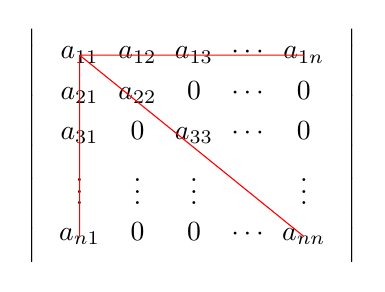
\begin{tikzpicture}
      \matrix(A) [matrix of math nodes,nodes in empty cells,ampersand replacement=\&,left delimiter=|,right delimiter=|] {
        a_{11} \& a_{12} \& a_{13} \& \cd \& a_{1n} \\
        a_{21} \& a_{22} \& 0     \& \cd \&  0    \\
        a_{31} \&  0    \& a_{33} \& \cd \&  0    \\
        \vd  \&  \vd  \&  \vd  \&     \&  \vd  \\
        a_{n1} \&  0    \& 0 \& \cd \& a_{nn} \\
      };
      \draw[red] (A-1-1.center) -- (A-1-5.center) (A-1-1.center) -- (A-5-1.center) (A-1-1.center) -- (A-5-5.center);
    \end{tikzpicture}
  \end{center}
  \pause 
  其解法固定,即从第二行开始,每行依次乘一个系数然后加到第一行,使得第一行除第一个元素外都为零,从而得到一个下三角行列式。

\end{frame}


\begin{frame}
  计算行列式(假定$a_i \ne 0$)
  $$
  D_{n+1} = 
  \left|
  \begin{array}{ccccc}
    a_0 &  1  & 1   &\cd & 1   \\
    1   & a_1 & 0   &\cd & 0  \\
    1   & 0   & a_2 &\cd & 0  \\
    \vd & \vd  \vd  &    & \\
    1   & 0   & 0   &\cd & a_n
  \end{array}
  \right| \pause = (a_0 - \sum_{i=1}^n \frac1{a_i}) a_1 a_2 \cd a_n.
  $$

  
\end{frame}


\begin{frame}
类似的方式还可用于求解如下形式的“爪型行列式”
  \begin{figure}
    \centering
    \subfigure[]{
      
\begin{tikzpicture}
        \matrix(B) [matrix of math nodes,nodes in empty cells,ampersand replacement=\&,left delimiter=|,right delimiter=|] {
          \&  \& \\
          \&  \& \\
          \&  \& \\ 
        };
        \draw[red] (B-1-3.north east) -- (B-1-1.north west) 
        (B-1-3.north east) -- (B-3-1.south west) 
        (B-1-3.north east) -- (B-3-3.south east);
      \end{tikzpicture}
    }
    \subfigure[]{
      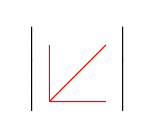
\begin{tikzpicture}
        \matrix(B) [matrix of math nodes,nodes in empty cells,ampersand replacement=\&,left delimiter=|,right delimiter=|] {
          \&  \& \\
          \&  \& \\
          \&  \& \\
        };
        \draw[red]
        (B-3-1.south west) -- (B-1-1.north west) 
        (B-3-1.south west) -- (B-1-3.north east) 
        (B-3-1.south west) -- (B-3-3.south east);
      \end{tikzpicture}
    }
    \subfigure[]{
      
\begin{tikzpicture}
        \matrix(B) [matrix of math nodes,nodes in empty cells,ampersand replacement=\&,left delimiter=|,right delimiter=|] {
          \&  \& \\
          \&  \& \\
          \&  \& \\
        };
        \draw[red]
        (B-3-3.south east) -- (B-1-1.north west) 
        (B-3-3.south east) -- (B-1-3.north east) 
        (B-3-3.south east) -- (B-3-1.south west);
      \end{tikzpicture}
    }
      
    \end{figure}
\end{frame}


\begin{frame}
  \begin{exampleblock}{例8}
    $$
    \left|
    \begin{array}{ccccc}
      1 & 1 & \cd & 1 & 1 \\
      0 & 0 & \cd & 2 & 1 \\
      \cd & \cd & & \cd & \cd \\
      0 & n-1 & \cd & 0 & 1 \\
      n & 0 & \cd & 0 & 1
    \end{array}
    \right| \pause = (-1)^{\frac{n(n-1)}2} n! \left(1-\sum_{i=2}^n\frac1i\right)
    $$
  \end{exampleblock}
\end{frame}

    
\begin{frame}
  \begin{exampleblock}{例9}
    计算$n$阶行列式
    $$
    D_n = \left|
    \begin{array}{cccc}
      x & a & \cd & a \\
      a & x & \cd & a \\
      \vd & \vd & & \vd \\
      a & a &  \cd & x 
    \end{array}
    \right|
    $$
  \end{exampleblock}
  
\end{frame}

    
\begin{frame}
  
  \begin{center}
    \red{方法一}
  \end{center}
  $$
  \begin{array}{rcl}
    D_n  
    & \pause \xlongequal{c_1+c_2+\cd +c_n}& \pause 
    \left|
    \begin{array}{cccc}
      x+(n-1)a & a     & \cd & a \\
      x+(n-1)a & x     & \cd & a \\
      \vd &      \vd &  & \vd \\
      x+(n-1)a & a     & \cd & x 
    \end{array}
    \right|  \\[1.0cm] 
    & \pause \xlongequal{c_1\div [x+(n-1)a] } & \pause 
             \left[x+(n-1)a\right]\left|
             \begin{array}{cccc}
               1 & a     & \cd & a \\
               1 & x     & \cd & a \\
               \vd   & \vd &  & \vd \\
              1 & a     & \cd & x 
            \end{array}
            \right|  \\[1.0cm]
            & \pause \xlongequal[i = 2, \cd, n]{r_i - r_1} & \pause
            \left[x+(n-1)a\right]\left|
            \begin{array}{cccc}
              1 & a   & \cd & 0 \\
              0 & x-a & \cd & 0 \\
              \vd  & \vd &  & \vd \\
              0 & 0   & \cd & x-a 
            \end{array}
            \right| \\[1.0cm]
            & \pause= & \pause \left[x+(n-1)a\right](x-a)^{n-1}
  \end{array}
  $$
\end{frame}
    
    

\begin{frame}
  \begin{center}
    \red{方法二}
  \end{center}

  $$
  \begin{array}{rcl}
    D_n 
    & \pause \xlongequal[i=2,\cd, n]{r_i - r_1} &  \pause
    \left|
    \begin{array}{ccccc}
      x   & a   & a    & \cd & a \\
      a-x & x-a & 0    & \cd & 0 \\
      a-x & 0   & x-a  & \cd & 0 \\
      \vd & \vd  & \vd &  & \vd \\
      a-x & 0   & 0    & \cd & x-a 
    \end{array}
    \right| \\[0.6in]
    & \pause \xlongequal[i=2,\cd,n]{c_1+c_i} & \pause
    \left|
    \begin{array}{ccccc}
      x+(n-1)a & a   & a    & \cd & a \\
      0    & x-a & 0    & \cd & 0 \\
      0    & 0   & x-a  & \cd & 0 \\
      \vd & \vd  & \vd &  & \vd \\
      0    & 0   & 0    & \cd & x-a 
    \end{array}
    \right|   \\[0.6in]
    & \pause = & \pause  \left[x+(n-1)a\right](x-a)^{n-1}.
  \end{array}
  $$
\end{frame}

\begin{frame}
  \begin{center}
    \red{方法三(升阶法)}
  \end{center}
  \begin{small}
      $$
  D_n = \left|
  \begin{array}{ccccc}
    \red{1}   & \red{a}  & \red{a}  & \red{\cd} & \red{a}   \\
    \red{0}   & x  & a  & \cd & a   \\
    \red{0}   & a  & x  & \cd & a   \\
    \red{\vd} &\vd &\vd &     & \vd \\
    \red{0}   & a  & a  & \cd & x 
  \end{array}
  \right|_{n+1} \pause 
  \xlongequal[i=2,\cdots,n+1]{r_i-r_1} \pause 
  \left|
  \begin{array}{ccccc}
    \red{1}    & \red{a}  & \red{a} & \red{\cd} & \red{a}   \\
    \red{-1}   & x-a      &  0      & \cd & 0   \\
    \red{-1}   & 0        &  x-a    & \cd & 0   \\
    \red{\vd}  &\vd       & \vd     &     & \vd \\
    \red{-1}   & 0        &   0     & \cd & x-a 
  \end{array}
  \right|_{n+1}
  $$
  \pause 
  \begin{itemize}
  \item
    若$x=a$,则$D_n=0$。 \pause \\
  \item 
    若$x\ne a$,则
    $$
    \begin{array}{rcl}
    D_n & \pause \xlongequal[j=2,\cd,n+1]{\disp c_1+ \frac1{x-a}c_j} & \pause 
    \left|
    \begin{array}{ccccc}
      \red{1+\frac{a}{x-a}n}   & \red{a}  & \red{a}  & \red{\cd} & \red{a}   \\
      \red{0}   & x-a  & 0  & \cd & 0   \\
      \red{0}   & 0  & x-a  & \cd & 0   \\
      \red{\vd} &\vd &\vd &     & \vd \\
      \red{0}   & 0  & 0  & \cd & x-a
    \end{array}
    \right|_{n+1} \\[0.5in]
    & \pause = & \pause  \left[x+(n-1)a\right](x-a)^{n-1}.
    \end{array}
    $$
  \end{itemize}

  \end{small}
\end{frame}

\begin{frame}
    \begin{center}
      \red{方法四}
    \end{center}

  \begin{footnotesize}    
    $$
    \begin{array}{ll}
      D_n & \pause = \left|
      \begin{array}{cccc}
        x-a  & a  & \cd & a   \\
        0    & x  & \cd & a   \\
        \vd  &\vd &     & \vd \\
        0    & a  & \cd & x 
      \end{array}
      \right|
      +\left|
      \begin{array}{cccc}
        a   & a  & \cd & a   \\
        a   & x  & \cd & a   \\
        \vd &\vd &     & \vd \\
        a   & a  & \cd & x 
      \end{array}
      \right| \\[1.0cm]
      &\pause = (x-a) D_{n-1} + a(x-a)^{n-1}.
    \end{array}
    $$ \pause 
    于是
    $$
    \left\{
    \begin{array}{rcl}
      D_n           &=& (x-a)D_{n-1} + a(x-a)^{n-1} \\[0.2cm]
      (x-a)D_{n-1}      &=& (x-a)^2D_{n-2} + a(x-a)^{n-1} \\[0.2cm]
      \cd           && \\ [0.2cm]
      (x-a)^{n-4}D_4 &=& (x-a)^{n-3}D_{3} + a(x-a)^{n-1}\\ [0.2cm]
      (x-a)^{n-3}D_3 &=& (x-a)^{n-2}D_{2} + a(x-a)^{n-1}
    \end{array}
    \right.
    $$ \pause 
    因此
    $$
    D_n = (x-a)^{n-2}(x^2-a^2) + (n-2)a(x-a)^{n-1} = [x+(n-1)a](x-a)^{n-1}      
    $$
  \end{footnotesize}
\end{frame}


\begin{frame}
    该行列式经常以不同方式出现,如
    \begin{itemize}
    \item
      $$
      \left|
      \begin{array}{cccc}
        0  &  1  & \cd & 1   \\
        1  &  0  & \cd & 1   \\
        \vd& \vd &     & \vd \\
        1  &  1  & \cd & 0 
      \end{array}
      \right| \pause  = (-1)^{n-1}(n-1)
      $$ \pause 
    \item
      $$
      \left|
      \begin{array}{cccc}
        1  &  a  & \cd & a   \\
        a  &  1  & \cd & a   \\
        \vd& \vd &     & \vd \\
        a  &  a  & \cd & 1
      \end{array}
      \right| \pause
      = [1+(n-1)a](1-a)^{n-1}
      $$ \pause
    \item
      $$
      \left|
      \begin{array}{cccc}
        1+\lambda  &  1  & \cd & 1   \\
        1  &  1+\lambda  & \cd & 1   \\
        \vd& \vd &     & \vd \\
        1  &  1  & \cd & 1+\lambda 
      \end{array}
      \right| \pause
      = (\lambda+n)\lambda^{n-1}
      $$
    \end{itemize}

  
\end{frame}


\begin{frame}
    升阶法适用于求形如
    $$
    \left|
    \begin{array}{cccc}
      x_1 &  a  & \cd & a   \\
      a   & x_2 & \cd & a   \\
      \vd & \vd &     & \vd \\
      a   &  a  & \cd & x_n
    \end{array}
    \right|
    $$
    或
    $$
    \left|
    \begin{array}{cccc}
      x_1 & a_1  & \cd & a_n   \\
      a_1 & x_2 & \cd  & a_n   \\
      \vd & \vd &     & \vd \\
      a_1 & a_2  & \cd & x_n
    \end{array}
    \right|
    $$      
    的行列式。
\end{frame}


\begin{frame}
  $$
  \begin{array}{l}
      \left|
    \begin{array}{cccc}
      x_1 &  a  & \cd & a   \\
      a   & x_2 & \cd & a   \\
      \vd & \vd &     & \vd \\
      a   &  a  & \cd & x_n
    \end{array}
    \right| = \disp  (1+\sum_{i=1}^n \frac{a}{x_i-a})\prod_{i=1}^n(x_i-a)
    \\[0.5in]
    \left|
    \begin{array}{cccc}
      x_1 & a_1  & \cd & a_n   \\
      a_1 & x_2 & \cd  & a_n   \\
      \vd & \vd &     & \vd \\
      a_1 & a_2  & \cd & x_n
    \end{array}
    \right| = \disp (1+\sum_{i=1}^n \frac{a_i}{x_i-a_i})\prod_{i=1}^n(x_i-a_i)
  
  \end{array}
  $$      
\end{frame}

\begin{frame}
  \begin{center}
    \red{常见形式}
  \end{center}
    
    $$
    \left|
    \begin{array}{cccc}
      1+a &  1  & \cd & 1   \\
      2   & 2+a & \cd & 2  \\
      \vd & \vd &     & \vd \\
      n   &  n  & \cd & n+a
    \end{array}
    \right| \pause = \left[a+ \frac{n(n+1)}2\right]a^{n-1}
    $$
    或
    $$
    \left|
    \begin{array}{cccc}
      a_1+b & a_1   & \cd & a_n   \\
      a_1   & a_2+b & \cd  & a_n   \\
      \vd   & \vd  &     & \vd \\
      a_1   & a_2   & \cd & a_n+b
    \end{array}
    \right| \pause = b^{n-1}(\sum_{i=1}^na_i+b)
    $$      
\end{frame}






\begin{frame}
  \begin{small}
    \begin{block}{例10}
      设
      $$
      \begin{array}{ll}
        D &= \left|
        \begin{array}{cccccc}
          a_{11} & \cd & a_{1k} &    &    &   \\
          \vd    &     &  \vd  &    &    &   \\
          a_{k1} & \cd & a_{kk} &    &    &   \\
          c_{11} & \cd & c_{1k} & b_{11}&  \cd & b_{1n}   \\
          \vd    &     & \vd   & \vd  &    & \vd \\
          c_{n1} & \cd & c_{nk} & b_{n1}&  \cd & b_{nn}
        \end{array}
        \right|, \\[1.0cm]
        D_1 &= det(a_{ij}) = \left|
        \begin{array}{ccc}
          a_{11} & \cd & a_{1k} \\
          \vd    &     &  \vd  \\
          a_{k1} & \cd & a_{kk} \\
        \end{array}
        \right|, \\[1.0cm]
        D_2 & = det(b_{ij}) = \left|
        \begin{array}{ccc}
          b_{11} & \cd & b_{1n} \\
          \vd    &     &  \vd  \\
          b_{n1} & \cd & b_{nn} \\
        \end{array}
        \right|.
      \end{array}
      $$
     证明:$D=D_1D_2$
    \end{block}
  \end{small}
\end{frame}

\begin{frame}
  \begin{footnotesize}
    \proofname
    对$D_1$做运算$r_i+\lambda r_j$将它转化成下三角行列式,设为
    $$
    D_1 =  \left|
    \begin{array}{ccc}
      p_{11} &       & \\
      \vd    & \dd  &  \\
      p_{k1} & \cd   & p_{kk} 
    \end{array}
    \right| = p_{11} \cd p_{kk}.
    $$\pause 
    对$D_2$做运算$c_i+\lambda c_j$将它转化成下三角行列式,设为
    $$
    D_2 =  \left|
    \begin{array}{ccc}
      q_{11} & \cd  &  q_{1n}\\
      & \dd  &  \vd \\
             &      & q_{nn} \\
    \end{array}
    \right| = q_{11}\cd q_{nn}.
    $$ \pause 
    于是,对$D$的前$k$行做运算$r_i+\lambda r_j$,对其后$n$列做运算$c_i+\lambda c_j$,把$D$转化为
    $$
    D = \left|
    \begin{array}{cccccc}
      p_{11} &      &  &    &    &   \\
      \vd    & \dd    &   &    &    &   \\
      p_{k1} & \cd & p_{kk} &    &    &   \\
      c_{11} & \cd & c_{1k} & q_{11}&  &    \\
      \vd    &     & \vd   & \vd  &  \dd  &  \\
      c_{n1} & \cd & c_{nk} & q_{n1}&  \cd & q_{nn}
    \end{array}
    \right|
    $$ \pause 
    故$D = p_{11}\cdots p_{kk} q_{11}\cdots q_{nn} = D_1 D_2$.
  \end{footnotesize}
\end{frame}



\begin{frame}
  \begin{footnotesize}
    \uncover<1->{
      \begin{exampleblock}{例11}
        计算$2n$阶行列式
        $$
        D_{2n} = \left|
        \begin{array}{cccccc}
          a &     & & & & b \\
          & \dd & & & \id & \\
          &   & a & b &  & \\
          &   & c & d &  &  \\
          & \id & & & \dd & \\
          c &     & & & & d
        \end{array}
        \right|
        $$
      \end{exampleblock}
    }
    \uncover<2->{
      \vspace{0.3cm}
      \textbf{解:} 把$D_{2n}$中的第$2n$行依次与第$2n-1$行、$\ldots$、第2行对调(共$2n-2$次相邻对换),
      在把第$2n$列依次与第$2n-1$列、$\ldots$、第2列对调,得
      $$
      D_{2n} = \left|
      \begin{array}{cccccccc}
        a & b & 0 &      & & & &0 \\
        c & d & 0 & & &  & &\\
        0 & 0 & a & & &  & & b \\
          &   &   & \dd &  &  & \id &   \\
          &   &   &     & a& b& & \\
        &   &   &     & c& d& & \\
        &   &   & \id &  &  & \dd &   \\
        0 & 0 & c & & &  & & d
      \end{array}
      \right|
      $$
    }
  \end{footnotesize}
\end{frame}

\begin{frame}
  \begin{footnotesize}
    故
    $$
    \begin{array}{ll}
      D_{2n} & = D_2 D_{2(n-1)}  \\[0.4cm]
      & = (ad-bc)D_{2(n-1)} \\[0.4cm]
      & = (ad-bc)^2 D_{2(n-2)}\\[0.4cm]
      & = \cdots \\[0.4cm]
      & = (ad-bc)^{n-1}D_{2} \\[0.4cm]
      & = (ad-bc)^n.      
    \end{array}
    $$
  \end{footnotesize}
\end{frame}


\begin{frame}
  \begin{footnotesize}
    \uncover<1->{
      \begin{exampleblock}{例12}
        证明范德蒙德(Vandermonde)行列式
        $$
        D_n = \left|
        \begin{array}{cccc}
          1        &  1        & \cd &    1     \\                    
          x_1      &  x_2      & \cd &    x_n    \\ 
          x_1^2    &  x_2^2     & \cd &   x_n^2   \\ 
          \vd      &  \vd      &     &    \vd      \\
          x_1^{n-1} & x_2^{n-1} &  \cd &  x_n^{n-1}
        \end{array}
        \right|
        = \prod_{n \ge i > j \ge 1}(x_i-x_j).
        $$
      \end{exampleblock}
    }
    \uncover<2->{
      \proofname
      用数学归纳法证明。当$n=2$时,
      $$
      D_2 = \left|
      \begin{array}{cc}
        1 & 1 \\
        x_1 & x_2
      \end{array}
      \right|
      = x_2 - x_1 = \prod_{2 \ge i > j \ge 1} (x_i - x_j),
      $$
      结论成立。
    }

  \end{footnotesize}
\end{frame}

\begin{frame}
  \begin{footnotesize}
    \proofname(续) \\[0.2cm]
    现假设结论对$n-1$阶范德蒙德行列式成立,以下证明结论对$n$阶范德蒙德行列式也成立。\pause 
    $$
    D_n \xlongequal[i=n,\cdots, 2]{\red{r_i - x_1 r_{i-1}}}\left|
    \begin{array}{ccccc}  
      1     & 1                    & 1                       & \cd   & 1    \\
      0     & x_2 - x_1            & x_3 - x_1               &  \cd  & x_n - x_1 \\
      0     & x_2(x_2 - x_1)       & x_3(x_3 - x_1)          &  \cd  & x_n(x_n - x_1)\\
      \vd   & \vd                  & \vd                     &      & \vd   \\
      0     & x_2^{n-2}(x_2-x_1)    & x_3^{n-2}(x_3 - x_1)    &  \cd  & x_n^{n-2}(x_n - x_1) 
    \end{array}\right|
    $$ \pause 
    按第1列展开,并把每列的公因子$(x_i-x_1)$提出,就有
    $$
    D_n = (x_2-x_1)(x_3-x_1)\cdots(x_n-x_1)\left|
    \begin{array}{cccc}  
      1            & 1          &  \cd  & 1 \\
      x_2          & x_3         &  \cd  & x_n\\
      \vd          & \vd         &      & \vd   \\
      x_2^{n-2}     & x_3^{n-2}    &  \cd  & x_n^{n-2}
    \end{array}\right|
    $$
    \pause 上式右端的行列式为$n-1$阶范德蒙德行列式,按归纳法假设,
    它等于所有$(x_i-x_j)$因子的乘积($n\ge i \ge j \ge 2$)。故
    $$
    D_n = (x_2-x_1)(x_3-x_1)\cdots(x_n-x_1) \prod_{n\ge i > j \ge 2}(x_i - x_j)
    = \prod_{n\ge i > j \ge 1}(x_i - x_j).
    $$
  \end{footnotesize}
\end{frame}

\begin{frame}
  \begin{footnotesize}
    \uncover<1->{
      \begin{exampleblock}{例13}
        设$a,b,c$为互不相同的实数,证明:
        $$
        \left|
        \begin{array}{ccc}
          1   &   1   &   1\\
          a   &   b   &   c\\
          a^3 &   b^3 &   c^3
        \end{array}
        \right|=0
        $$
        的充要条件是$a+b+c=0$.
      \end{exampleblock}
    }
    \uncover<2->{
      \vspace{0.3cm}
      \textbf{解:}考察范德蒙德行列式
      $$
      \begin{array}{ll}
        D & = \left|
        \begin{array}{cccc}
          1   &   1   &   1   & 1\\
          a   &   b   &   c   & y\\
          a^2 &   b^2 &   c^2 & y^2\\
          a^3 &   b^3 &   c^3 & y^3\\
        \end{array}
        \right|
        = (a-b)(a-c)(b-c)(a-y)(b-y)(c-y) 
      \end{array}
      $$
      
      注意到行列式$D$可看成是关于$y$的多项式,比较包含$y^2$的项:
      $$
      \cd - \left|
      \begin{array}{cccc}
        1   &   1   &   1  \\ 
        a   &   b   &   c  \\
        a^3 &   b^3 &   c^3\\
      \end{array}
      \right| y^2 + \cd = 
      \cd -(a-b)(a-c)(b-c)(a+b+c)y^2 + \cd 
      $$
    }      
  \end{footnotesize}
\end{frame}

\begin{frame}
  \begin{footnotesize}
    \textbf{解:}(续)
    于是
    $$
    (a-b)(a-c)(b-c)(a+b+c) = \left|
    \begin{array}{cccc}
      1   &   1   &   1  \\ 
      a   &   b   &   c  \\
      a^3 &   b^3 &   c^3\\
    \end{array}
    \right|
    = 0
    $$
    而$a,b,c$互不相同,故$a+b+c=0$.
  \end{footnotesize}
\end{frame}


\begin{frame}
  \begin{footnotesize}
  \begin{exampleblock}{例14}
    计算三对角行列式
    $$
    D_n = \left|
    \begin{array}{cccccc}
      a & b & &&&\\
      c&a&b&&&\\
      &c&a&b&&\\
      &&\dd&\dd&\dd&\\
      &&&c&a&b\\
      &&&&c&a
    \end{array}
    \right|
    $$
  \end{exampleblock}
    \textbf{解} 对$D_n$按第一行展开
    $$
    D_n = \pause aD_{n-1} + (-1)^{1+2} b \left|
    \begin{array}{cccccc}
      c&b&&&&\\
      0&a&b&&&\\
      0&c&a&b&&\\
      \vd&\vd&\dd&\dd&\dd&\\
      0&0&\cd&c&a&b\\
      0&0&\cd&0&c&a
    \end{array}
    \right| \pause = a D_{n-1} - bc D_{n-2}
    $$
    \pause 
    其中$$D_1=a, \quad D_2=a^2-bc$$.
  \end{footnotesize}
    
\end{frame}


\begin{frame}
  \begin{footnotesize}
    \textbf{解}
    将 
    $$D_n = a D_{n-1} - bc D_{n-2}$$
    改写成 \pause
    $$
    D_n - k D_{n-1} = l(D_{n-1} - k D_{n-2})
    $$ \pause
    这里
    $$
    k+l=a, \quad kl = bc.
    $$
    \pause
    令$\Delta_n = D_n-kD_{n-1}$,它满足
    $$
    \left\{
    \begin{array}{l}
      \Delta_n = l\Delta_{n-1},  \\[0.05in] \pause
      \Delta_2 = D_2-kD_1 = a^2-bc - ka = (a-k)a-kl=la-lk=l^2.
    \end{array}    
    \right.
    $$\pause 
    由此可知
    $$
    \Delta_n = l^{n-2} \Delta_2 = l^2, \pause
    $$
    即
    $$
    \begin{array}{rl}
    D_n & \pause = l^n  + k D_{n-1} \pause = l^n  + k (l^{n-1}  + k D_{n-2}) 
    \pause= l^n  + k l^{n-1}  + k^2 D_{n-2} \\[0.1in]
    & \pause=  l^n  + k l^{n-1}  + k^2 (l^{n-2}  + k D_{n-3} )
   \pause = l^n  + k l^{n-1}  + k^2 l^{n-2}  + k^3 D_{n-3} \\[0.1in]
    &\pause = \cd \pause =  l^n  + k l^{n-1}  + k^2 l^{n-2}  + \cd + k^{n-2}l^2 + k^{n-1} D_1
    \end{array}
    $$ \pause
    而$D_1 = a = k+l$,故
    $$
    \red{
    D_n = l^n  + k l^{n-1}  + k^2 l^{n-2}  + \cd + k^{n-2}l^2 + k^{n-1}l + k^n
    }
    $$
  \end{footnotesize}
\end{frame}

   %%%%%%%%%%%%
\section{克莱姆法则}

\begin{frame}
  \begin{footnotesize}
    考察$n$元一次方程组
    \begin{equation}\label{ls}
      \left\{
      \begin{array}{l}
        a_{11}x_1 + a_{12}x_2 + \cdots + a_{1n}x_n = b_1, \\[0.3cm]
        a_{21}x_1 + a_{22}x_2 + \cdots + a_{2n}x_n = b_2, \\[0.3cm]
        \cd \\[0.2cm]
        a_{n1}x_1 + a_{n2}x_2 + \cdots + a_{nn}x_n = b_n.
      \end{array}
      \right.
    \end{equation}
    与二、三元线性方程组相类似,它的解可以用$n$阶行列式表示。
  \end{footnotesize}
\end{frame}


\begin{frame}
  \begin{footnotesize}
    \begin{block}{克莱姆法则}
      如果线性方程组(\ref{ls})的系数行列式不等于0,即
      $$
      D = \left|
      \begin{array}{ccc}
        a_{11}  & \cd  & a_{1n} \\
        \vd    &      & \vd  \\
        a_{n1}  & \cd  & a_{nn}
      \end{array}
      \right|\ne 0
      $$
      则方程组(\ref{ls})存在唯一解
      $$
      x_1 = \frac{D_1}D, \ x_2 = \frac{D_2} D, \ \cdots, \ x_n = \frac{D_n}D,
      $$
      其中
      \begin{center}
        \begin{tikzpicture}
          \matrix (M) [matrix of math nodes]  { 
            D_j = \\
          };
          \matrix(MM) [right=2pt of M, matrix of math nodes,nodes in empty cells,
            ampersand replacement=\&,left delimiter=|,right delimiter=|] {
            a_{11} \& \cd \& a_{1,j-1} \&  b_1 \& a_{1, j+1} \& \cd \& a_{1n} \\
            \vd   \&     \& \& \vd \& \vd \& \vd \& \& \vd\\       
            a_{n1} \& \cd \&  a_{n,j-1} \&  b_n \& a_{n, j+1} \& \cd \& a_{nn} \\
          };
          \node[below=7pt  of MM-3-4, blue]  {第$j$列};
        \end{tikzpicture}
      \end{center}
    \end{block}
  \end{footnotesize}
\end{frame}

\begin{frame}
  \begin{footnotesize}
    \proofname
    \red{先证存在性}: 
    将$x_i=\frac{D_i}D$代入第$i$个方程,则有
    $$
    \begin{array}{cl}
      & a_{i1}x_1 +\cd + a_{ii}x_i + \cd + a_{in}x_n \\[0.3cm]
      & \pause=  \disp \frac1D(a_{i1}\red{D_1} +\cd + a_{ii}\blue{D_i} + \cd + a_{in}\purple{D_n}) \\[0.3cm]
      & \pause=  \disp \frac1D \left[
        a_{i1}\red{(b_1 A_{11}+ \cd + b_nA_{n1})}
        +\cd+ a_{ii}\blue{(b_1 A_{1i} + \cd + b_nA_{ni})}  \right. \\[0.2cm]
     & \pause \left. \ \ \ \ \ \
        + \cd + a_{in}\purple{(b_1 A_{1n}+ \cd + b_nA_{nn})} \right]\\[0.3cm]
     &\pause =  \disp \frac1D \left[
        b_1(a_{i1} A_{11}+ a_{i2} A_{12}  \cd + a_{in}A_{1n}) 
        +\cd + b_i(a_{i1} A_{i1}+ a_{i2} A_{i2}  \cd + a_{in}A_{in})   \right. \\[0.2cm]
        & \pause \left. \ \ \ \ \ \ + \cd+ b_n(a_{i1} A_{n1}+ a_{i2} A_{n2}  \cd + a_{in}A_{nn}) \right] \\[0.3cm]
      &\pause =  \disp \frac 1D b_{i} D = b_i.
    \end{array}
    $$
  \end{footnotesize}
\end{frame}

\begin{frame} 
  \begin{footnotesize}
    \proofname\textbf{[续]}\\
    \red{再证唯一性}:设还有一组解$\purple{y_i, i = 1, 2, \cd, n}$,以下证明$\purple{y_i =D_i/D}$。
    \pause 现构造一个新行列式
    $$
    \begin{array}{rcl}
      y_1D &\pause = &\pause \left|
      \begin{array}{cccc}
        a_{11}y_1 & a_{12}    &  \cd   &   a_{1n}      \\[0.1cm] 
        a_{21}y_1 & a_{22}    &  \cd   &   a_{2n}      \\[0.1cm] 
        \vd    &    \vd     &        &     \vd      \\[0.1cm] 
        a_{n1}y_1 & a_{n2}    &  \cd   &   a_{nn}      
      \end{array}
      \right| \\[0.4in]
      & \pause\xlongequal{c_1 + y_2 c_2 + \cd + y_n c_n} &\pause
      \left|
      \begin{array}{cccc}
        \sum_{k=1}^n a_{1k}y_k & a_{12}    &  \cd   &   a_{1n}      \\[0.1cm] 
        \sum_{k=1}^n a_{2k}y_k & a_{22}    &  \cd   &   a_{2n}      \\[0.1cm] 
        \vd    &    \vd     &        &     \vd      \\[0.1cm] 
        \sum_{k=1}^n a_{2k}y_k & a_{n2}    &  \cd   &   a_{nn}      
      \end{array}
      \right|  \\[0.4in]
      & \pause=&\pause \left|
      \begin{array}{cccc}
       b_1 & a_{12}    &  \cd   &   a_{1n}      \\[0.1cm] 
       b_2 & a_{22}    &  \cd   &   a_{2n}      \\[0.1cm] 
       \vd    &    \vd     &        &     \vd      \\[0.1cm] 
       b_n & a_{n2}    &  \cd   &   a_{nn}      
      \end{array}
      \right| \pause = D_1
    \end{array}
    $$\pause
    所以$y_1 = D_1/D$。\pause同理可证$y_i=D_i/D, i = 2, \cd, n$。
  \end{footnotesize}
\end{frame}


\begin{frame}
  \begin{footnotesize}
    \uncover<1->{
      \begin{exampleblock}{例}
        \setlength{\arraycolsep}{1.0pt}
        $$\left\{
        \begin{array}{rcrcrcrcr}
          2x_1 &+ & x_2 &- & 5x_3&+ & x_4 &= & 8, \\[0.2cm]
          x_1 &- & 3x_2&  &     &- & 6x_4& = & 9, \\[0.2cm]
          &  & x_2 &- & x_3 &+ & 2x_4 &= & -5, \\[0.2cm]
          x_1 &+ & 4x_2&-& 7x_3 &+& 6x_4 &= & 0.
        \end{array}
        \right.
        $$
      \end{exampleblock}
    }
    \uncover<2->{
      \vspace{0.3cm}
      \textbf{解:}
      $$
      \begin{array}{ll}
        D &= \left|
        \begin{array}{rrrr}
          2 &  1 & -5 &  1\\
          1 & -3 &  0 & -6\\
          0 &  2 & -1 &  2\\
          1 &  4 & -7 &  6
        \end{array}
        \right|
        \xlongequal[r_4-r_2]{r_1-2r_2}
        \left|
        \begin{array}{rrrr}
          0 &  7 & -5 & 13\\
          1 & -3 &  0 & -6\\
          0 &  2 & -1 &  2\\
          0 &  7 & -7 & 12
        \end{array}
        \right|\\[0.8cm]
        & = - \left|
        \begin{array}{rrr}
          7  & -5 & 13\\
          2  & -1 &  2\\
          7  & -7 & 12
        \end{array}
        \right|
        \xlongequal[c_3+2c_2]{c_1+2c_2}
        - \left|
        \begin{array}{rrr}
          -3  & -5 &  3\\
          0  & -1 &  0\\
          -7 & -7 & -2
        \end{array}
        \right|\\[0.8cm]
        & =\left| 
        \begin{array}{rr}
          -3 &  3\\
          -7 & -2
        \end{array}
        \right| = 27.
      \end{array}
      $$
    }
  \end{footnotesize}
\end{frame}


\begin{frame}
  \begin{footnotesize}
    \textbf{解:}(续)
    $$
    \begin{array}{ll}
      D_1 = \left|
      \begin{array}{rrrr}
        \red{8}  &  1 & -5 &  1\\
        \red{9}  & -3 &  0 & -6\\
        \red{-5} &  2 & -1 &  2\\
        \red{0}  &  4 & -7 &  6
      \end{array}
      \right|= 81, &
      D_2 = \left|
      \begin{array}{rrrr}
        2 & \red{8}  & -5 &  1\\
        1 & \red{9}  &  0 & -6\\
        0 & \red{-5} & -1 &  2\\
        1 & \red{0}  & -7 &  6
      \end{array}
      \right|=-108,\\[0.8cm]
      D_3 = \left|
      \begin{array}{rrrr}
        2  &  1 & \red{8}  &  1\\
        1  & -3 & \red{9}  & -6\\
        0  &  2 & \red{-5} &  2\\
        1  &  4 & \red{0}  &  6
      \end{array}
      \right|= -27, &
      D_4 = \left|
      \begin{array}{rrrr}
        2 &  1 & -5 & \red{8} \\
        1 & -3 &  0 & \red{9} \\
        0 &  2 & -1 & \red{-5}\\
        1 &  4 & -7 & \red{0} 
      \end{array}
      \right|= 27
    \end{array}
    $$
    于是得
    $$
    x_1 = \frac{D_1}D = 3,  \ \ 
    x_2 = \frac{D_2}D = -4, \ \ 
    x_3 = \frac{D_3}D = -1, \ \ 
    x_4 = \frac{D_4}D = 1.
    $$
  \end{footnotesize}
\end{frame}


\begin{frame}
  \begin{footnotesize}
    \uncover<1->{
      \begin{exampleblock}{例}
        设曲线$y=a_0+a_1x + a_2 x^2 + a_3 x^3$通过四点$(1,3), (2,4), (3,3), (4,-3)$,
        求系数$a_0,a_1,a_2,a_3$。
      \end{exampleblock}
    }
    \uncover<2->{
      \vspace{0.3cm}
      \textbf{解:}依题意可得线性方程组

      $$
      \setlength{\arraycolsep}{1.0pt}
      \left\{
      \begin{array}{rcrcrcrcr}
        a_0 & + &  a_1 & + &  a_2 & + &   a_3 & = & 3, \\[0.2cm]
        a_0 & + & 2a_1 & + & 4a_2 & + &  8a_3 & = & 4, \\[0.2cm]
        a_0 & + & 3a_1 & + & 9a_3 & + & 27a_3 & = & 3, \\[0.2cm]
        a_0 & + & 4a_1 & + &16a_4 & + & 64a_3 & = & 3,
      \end{array}
      \right.
      $$
      其系数行列式为
      $$
      D = \left|
      \begin{array}{rrrr}
        1 & 1 &  1 &  1 \\
        1 & 2 &  4 &  8 \\
        1 & 3 &  9 & 27 \\
        1 & 4 & 16 & 64
      \end{array}
      \right|
      $$
      是一个范德蒙德行列式,其值为
      $$ 
      D = 1\cdot 2 \cdot 3 \cdot 1 \cdot 2 \cdot 1 = 12
      $$
    }

  \end{footnotesize}
\end{frame}


\begin{frame}
  \begin{footnotesize}
    \textbf{解:}(续)
    $$
    \begin{array}{ll}
      D_1 = \left|
      \begin{array}{rrrr}
        \red{3}  &  1 &  1 &  1\\
        \red{4}  &  2 &  4 &  8\\
        \red{3}  &  3 &  9 & 27\\
        \red{-3} &  4 & 16 & 64
      \end{array}
      \right|= 36, &
      D_2 = \left|
      \begin{array}{rrrr}
        1 & \red{3}  & 1  &  1\\
        1 & \red{4}  & 4  &  8\\
        1 & \red{3}  & 8  &  27\\
        1 & \red{-3} & 16 &  64
      \end{array}
      \right|=-18,\\[0.8cm]
      D_3 = \left|
      \begin{array}{rrrr}
        1 & 1 & \red{3}  &  1 \\
        1 & 2 & \red{4}  &  8 \\
        1 & 3 & \red{3}  & 27 \\
        1 & 4 & \red{-3} & 64
      \end{array}
      \right|= 24, &
      D_4 = \left|
      \begin{array}{rrrr}
        1 & 1 &  1 & \red{3} \\
        1 & 2 &  4 & \red{4} \\
        1 & 3 &  9 & \red{3} \\
        1 & 4 & 16 & \red{-3}
      \end{array}
      \right|= -6.
    \end{array}
    $$
    于是得
    $$
    a_0 = \frac{D_1}D = 3,  \ \ 
    a_1 = \frac{D_2}D = -3/2, \ \ 
    a_2 = \frac{D_3}D = 2, \ \ 
    a_3 = \frac{D_4}D = -1/2.
    $$
    即曲线方程为
    $$
    y = 3 - \frac 32 x + 2 x^2 - \frac 12 x^3.
    $$
  \end{footnotesize}
  
\end{frame}


\begin{frame}
  \begin{footnotesize}
    \begin{block}{定理}
      如果线性方程组(\ref{ls})的系数行列式$D\ne 0$,则(\ref{ls})一定有解,且解是惟一的。
    \end{block}

    \begin{block}{定理}
      如果线性方程组(\ref{ls})无解或有两个不同的解,则它的系数行列式必为0。
    \end{block}

    \vspace{0.3cm}
    \textbf{说明:} \\
    \begin{itemize}
    \item 
      线性方程组(\ref{ls})右端的常数项$b_1,b_2,\cd, b_n$不全为0时,
      线性方程组(\ref{ls})叫做\red{非齐次线性方程组}\\[0.2cm]
      当$b_1,b_2,\cd, b_n$全为0时,
      线性方程组(\ref{ls})叫做\red{齐次线性方程组}。
    \end{itemize}

  \end{footnotesize}
\end{frame}


\begin{frame}
  \begin{footnotesize}
    \begin{block}{齐次线性方程组}
      对于齐次线性方程组
      \begin{equation}\label{ls0}
        \left\{
        \begin{array}{l}
          a_{11}x_1 + a_{12}x_2 + \cdots + a_{1n}x_n = 0, \\[0.3cm]
          a_{21}x_1 + a_{22}x_2 + \cdots + a_{2n}x_n = 0, \\[0.3cm]
          \cd \\[0.2cm]
          a_{n1}x_1 + a_{n2}x_2 + \cdots + a_{nn}x_n = 0.
        \end{array}
        \right.
      \end{equation}
      一定有零解,但不一定有非零解。
    \end{block}
  \end{footnotesize}
\end{frame}

\begin{frame}
  \begin{footnotesize}
    \begin{block}{定理}
      如果齐次线性方程组(\ref{ls0})的系数行列式$D\ne 0$,则它没有非零解。
    \end{block}

    \vspace{1.0cm}
    
    \begin{block}{定理}
      如果齐次线性方程组(\ref{ls0})有非零解,则它的系数行列式必为0。
    \end{block}
    
  \end{footnotesize}
\end{frame}


\begin{frame}
  \begin{footnotesize}
    \uncover<1->{
      当$\lambda$为何值时,齐次线性方程组
      $$
      \left\{
      \begin{array}{rcrcrcr}
        (5-\lambda) x & + &           2 y & + & 2           z & = & 0, \\
        2           x & + & (6-\lambda) y &   &               & = & 0, \\
        2           x &   &               & + & (4-\lambda) z & = & 0.
      \end{array}
      \right.
      $$
      有非零解?
    }

    \uncover<2->{
      \vspace{0.3cm}
      \textbf{解:}由上述定理可知,若所给齐次线性方程组有非零解,则其系数行列式$D=0$。
      而
      $$
      \begin{array}{ll}
        D & = \left|
        \begin{array}{ccc}
          5-\lambda & 2         & 2  \\
          2         & 6-\lambda & 0  \\
          2         & 0         & 4-\lambda
        \end{array}
        \right| \\[0.8cm]
        & = (5-\lambda)(6-\lambda)(4-\lambda) - 4(4-\lambda) - 4(6-\lambda)\\[0.3cm]
        & = (5-\lambda)(2-\lambda)(8-\lambda),
      \end{array}
      $$
      故$\lambda=2$、$\lambda=5$或$\lambda=8$。
    }

  \end{footnotesize}
\end{frame}

  \section{习题}

\begin{frame}
  \begin{footnotesize}
    \begin{exampleblock}{1}
      $$
      \left|
      \begin{array}{rr}
        a^2&ab\\
        ab&b^2
      \end{array}
      \right|
      $$
    \end{exampleblock}
    \pause 
    \jiename
    $$
    \mbox{原式} = a^2b^2-(ab)(ab) = 0.
    $$    
  \end{footnotesize}
\end{frame}


\begin{frame}
  \begin{footnotesize}
    \begin{exampleblock}{2}
      $$
      \left|
      \begin{array}{rr}
        \cos \alpha& -\sin \alpha\\
        \sin \alpha&  \cos \alpha
      \end{array}
      \right|
      $$
    \end{exampleblock}
    \pause 
    \jiename
    $$
    \mbox{原式} = \cos^2\alpha + \sin^2 \alpha= 1.
    $$    
  \end{footnotesize}
\end{frame}

\begin{frame}
  \begin{footnotesize}
    \begin{exampleblock}{3}
      $$
      \left|
      \begin{array}{cc}
        a+bi&b\\
        2a&a-bi
      \end{array}
      \right|
      $$      
    \end{exampleblock}
    \pause 
    \jiename
    $$
    \mbox{原式} = (a+bi)(a-bi)-2ab = a^2+b^2-2ab=(a-b)^2.
    $$ 
  \end{footnotesize}
\end{frame}


\begin{frame}
  \begin{footnotesize}
    \begin{exampleblock}{4}
      $$
      \left|
      \begin{array}{rrr}
        3&2&-4\\
        4&1&-2\\
        5&2&-3
      \end{array}
      \right|
      $$
    \end{exampleblock}
    \pause 
    \jiename
    \begin{center}
      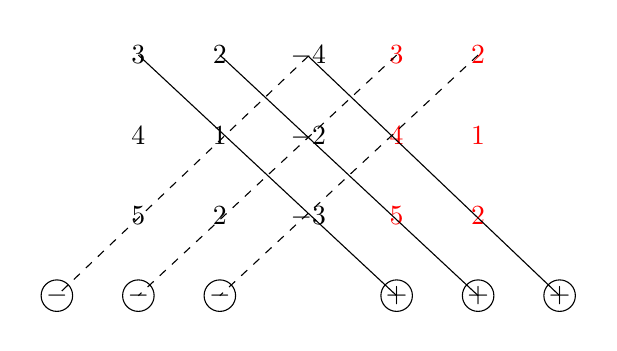
\begin{tikzpicture}               
        \matrix(A) [matrix of math nodes,nodes in empty cells,ampersand replacement=\&,row sep=15pt,column sep=15pt] {
          \&  3 \& 2 \& -4  \& \red{3} \& \red{2} \&\\
          \&  4 \& 1 \& -2  \& \red{4} \& \red{1} \&\\
          \&  5 \& 2 \& -3  \& \red{5} \& \red{2} \&\\
          -   \&    -        \&   -        \&               \&   +         \&   +        \& +\\
        };
        \draw[] (A-1-2.center) -- (A-4-5.center);
        \draw[] (A-1-3.center)  -- (A-4-6.center);
        \draw[] (A-1-4.center) -- (A-4-7.center); 
        \draw[dashed] (A-1-6.center) -- (A-4-3.center);
        \draw[dashed] (A-1-5.center) -- (A-4-2.center);
        \draw[dashed] (A-1-4.center) -- (A-4-1.center);
        \draw (A-4-1.center) circle (0.2cm);
        \draw (A-4-2.center) circle (0.2cm);
        \draw (A-4-3.center) circle (0.2cm);
        \draw (A-4-5.center) circle (0.2cm);
        \draw (A-4-6.center) circle (0.2cm);
        \draw (A-4-7.center) circle (0.2cm);

      \end{tikzpicture}               
    \end{center}
    \pause 
    $$
    \begin{array}{rl}
      \mbox{原式} &=
      3\cdot1\cdot(-3)+2\cdot(-2)\cdot5+(-4)\cdot4\cdot2-(-4)\cdot1\cdot5-3\cdot(-2)\cdot2-2\cdot4\cdot(-3)\\[0.2cm]
      &= -9-20-32+20+12+24 = -5.
    \end{array}
    $$    
  \end{footnotesize}
\end{frame}


\begin{frame}
  \begin{footnotesize}
    \begin{exampleblock}{5}
      $$
      \left|
      \begin{array}{rrr}
        1&2&3\\
        4&5&6\\
        7&8&9
      \end{array}
      \right|
      $$
    \end{exampleblock}
    \pause 
    \jiename
    $$
    \mbox{原式} \xlongequal[r_2-r_1]{r_3-r_2}  \left|
    \begin{array}{ccc}
      1&2&3\\
      3&3&3\\
      3&3&3
    \end{array}
    \right|=0.
    $$    
  \end{footnotesize}
\end{frame}


\begin{frame}
  \begin{footnotesize}
    \begin{exampleblock}{6}
      $$
      \left|
      \begin{array}{rrr}
        2&2&1\\
        4&1&-1\\
        202&199&101
      \end{array}
      \right|
      $$
    \end{exampleblock}
    \pause 
    \jiename
    $$
    \begin{array}{rl}
      \mbox{原式} & \xlongequal[]{c_1-c_2}  \left|
      \begin{array}{rrr}
        0&2&1\\
        3&1&-1\\
        3&199&101
      \end{array}
      \right| \xlongequal[]{r_3-r_2}  \left|
      \begin{array}{rrr}
        0&2&1\\
        3&1&-1\\
        0&198&102
      \end{array}
      \right| \\[0.2in]
      & = (-1)^{2+1}\cdot 3 \cdot \left|
      \begin{array}{rr}
        2&1\\
        198&102
      \end{array}
      \right| = -3 \cdot  (2\cdot 102-198)=-18.
    \end{array}
    $$    
  \end{footnotesize}
\end{frame}


\begin{frame}
  \begin{footnotesize}
    \begin{exampleblock}{7}
      $$
      \left|
      \begin{array}{ccc}
        1&\omega&\omega^2\\
        \omega^2&1&\omega\\
        \omega&\omega^2&1
      \end{array}
      \right|, \quad \omega = -\frac12 + i \frac{\sqrt{3}}2
      $$
    \end{exampleblock}
    \pause 
    \jiename 注意到$\omega^3=1$,故
    $$
    \omega \left|
    \begin{array}{ccc}
      1&\omega&\omega^2\\
      \omega^2&1&\omega\\
      \omega&\omega^2&1
    \end{array}
    \right| = \left|
    \begin{array}{ccc}
      1&\omega&\omega^2\\
      \omega^3&\omega&\omega^2\\
      \omega&\omega^2&1
    \end{array}
    \right| = \left|
    \begin{array}{ccc}
      1&\omega&\omega^2\\
      1&\omega&\omega^2\\
      \omega&\omega^2&1
    \end{array}
    \right| = 0,
    $$
    从而
    $$
    \mbox{原式}=0.
    $$
  \end{footnotesize}
\end{frame}


\begin{frame}
  \begin{footnotesize}
    \begin{exampleblock}{8}
      $$
      \left|
      \begin{array}{ccc}
        1&x&x\\
        x&2&x\\
        x&x&3
      \end{array}
      \right|.
      $$
    \end{exampleblock}
    \pause 
    \jiename 
    $$
    \begin{array}{rl}
      \mbox{原式} & \xlongequal[r_3-xr_1]{r_2-xr_1} \left|
      \begin{array}{ccc}
        1&x&x\\
        0&2-x^2&x-x^2\\
        0&x-x^2&3-x^2
      \end{array}
      \right| = \left|
      \begin{array}{cc}
        2-x^2&x-x^2\\
        x-x^2&3-x^2
      \end{array}
      \right| \\[0.2in]
      &= (2-x^2)(3-x^2)-(x-x^2)^2=2x^3-6x^2+6.      
    \end{array}
    $$
  \end{footnotesize}
\end{frame}

\begin{frame}
  \begin{footnotesize}
    \begin{exampleblock}{9}
      $$
      \left|
      \begin{array}{cccc}
        0&0&0&4\\
        0&0&4&3\\
        0&4&3&2\\
        4&3&2&1\\
      \end{array}
      \right|
      $$
    \end{exampleblock}
    \pause 
    \jiename 
    $$
    \begin{array}{rl}
      \mbox{原式} & = (-1)^{1+4} \cdot 4 \cdot \left|
      \begin{array}{cccc}
        0&0&\red{4}\\
        0&4&3\\
        4&3&2\\
      \end{array}
      \right| \\[0.2in]
      & = (-1)^{1+4} \cdot 4 \cdot (-1)^{1+3} \cdot 4 \cdot \left|
      \begin{array}{cccc}
        0&4\\
        4&3\\
      \end{array}
      \right| \\[0.2in]
      & = -4\cdot 4 \cdot (-16) = 256.
    \end{array}
    $$
  \end{footnotesize}
\end{frame}



\begin{frame}
  \begin{footnotesize}
    \begin{exampleblock}{10}
      $$
      \left|
      \begin{array}{cccccc}
        0&0&\cd&0&1&0\\
        0&0&\cd&2&0&0\\
        \vd&\vd&&\vd&\vd&\vd\\
        0&8&\cd&0&0&0\\
        9&0&\cd&0&0&0\\
        0&0&\cd&0&0&10\\
      \end{array}
      \right|
      $$
    \end{exampleblock}
    \pause 
    \jiename 
    $$
    \begin{array}{rl}
      \mbox{原式} & = (-1)^{10+10} \cdot 10 \cdot \left|
      \begin{array}{cccccc}
        0&0&\cd&0&1\\
        0&0&\cd&2&0\\
        \vd&\vd&&\vd&\vd\\
        0&8&\cd&0&0\\
        9&0&\cd&0&0\\
      \end{array}
      \right| = 10 \cdot (-1)^{\frac{9\times 8}2} 9! = 10!
    \end{array}
    $$
  \end{footnotesize}
\end{frame}


\begin{frame}
  \begin{footnotesize}
    \begin{exampleblock}{11}
      $$
      \left|
      \begin{array}{rrrr}
        1&1&1&1\\
        1&-1&1&1\\
        1&1&-1&1\\
        1&1&1&-1\\
      \end{array}
      \right|
      $$
    \end{exampleblock}
    \pause 
    \jiename 
    $$
    \mbox{原式}  \xlongequal[i=2,3,4]{r_i-r_1} \left|
    \begin{array}{rrrr}
      1&1&1&1\\
      0&-2&0&0\\
      0&0&-2&0\\
      0&0&0&-2
    \end{array}
    \right|  = (-2)^3 = -8.
    $$
  \end{footnotesize}
\end{frame}


\begin{frame}
  \begin{footnotesize}
    \begin{exampleblock}{12}
      $$
      \left|
      \begin{array}{rrrr}
        1&2&3&4\\
        2&3&4&1\\
        3&4&1&2\\
        4&1&2&3\\
      \end{array}
      \right|
      $$
    \end{exampleblock}
    \pause 
    \jiename 
    $$
    \begin{array}{rl}
      \mbox{原式}  & \xlongequal[i=4,3,2]{r_i-r_{i-1}} \left|
      \begin{array}{rrrr}
        1&2&3&4\\
        1&1&1&-3\\
        1&1&-3&1\\
        1&-3&1&1\\
      \end{array}
      \right| \pause
      \xlongequal[i=2,3,4]{c_i-c_1}  \left|
      \begin{array}{rrrr}
        1&1&2&3\\
        1&0&0&-4\\
        1&0&-4&0\\
        1&-4&0&0\\
      \end{array}
      \right| \\[0.25in] 
      & \pause \xlongequal[i=2,3,4]{c_i\div 4} 4^3 \left|
      \begin{array}{rrrr}
        1&\frac14&\frac24&\frac34\\
        1&0&0&-1\\
        1&0&-1&0\\
        1&-1&0&0\\
      \end{array}
      \right| \pause
      \xlongequal[]{c_1+c_2+c_3+c_4} 4^3 \left|
      \begin{array}{rrrr}
        1+\frac{1+2+3}4&\frac14&\frac24&\frac34\\
        0&0&0&-1\\
        0&0&-1&0\\
        0&-1&0&0\\
      \end{array}
      \right| \\[0.25in] 
      & \pause \ds =4^3 \frac{10}4 \left|
      \begin{array}{rrrr}
        0&0&-1\\
        0&-1&0\\
        -1&0&0\\
      \end{array}
      \right| = 160.
    \end{array}
    $$
  \end{footnotesize}
\end{frame}



\begin{frame}
  \begin{footnotesize}
    \begin{exampleblock}{13}
      $$
      \left|
      \begin{array}{rrrr}
        5&0&4&2\\
        1&-1&2&1\\
        4&1&2&0\\
        1&1&1&1\\
      \end{array}
      \right|
      $$
    \end{exampleblock}
    \pause 
    \jiename 
    $$
    \begin{array}{rl}
      \mbox{原式}  & \xlongequal[r_4+r_2]{r_3+r_2}
      \left|
      \begin{array}{rrrr}
        5&0&4&2\\
        1&\red{-1}&2&1\\
        5&0&4&1\\
        2&0&3&2\\
      \end{array}
      \right| \pause = (-1)^{2+2}\cdot (-1)\cdot       \left|
      \begin{array}{rrr}
        5&4&2\\
        5&4&1\\
        2&3&2\\
      \end{array}
      \right| \\[0.25in]
      & \pause \xlongequal[]{r_1-r_2}
      -\left|
      \begin{array}{rrr}
        0&0&\red{1}\\
        5&4&1\\
        2&3&2\\
      \end{array}
      \right| \pause
      = - (-1)^{1+3} \cdot 1 \cdot \left|
      \begin{array}{rrr}
        5&4\\
        2&3
      \end{array}
      \right| = -7.
    \end{array}
    $$
  \end{footnotesize}
\end{frame}

\begin{frame}
  \begin{footnotesize}
    \begin{exampleblock}{14}
      $$
      \left|
      \begin{array}{rrrrr}
        3&6&5&6&4\\
        2&5&4&5&3\\
        3&6&3&4&2\\
        2&5&4&6&5\\
        1&1&1&-1&-1
      \end{array}
      \right|
      $$
    \end{exampleblock}
    \pause 
    \jiename 
    $$
    \begin{array}{rl}
      \mbox{原式}  & \pause \xlongequal[]{r_2 \leftrightarrow r_3}
      -\left|
      \begin{array}{rrrrr}
        3&6&5&6&4\\
        3&6&3&4&2\\
        2&5&4&5&3\\
        2&5&4&6&5\\
        1&1&1&-1&-1
      \end{array}
      \right| \pause
      \xlongequal[r_1-r_3]{r_2-r_1 \atop r_4-r_3} -\left|
      \begin{array}{rrrrr}
        1&1&1&1&1\\
        0&0&-2&-2&-2\\
        2&5&4&5&3\\
        0&0&0&1&2\\
        1&1&1&-1&-1
      \end{array}
      \right| \\[0.4in]
      & \pause \xlongequal[r_5-r_1]{r_3-2r_1}  -\left|
      \begin{array}{rrrrr}
        1&1&1&1&1\\
        0&0&-2&-2&-2\\
        0&3&2&3&1\\
        0&0&0&1&2\\
        0&0&0&-2&-2
      \end{array}
      \right| \pause
      \xlongequal[r_5+2r_4]{r_2\leftrightarrow r_3}  \left|
      \begin{array}{rrrrr}
        1&1&1&1&1\\
        0&3&2&3&1\\
        0&0&-2&-2&-2\\
        0&0&0&1&2\\
        0&0&0&0&2
      \end{array}
      \right|\\[0.4in]
      & \pause = -12.
    \end{array}
    $$
  \end{footnotesize}
\end{frame}



\begin{frame}
  \begin{footnotesize}
    \begin{exampleblock}{15}
      $$
      \left|
      \begin{array}{rrrr}
        1&2&0&0\\
        3&4&0&0\\
        0&0&-1&3\\
        0&0&5&1\\
      \end{array}
      \right|
      $$
    \end{exampleblock}
    \pause 
    \jiename 
    $$
    \mbox{原式} = \left|
    \begin{array}{cc}
      1&2\\
      3&4      
    \end{array}
    \right| \cdot
    \left|
    \begin{array}{rr}
      -1&3\\
      5&1      
    \end{array}
    \right| = (-2)\cdot(-16)=32.
    $$
  \end{footnotesize}
\end{frame}


\begin{frame}
  \begin{footnotesize}
    \begin{exampleblock}{16}
      $$
      \left|
      \begin{array}{rrrrr}
        1&2&3&4&5\\
        6&7&8&9&10\\
        0&0&0&1&3\\
        0&0&0&2&4\\
        0&1&0&1&1
      \end{array}
      \right|
      $$
    \end{exampleblock}
    \pause 
    \jiename 
    $$
    \begin{array}{rl}
      \mbox{原式} & \pause \ds \xlongequal[]{r_3\leftrightarrow r_5}
      -\left|
      \begin{array}{rrrrr}
        \red{1}&\red{2}&\red{3}&4&5\\
        \red{6}&\red{7}&\red{8}&9&10\\
        \red{0}&\red{1}&\red{0}&1&1\\
        0&0&0&\blue{2}&\blue{4}\\
        0&0&0&\blue{1}&\blue{3}
      \end{array}
      \right| \pause = -\left|
      \begin{array}{rrr}
        1&2&3\\
        6&7&8\\
        0&\red{1}&0\\
      \end{array}
      \right| \cdot \left|
      \begin{array}{rr}
        2&4\\
        1&3\\
      \end{array}
      \right|\\[0.4in]
      &\pause =-(-1)^{3+2} \cdot 1 \cdot \left|
      \begin{array}{rrr}
        1&3\\
        6&8
      \end{array}
      \right| \cdot \left|
      \begin{array}{rr}
        2&4\\
        1&3\\
      \end{array}
      \right| \\[0.2in]
      &\pause =   (-10) \cdot 2 = -20.
    \end{array}
    $$
  \end{footnotesize}
\end{frame}

\begin{frame}
  \begin{footnotesize}
    \begin{exampleblock}{17}
      $$
      \left|
       \begin{array}{rrrrr}
        0&0&1&-1&2\\
        0&0&3&0&2\\
        0&0&2&4&0\\
        1&2&4&0&-1\\
        3&1&2&5&8
      \end{array}
      \right|
      $$
    \end{exampleblock}
    \pause 
    \jiename 
    $$
    \begin{array}{rl}
      \mbox{原式} &\pause
      \xlongequal[c_2\leftrightarrow c_1]{c_3\leftrightarrow c_2}
      \left|
      \begin{array}{rrrrr}
        1&0&0&-1&2\\
        3&0&0&0&2\\
        2&0&0&4&0\\
        4&1&2&0&-1\\
        2&3&1&5&8
      \end{array}
      \right|
      \pause
      \xlongequal[c_3\leftrightarrow c_2]{c_4\leftrightarrow c_3}
      \left|
      \begin{array}{rrrrr}
        1&-1&0&0&2\\
        3&0&0&0&2\\
        2&4&0&0&0\\
        4&0&1&2&-1\\
        2&5&3&1&8
      \end{array}
      \right| \\[0.35in]
      & \pause \xlongequal[c_4\leftrightarrow c_3]{c_5\leftrightarrow c_4}
      \left|
      \begin{array}{rrrrr}
        1&-1& 2&0&0\\
        3& 0& 2&0&0\\
        2& 4& 0&0&0\\
        4& 0&-1&1&2\\
        2& 5& 8&3&1
      \end{array}
      \right| \pause = \left|
      \begin{array}{rrrrr}
        1&-1& 2\\
        3& 0& 2\\
        2& 4& 0
      \end{array}
      \right|\cdot \left|
      \begin{array}{rr}
        1&2\\
        3&1
      \end{array}
      \right| \\[0.35in]
      & \pause \xlongequal[]{r_2-r_1} \left|
      \begin{array}{rrrrr}
        1&-1& 2\\
        2& 1& 0\\
        2& 4& 0
      \end{array}
      \right| \left|
      \begin{array}{rr}
        1&2\\
        3&1
      \end{array}
      \right| =   2  \left|
      \begin{array}{rrrrr}
        2& 1\\
        2& 4
      \end{array}
      \right| \left|
      \begin{array}{rr}
        1&2\\
        3&1
      \end{array}
      \right|  = 2 \cdot 6 \cdot (-5) = -60.
    \end{array}
    $$
  \end{footnotesize}
\end{frame}


\begin{frame}
  \begin{footnotesize}
    \begin{exampleblock}{18}
      $$
      \left|
      \begin{array}{cc}
        *&\A\\
        \B&\zero
      \end{array}
      \right|, \quad
      \A = \left|
      \begin{array}{ccc}
        1&0&0\\
        1&2&0\\
        1&2&3
      \end{array}
      \right|, \quad
      \B = \left|
      \begin{array}{rrrrr}
        &&&&-1\\
        &&&-2&\\
        &&-3&&\\
        &-4&&&\\
        -5&&&&
      \end{array}
      \right|
      $$
    \end{exampleblock}
    \pause
    \jiename   
    $$
    \begin{array}{rl}
      \mbox{原式} &\pause= (-1)^{3\times 5}  \left|
      \begin{array}{rr}
        \A&*\\
        \zero&\B
      \end{array}
      \right| \\[0.2in]
      &\pause = (-1) \cdot  |\A|\cdot |\B| \\[0.1in]
      &\pause= (-1) \cdot 1\cdot 2\cdot 3 \cdot (-1)^{\frac{5\times 4}2} (-1)(-2)(-3)(-4)(-5)\\[0.1in]
      &\pause= 6\times 120 =720
    \end{array}
    $$
  \end{footnotesize}
\end{frame}

\begin{frame}
  \begin{footnotesize}
    \begin{exampleblock}{19}
      证明:
      $$
      \left|
      \begin{array}{ccc}
        a_1+b_1x & a_1x+b_1 & c_1\\
        a_2+b_2x & a_2x+b_2 & c_2\\
        a_3+b_3x & a_3x+b_3 & c_3        
      \end{array}
      \right| = (1-x^2) \left|
      \begin{array}{ccc}
        a_1&b_1&c_1\\
        a_2&b_2&c_2\\
        a_3&b_3&c_3
      \end{array}
      \right|
      $$
    \end{exampleblock}
    \pause
    \proofname
    $$
    \begin{array}{rl}
      \mbox{左边} &\pause= \left|
      \begin{array}{ccc}
        a_1 & a_1x+b_1 & c_1\\
        a_2 & a_2x+b_2 & c_2\\
        a_3 & a_3x+b_3 & c_3        
      \end{array}
      \right| + \left|
      \begin{array}{ccc}
        b_1x & a_1x+b_1 & c_1\\
        b_2x & a_2x+b_2 & c_2\\
        b_3x & a_3x+b_3 & c_3        
      \end{array}
      \right|\\[0.2in]
      &\pause= \left|
      \begin{array}{ccc}
        a_1 & a_1x+b_1 & c_1\\
        a_2 & a_2x+b_2 & c_2\\
        a_3 & a_3x+b_3 & c_3        
      \end{array}
      \right| + x\left|
      \begin{array}{ccc}
        b_1 & a_1x+b_1 & c_1\\
        b_2 & a_2x+b_2 & c_2\\
        b_3 & a_3x+b_3 & c_3        
      \end{array}
      \right|\\[0.2in]
      &\pause= \left|
      \begin{array}{ccc}
        a_1 & a_1x & c_1\\
        a_2 & a_2x & c_2\\
        a_3 & a_3x & c_3        
      \end{array}
      \right| + \left|
      \begin{array}{ccc}
        a_1 & b_1 & c_1\\
        a_2 & b_2 & c_2\\
        a_3 & b_3 & c_3        
      \end{array}
      \right| +  x\left|
      \begin{array}{ccc}
        b_1 & a_1x & c_1\\
        b_2 & a_2x & c_2\\
        b_3 & a_3x & c_3        
      \end{array}
      \right| +  x\left|
      \begin{array}{ccc}
        b_1 & b_1 & c_1\\
        b_2 & b_2 & c_2\\
        b_3 & b_3 & c_3        
      \end{array}
      \right|\\[0.2in]
      &\pause=  \left|
      \begin{array}{ccc}
        a_1 & b_1 & c_1\\
        a_2 & b_2 & c_2\\
        a_3 & b_3 & c_3        
      \end{array}
      \right| +  x\left|
      \begin{array}{ccc}
        b_1 & a_1x & c_1\\
        b_2 & a_2x & c_2\\
        b_3 & a_3x & c_3        
      \end{array}
      \right| \pause = (1-x^2)\left|
      \begin{array}{ccc}
        a_1 & b_1 & c_1\\
        a_2 & b_2 & c_2\\
        a_3 & b_3 & c_3        
      \end{array}
      \right| = \mbox{右边}
    \end{array}
    $$
  \end{footnotesize}
\end{frame}

\begin{frame}
  \begin{footnotesize}
    \begin{exampleblock}{20}
      证明:
      $$
      \left|
      \begin{array}{cccc}
        1+x&1&1&1\\
        1&1-x&1&1\\
        1&1&1+y&1\\
        1&1&1&1-y
      \end{array}
      \right|=x^2y^2.
      $$
    \end{exampleblock}
    \pause
    \proofname
    $$
    \begin{array}{rl}
      \mbox{左边} & \pause = \left|
      \begin{array}{ccccc}
        \red{1}&\red{1}&\red{1}&\red{1}&\red{1}\\
        \red{0}&1+x&1&1&1\\
        \red{0}&1&1-x&1&1\\
        \red{0}&1&1&1+y&1\\
        \red{0}&1&1&1&1-y
      \end{array}
      \right| \\[0.4in]
      &\pause \xlongequal[i=2,3,4,5]{r_i-r_1} \left|
      \begin{array}{ccccc}
        \red{1}&\red{1}&\red{1}&\red{1}&\red{1}\\
        \red{-1}&x&0&0&0\\
        \red{-1}&0&-x&0&0\\
        \red{-1}&0&0&y&0\\
        \red{-1}&0&0&0&-y
      \end{array}
      \right|
      \pause
      \xlongequal[c_1+ c_4/y \atop c_1 -c_5/y ]{c_1+ c_2/x \atop c_1 -c_3/x } \left|
      \begin{array}{ccccc}
        \red{1}&\red{1}&\red{1}&\red{1}&\red{1}\\
        \red{0}&x&0&0&0\\
        \red{0}&0&-x&0&0\\
        \red{0}&0&0&y&0\\
        \red{0}&0&0&0&-y
      \end{array}
      \right| \\[0.4in]
      &\pause = x^2y^2.
    \end{array}
    $$
  \end{footnotesize}
\end{frame}

\begin{frame}
  \begin{footnotesize}
    \begin{exampleblock}{21}
      证明:
      $$
      \left|
      \begin{array}{ccc}
        1   &   1   &   1\\
        a   &   b   &   c\\
        a^3 &   b^3 &   c^3
      \end{array}
      \right| = (a-b)(a-c)(b-c)(a+b+c).
      $$
    \end{exampleblock}
    \pause
    \proofname
    考察范德蒙德行列式
    $$
    \left|
    \begin{array}{cccc}
      1   &   1   &   1   & \red{1}\\
      a   &   b   &   c   & \red{y}\\
      \red{a^2} &   \red{b^2} &   \red{c^2} & \purple{y^2}\\
      a^3 &   b^3 &   c^3 & \red{y^3}\\
    \end{array}
    \right|
    = (y-a)(y-b)(y-c)(c-a)(c-b)(b-a)
    $$
    \pause
    等式两端均为关于$y$的多项式,比较$y^2$的系数,可知
    $$
    \left|
    \begin{array}{cccc}
      1   &   1   &   1  \\ 
      a   &   b   &   c  \\
      a^3 &   b^3 &   c^3\\
    \end{array}
    \right| = (a-b)(a-c)(b-c)(a+b+c)
    $$

  \end{footnotesize}
\end{frame}

\begin{frame}
  \begin{footnotesize}
    \begin{exampleblock}{22}
      证明:
      $$
      \left|
      \begin{array}{ccc}
        1&a^2&a^3\\
        1&b^2&b^3\\
        1&c^2&c^3
      \end{array}
      \right| = (ab+bc+ca)\left|
      \begin{array}{ccc}
        1&a&a^2\\
        1&b&b^2\\
        1&c&c^2
      \end{array}
      \right|
      $$
    \end{exampleblock}
    \pause
    \proofname
    考察范德蒙德行列式
    $$
    \left|
    \begin{array}{cccc}      
      1&\red{a}&a^2&a^3\\
      1&\red{b}&b^2&b^3\\
      1&\red{c}&c^2&c^3\\
      \red{1}&\purple{y}&\red{y^2}&\red{y^3}
    \end{array}
    \right|
    = (y-a)(y-b)(y-c)(c-a)(c-b)(b-a)
    $$
    \pause
    等式两端均为关于$y$的多项式,比较$y$的系数,可知
    $$
    \left|
    \begin{array}{cccc}
      1   &   1   &   1  \\ 
      a^2 &   b^2 &   c^2  \\
      a^3 &   b^3 &   c^3\\
    \end{array}
    \right| = (a-b)(a-c)(b-c)(ab+bc+ca) = (ab+bc+ca)\left|
    \begin{array}{ccc}
      1&a&a^2\\
      1&b&b^2\\
      1&c&c^2
    \end{array}
    \right|
    $$

  \end{footnotesize}
\end{frame}


\begin{frame}
  \begin{footnotesize}
    \begin{exampleblock}{23}
      计算
      $$
      \left|
      \begin{array}{cccc}
        1&0&2&a\\
        2&0&b&0\\
        3&c&4&5\\
        d&0&0&0
      \end{array}
      \right|
      $$
    \end{exampleblock}
    \pause
    \jiename
    $$
    \begin{array}{rl}
      \mbox{左边} & \pause \xlongequal[]{\mbox{按第4行展开}}
      (-1)^{4+1} \cdot d \cdot \left|
      \begin{array}{ccc}
        0&2&a\\
        0&b&0\\
        c&4&5
      \end{array}
      \right| \\[0.4in]
      & \pause \xlongequal[]{\mbox{按第2行展开}}
      (-d) \cdot (-1)^{2+2} \cdot b \left|
      \begin{array}{ccc}
        0&a\\
        c&5
      \end{array}
      \right| = abcd.
    \end{array}
    $$
  \end{footnotesize}
\end{frame}


\begin{frame}
  \begin{footnotesize}
    \begin{exampleblock}{24}
      计算
      $$
      \left|
      \begin{array}{ccccc}
        a&1&0&0\\
       -1&b&1&0\\
        0&-1&c&1\\
        0&0&-1&d
      \end{array}
      \right|
      $$
    \end{exampleblock}
    \pause
    \jiename
    $$
    \begin{array}{rl}
      \mbox{左边} & \pause \xlongequal[]{\mbox{按第1行展开}}
      (-1)^{1+1} \cdot a \cdot \left|
      \begin{array}{ccc}        
        b&1&0\\
        -1&c&1\\
        0&-1&d
      \end{array}
      \right| + (-1)^{1+2} \cdot 1 \cdot\left|
      \begin{array}{ccccc}
        -1&1&0\\
        0&c&1\\
        0&-1&d
      \end{array}
      \right|
      \\[0.4in]
      & \pause = a \cdot \left|
      \begin{array}{ccc}        
        b&1&0\\
        -1&c&1\\
        0&-1&d
      \end{array}
      \right| +\left|
      \begin{array}{ccccc}
        c&1\\
        -1&d
      \end{array}
      \right|\\[0.4in]
      & \pause \xlongequal[]{\mbox{按第1行展开}}
      a \cdot \left( b \cdot \left|
      \begin{array}{ccc}
        c&1\\
        -1&d
      \end{array}
      \right| + (-1)^{1+2}\cdot 1 \cdot \left|
      \begin{array}{cc}
        -1&1\\
        0& d
      \end{array}
      \right| \right) + (cd+1)\\[0.2in]
      & \pause= a(b(cd+1)+d)+(cd+1) = (ab+1)(cd+1)+ad
    \end{array}
    $$
  \end{footnotesize}
\end{frame}

\begin{frame}
  \begin{footnotesize}
    \begin{exampleblock}{25}
      计算
      $$
      \left|
      \begin{array}{cccc}
        a^2&(a+1)^2&(a+2)^2&(a+3)^2\\[0.1cm]
        b^2&(b+1)^2&(b+2)^2&(b+3)^2\\[0.1cm]
        c^2&(c+1)^2&(c+2)^2&(c+3)^2\\[0.1cm]
        d^2&(d+1)^2&(d+2)^2&(d+3)^2
      \end{array}
      \right|
      $$
    \end{exampleblock}
    \pause
    \jiename
    $$
    \begin{array}{rl}
      \mbox{左边} & \pause \xlongequal[c_2-c_1]{c_4-c_3\atop c_3-c_2}
      \left|
      \begin{array}{cccc}
        a^2&2a+1&2a+3&2a+5\\[0.1cm]
        b^2&2b+1&2b+3&2b+5\\[0.1cm]
        c^2&2c+1&2c+3&2c+5\\[0.1cm]
        d^2&2d+1&2d+3&2d+5
      \end{array}
      \right|\\[0.4in]
      &\pause \xlongequal[c_3-c_2]{c_4-c_3}
      \left|
      \begin{array}{cccc}
        a^2&2a+1&2&2\\[0.1cm]
        b^2&2b+1&2&2\\[0.1cm]
        c^2&2c+1&2&2\\[0.1cm]
        d^2&2d+1&2&2
      \end{array}
      \right| = 0.
    \end{array}
    $$
  \end{footnotesize}
\end{frame}

\begin{frame}
  \begin{footnotesize}
    \begin{exampleblock}{26}
      计算
      $$
      \left|
      \begin{array}{cccc}
        a&b&c&1\\
        b&c&a&1\\
        c&a&b&1\\
        \frac{b+c}2&\frac{c+a}2&\frac{a+b}2&1        
      \end{array}
      \right|
      $$
    \end{exampleblock}
    \pause
    \jiename
    $$
    \mbox{原式} \pause \xlongequal[]{r_3+r_1+r_2}
    \left|
    \begin{array}{cccc}
      a&b&a+b+c&1\\
      b&c&a+b+c&1\\
      c&a&a+b+c&1\\
      \frac{b+c}2&\frac{c+a}2&a+b+c&1
    \end{array}
    \right| = 0 .
    $$
  \end{footnotesize}
\end{frame}


\begin{frame}
  \begin{footnotesize}
    \begin{exampleblock}{27}
      计算
      $$
      \left|
      \begin{array}{cccc}
        a_1&0&0&b_1\\
        0&a_2&b_2&0\\
        0&b_3&a_3&0\\
        b_4&0&0&a_4
      \end{array}
      \right|
      $$
    \end{exampleblock}
    \pause
    \jiename
    $$
    \begin{array}{rl}
      \mbox{原式} &\pause\xlongequal[c_3\leftrightarrow c_2]{c_4\leftrightarrow c_3}
      \left|
      \begin{array}{cccc}
        a_1&b_1&0  &  0\\
        0  &0  &a_2&b_2\\
        0  &0  &b_3&a_3\\
        b_4&a_4&0  &  0
      \end{array}
      \right|\\[0.4in]
      &\pause \xlongequal[r_3\leftrightarrow r_2]{r_4\leftrightarrow r_3}
      \left|
      \begin{array}{cccc}
        a_1&b_1&0  &  0\\
        b_4&a_4&0  &  0\\
        0  &0  &a_2&b_2\\
        0  &0  &b_3&a_3      
      \end{array}
      \right|
      \pause  = (a_1a_4-b_1b_4)(a_2a_3-b_2b_3) .
      
    \end{array}
    $$
  \end{footnotesize}
\end{frame}


\begin{frame}
  \begin{footnotesize}
    \begin{exampleblock}{28}
      计算
      $$
      \left|
      \begin{array}{cccccc}
        1&2&2&\cd&2&2\\
        2&2&2&\cd&2&2\\
        2&2&3&\cd&2&2\\
        \vd&\vd&\vd&\dd&\vd&\vd\\
        2&2&2&\cd&n-1&2\\
        2&2&2&\cd&2&n        
      \end{array}
      \right|
      $$
    \end{exampleblock}
    \pause
    \jiename
    $$
    \begin{array}{rl}
      \mbox{原式} &\pause = \left|
      \begin{array}{ccccccc}
        1&2&2&2&\cd&2&2\\
        0&1&2&2&\cd&2&2\\
        0&2&2&2&\cd&2&2\\
        0&2&2&3&\cd&2&2\\
        \vd&\vd&\vd&\vd&\dd&\vd&\vd\\
        0&2&2&2&\cd&n-1&2\\
        0&2&2&2&\cd&2&n        
      \end{array}
      \right| \pause = \left|
      \begin{array}{ccccccc}
        1&2&2&2&\cd&2&2\\
        -1&-1&0&0&\cd&0&0\\
        -1&0&0&0&\cd&0&0\\
        -1&0&0&1&\cd&0&0\\
        \vd&\vd&\vd&\vd&\dd&\vd&\vd\\
        -1&0&0&0&\cd&n-3&0\\
        -1&0&0&0&\cd&0&n-2        
      \end{array}
      \right|
    \end{array}
    $$
  \end{footnotesize}
\end{frame}

\begin{frame}
  \begin{footnotesize}
    $$
    \begin{array}{rl}
      \mbox{原式} &= \left|
      \begin{array}{ccccccc}
        1&2&2&2&\cd&2&2\\
        -1&-1&0&0&\cd&0&0\\
        \red{-1}&0&0&0&\cd&0&0\\
        -1&0&0&1&\cd&0&0\\
        \vd&\vd&\vd&\vd&\dd&\vd&\vd\\
        -1&0&0&0&\cd&n-3&0\\
        -1&0&0&0&\cd&0&n-2        
      \end{array}
      \right| \\[0.6in]
      &\pause =(-1)^{3+1} (-1)\left|
      \begin{array}{ccccccc}
        2&2&2&\cd&2&2\\
        -1&0&0&\cd&0&0\\
        0&0&1&\cd&0&0\\
        \vd&\vd&\vd&\dd&\vd&\vd\\
        0&0&0&\cd&n-3&0\\
        0&0&0&\cd&0&n-2        
      \end{array}
      \right|
      \\[0.2in]
      &\pause = -2 (n-2)!
    \end{array}
    $$    
  \end{footnotesize}
\end{frame}


\begin{frame}
  \begin{footnotesize}
    \begin{exampleblock}{29}
      计算
      $$
      \left|
      \begin{array}{ccccc}
        1&1&1&\cd&1\\[0.1cm]
        a&a-1&a-2&\cd&a-n\\[0.1cm]
        a^2&(a-1)^2&(a-2)^2&\cd&(a-n)^2\\[0.1cm]
        \vd&\vd&\vd&&\vd\\[0.1cm]
        a^n&(a-1)^n&(a-2)^n&\cd&(a-n)^n      
      \end{array}
      \right|
      $$      
    \end{exampleblock}
    \pause
    \jiename
    该行列式为范德蒙行列式,\pause 故
    $$
    \begin{array}{rl}
      \mbox{原式} & = \prod_{n\ge i > j \ge 0} [(a-i)-(a-j)] \\[0.4cm]
      &= \prod_{n\ge i > j \ge 0} (j-i) \\[0.4cm]
      & = (-1)^{\frac{n(n+1)}2} \prod_{n\ge i > j \ge 0} (i-j) \\[0.4cm]
      & = (-1)^{\frac{n(n+1)}2} \prod_{i=1}^n i!      
    \end{array}
    $$
  \end{footnotesize}
\end{frame}


\begin{frame}
  \begin{footnotesize}
    \begin{exampleblock}{30}
      计算
      $$
      \left|
      \begin{array}{cccccc}
        a_1^n&a_1^{n-1}b_1&a_1^{n-2}b_1^2&\cd&a_1b_1^{n-1}&b_1^n\\[0.1cm]
        a_2^n&a_2^{n-1}b_2&a_2^{n-2}b_2^2&\cd&a_2b_2^{n-1}&b_2^n\\[0.1cm]
        \vd&\vd&\vd&&\vd&\vd\\[0.1cm]
        a_{n+1}^n&a_{n+1}^{n-1}b_{n+1}&a_{n+1}^{n-2}b_{n+1}^2&\cd&a_{n+1}b_{n+1}^{n-1}&b_{n+1}^n\\[0.1cm]
      \end{array}
      \right|
      $$
    \end{exampleblock}
    \pause
    \jiename
    $$
    \begin{array}{rl}
      \mbox{原式} & \pause = a_1^n a_2^n \cd a_{n+1}^n \left|
      \begin{array}{cccccc}
        1&a_1^{-1}b_1&(a_1^{-1}b_1)^2&\cd&(a_1^{-1}b_1)^{n-1}&(a_1^{-1}b_1)^n\\[0.1cm]
        1&a_2^{-1}b_2&(a_2^{-1}b_2)^2&\cd&(a_2^{-1}b_2)^{n-1}&(a_2^{-1}b_2)^n\\[0.1cm]
        \vd&\vd&\vd&&\vd&\vd\\[0.1cm]
        1&a_{n+1}^{-1}b_{n+1}&(a_{n+1}^{-1}b_{n+1})^2&\cd&(a_{n+1}^{-1}b_{n+1})^{n-1}&(a_{n+1}^{-1}b_{n+1})^n\\[0.1cm]
      \end{array}
      \right| \\[0.4in]
      & \pause \ds = a_1^n a_2^n \cd a_{n+1}^n \prod_{n+1\ge i > j \ge 1} \left(\frac{b_i}{a_i}-\frac{b_j}{a_j}\right)
      \\[0.2in]
      & \pause \ds =   \prod_{n+1\ge i > j \ge 1} (b_ia_j-a_ib_j)
    \end{array}
    $$
  \end{footnotesize}
\end{frame}

\begin{frame}
  \begin{footnotesize}
    \begin{exampleblock}{31}
      用克拉默法则求
      $$
      \left\{
      \begin{array}{rcrcrcrcrc}
        5x_1&&&+&4x_3&+&2x_4&=&3,\\[0.1cm]
        x_1&-&x_2&+&2x_3&+& x_4&=&1,\\[0.1cm]
        4x_1&+&x_2&+&2x_3& & &=&1,\\[0.1cm]
         x_1&+&x_2&+& x_3&+&x_4&=&0.
      \end{array}
      \right.
      $$
    \end{exampleblock}
    \pause
    \jiename
    $$
    \begin{array}{rl}
      D &\pause = \left|
      \begin{array}{rrrr}
        5&0&4&2\\
        1&-1&2&1\\
        4&1&2&0\\
        1&1&1&1
      \end{array}
      \right| = -7, \\[0.3in] \pause 
      D_1 &\pause = \left|
      \begin{array}{rrrr}
        \red{3}&0&4&2\\
        \red{1}&-1&2&1\\
        \red{1}&1&2&0\\
        \red{0}&1&1&1
      \end{array}
      \right| \pause\xlongequal[r_4+r_2]{r_3+r_2} \left|
      \begin{array}{rrrr}
        3&0&4&2\\
        1&-1&2&1\\
        2&0&4&1\\
        1&0&3&2
      \end{array}
      \right| \pause=  (-1)^{2+2} (-1) \left|
      \begin{array}{rrrr}
        3&4&2\\
        2&4&1\\
        1&3&2
      \end{array}
      \right| \\[0.3in]
      &\pause \xlongequal[r_3-2r_2]{r_1-2r_2}  - \left|
      \begin{array}{rrrr}
        -1&-4&0\\
        2&4&1\\
        -3&-5&0
      \end{array}
      \right| \pause = - (-1)^{2+3} \cdot  \left|
      \begin{array}{rrrr}
        -1&-4\\
        -3&-5
      \end{array}
      \right| = -7,
    \end{array}
    $$
  \end{footnotesize}
\end{frame}

\begin{frame}
  \begin{footnotesize}
    $$
    \begin{array}{rl}
      D_2 &=\left|
      \begin{array}{rrrr}
        5&\red{3}&4&2\\
        1&\red{1}&2&1\\
        4&\red{1}&2&0\\
        1&\red{0}&1&1
      \end{array}
      \right| \pause
      \xlongequal[c_4-c_1]{c_3-c_1}
      \left|
      \begin{array}{rrrr}
        5&\red{3}&-1&-3\\
        1&\red{1}& 1& 0\\
        4&\red{1}&-2&-4\\
        1&\red{0}& 0& 0
      \end{array}
      \right|
      \pause
      =  (-1)^{4+1} \cdot 
      \left|
      \begin{array}{rrrr}
        3&-1&-3\\
        1& 1& 0\\
        1&-2&-4\\       
      \end{array}
      \right|  \\[0.3in]
      &\pause \xlongequal[]{c_1-c_2}
      -\left|
      \begin{array}{rrrr}
        4&-1&-3\\
        0& 1& 0\\
        3&-2&-4\\       
      \end{array}
      \right| \pause = -(-1)^{2+2} \cdot \left|
      \begin{array}{rrrr}
        4&-3\\
        3&-4\\       
      \end{array}
      \right| = 7,   \\[0.4in] \pause  
      D_3 & \pause = \left|
      \begin{array}{rrrr}
        5& 0&\red{3}&2\\
        1&-1&\red{1}&1\\
        4& 1&\red{1}&0\\
        1& 1&\red{0}&1
      \end{array}
      \right| \pause
      \xlongequal[r_4+r_2]{r_3+r_2}
      \left|
      \begin{array}{rrrr}
        5& 0&3&2\\
        1&-1&1&1\\
        5& 0&2&1\\
        2& 0&1&2
      \end{array}
      \right|
      \pause
      =  (-1)^{2+2}  (-1)   
      \left|
      \begin{array}{rrrr}
        5&3&2\\
        5&2&1\\
        2&1&2
      \end{array}
      \right|  \\[0.3in]
      &\pause \xlongequal[c_3-2c_2]{c_1-2c_2}
      -\left|
      \begin{array}{rrrr}
        -1&3&-4\\
         1&2&-3\\
         0&1& 0
      \end{array}
      \right| \pause = -(-1)^{3+2} \cdot \left|
      \begin{array}{rrrr}
        -1&-4\\
         1&-3\\       
      \end{array}
      \right| = 7
    \end{array} 
    $$
  \end{footnotesize}
\end{frame}


\begin{frame}
  \begin{footnotesize}
    $$
    \begin{array}{rl}
      D_4 &= \left|
      \begin{array}{rrrr}
        5&0&4&\red{3}\\
        1&-1&2&\red{1}\\
        4&1&2&\red{1}\\
        1&1&1&\red{0}\\
      \end{array}
      \right|
      \pause
      \xlongequal[r_4+r_2]{r_3+r_2}
      \left|
      \begin{array}{rrrrr}
        5&0&4&{3}\\
        1&-1&2&{1}\\
        5&0&4&{2}\\
        2&0&3&{1}\\
      \end{array}
      \right| \\[0.4in]
      &\pause =  -   
      \left|
      \begin{array}{rrr}
        5&4&{3}\\
        5&4&{2}\\
        2&3&{1}\\
      \end{array}
      \right| \pause\pause
      \xlongequal[]{r_1-r_2}
      -\left|
      \begin{array}{rrr}
        0&0&{1}\\
        5&4&{2}\\
        2&3&{1}\\
      \end{array}\right| \pause
      =
      -\left|
      \begin{array}{rrr}
        5&4\\
        2&3\\
      \end{array}\right|
      = -7.
    \end{array}
    $$ \pause
    由克拉默法则可知,
    $$
    \begin{array}{lll}
      \ds x_1 = \frac{D_1}D = 1, &
      \ds x_2 = \frac{D_2}D = -1, \\[0.2in]
      \ds x_3 = \frac{D_3}D = -1, &
      \ds x_4 = \frac{D_4}D = 1.
    \end{array}
    $$
  \end{footnotesize}
\end{frame}



\begin{frame}
  \begin{footnotesize}
    \begin{exampleblock}{32}
      用克拉默法则求
      $$
      \left\{
      \begin{array}{rcrcrcrcrcrc}
        &&x_2&+&x_3&+&x_4&+&x_5=&1,\\[0.1cm]
        x_1&&&+&x_3&+&x_4&+&x_5&=&2,\\[0.1cm]
        x_1&+&x_2&&&+&x_4&+&x_5&=&3,\\[0.1cm]
        x_1&+&x_2&+&x_3& & &+&x_5&=&4,\\[0.1cm]
        x_1&+&x_2&+& x_3&+&x_4&&&=&5.
      \end{array}
      \right.
      $$
    \end{exampleblock}
    \pause
    \jiename
    $$
    \begin{array}{rl}
      D &= \left|
      \begin{array}{rrrrr}
        0&1&1&1&1\\
        1&0&1&1&1\\
        1&1&0&1&1\\
        1&1&1&0&1\\
        1&1&1&1&0\\
      \end{array}
      \right|\pause
      \xlongequal[r_1\div 4]{r_1+r_2+\cd+r_5}
      4 \left|
      \begin{array}{rrrrr}
        1&1&1&1&1\\
        1&0&1&1&1\\
        1&1&0&1&1\\
        1&1&1&0&1\\
        1&1&1&1&0\\
      \end{array}
      \right| , \\[0.3in]
      & \pause\xlongequal[i=2,\cd, 4]{r_i-r_1}
      4 \left|
      \begin{array}{rrrrr}
        1&1&1&1&1\\
        0&-1&0&0&0\\
        0&0&-1&0&0\\
        0&0&0&-1&0\\
        0&0&0&0&-1\\
      \end{array}
      \right| = 4.
    \end{array}
    $$
  \end{footnotesize}
\end{frame}



\begin{frame}
  \begin{footnotesize}
    $$
    \begin{array}{rl}
      D_1 &= \left|
      \begin{array}{rrrrr}
        \red{1}&1&1&1&1\\
        \red{2}&0&1&1&1\\
        \red{3}&1&0&1&1\\
        \red{4}&1&1&0&1\\
        \red{5}&1&1&1&0\\
      \end{array}
      \right| \pause
      \xlongequal[r_5-r_1]{r_3-r_1\atop r_4-r_1}
      \left|
      \begin{array}{rrrrr}
        {1}&\purple{1}&1&1&1\\
        {2}&0&1&1&1\\
        {2}&0&-1&0&0\\
        {3}&0&0&-1&0\\
        {4}&0&0&0&-1\\
      \end{array}
      \right| \\[0.4in]
      &\pause =  (-1)^{1+2} \cdot    
      \left|
      \begin{array}{rrrr}
        \red{2}&1&1&1\\
        \red{2}&-1&0&0\\
        \red{3}&0&-1&0\\
        \red{4}&0&0&-1\\
      \end{array}
      \right| \pause
      \xlongequal[]{r_1+r_2+r_3+r_4}
      -\left|
      \begin{array}{rrrr}
        \purple{11}&0&0&0\\
        {2}&-1&0&0\\
        {3}&0&-1&0\\
        {4}&0&0&-1\\
      \end{array}\right| = 11,  \\[0.4in]
      \pause D_2 &\pause = \left|
      \begin{array}{rrrrr}
        0&\red{1}&1&1&1\\
        1&\red{2}&1&1&1\\
        1&\red{3}&0&1&1\\
        1&\red{4}&1&0&1\\
        1&\red{5}&1&1&0\\
      \end{array}
      \right| \pause \xlongequal[r_5-r_2]{r_3-r_2\atop r_4-r_2}
      \left|
      \begin{array}{rrrrr}
        0&\red{1}&1&1&1\\
        \purple{1}&\red{2}&1&1&1\\
        0&\red{1}&-1&0&0\\
        0&\red{2}&0&-1&0\\
        0&\red{3}&0&0&-1\\
      \end{array}
      \right| \\[0.4in]
      &\pause =  (-1)^{2+1} \cdot    
      \left|
      \begin{array}{rrrr}
        {1}&1&1&1\\
        {1}&-1&0&0\\
        {2}&0&-1&0\\
        {3}&0&0&-1\\
      \end{array}
      \right| \pause
      \xlongequal[]{r_1+r_2+r_3+r_4}
      -\left|
      \begin{array}{rrrr}
        \purple{7}&0&0&0\\
        {1}&-1&0&0\\
        {2}&0&-1&0\\
        {3}&0&0&-1\\
      \end{array}\right| = 7.
    \end{array}
    $$
  \end{footnotesize}
\end{frame}


\begin{frame}
  \begin{footnotesize}
    $$
    \begin{array}{rl}
      D_3 &= \left|
      \begin{array}{rrrrr}
        0&1&\red{1}&1&1\\
        1&0&\red{2}&1&1\\
        1&1&\red{3}&1&1\\
        1&1&\red{4}&0&1\\
        1&1&\red{5}&1&0\\
      \end{array}
      \right| \pause \xlongequal[r_5-r_3]{r_2-r_3\atop r_4-r_3}
      \left|
      \begin{array}{rrrrr}
        0&1&{1}&1&1\\
        0&-1&{-1}&0&0\\
        \purple{1}&1&{1}&0&0\\
        0&0&{1}&-1&0\\
        0&0&{2}&0&-1\\
      \end{array}
      \right| \\[0.4in]
      &\pause =  (-1)^{1+3} \cdot    
      \left|
      \begin{array}{rrrr}
        1&{1}&1&1\\
        -1&{-1}&0&0\\
        0&{1}&-1&0\\
        0&{2}&0&-1\\
      \end{array}
      \right| \pause 
      \xlongequal[]{r_1+r_2+r_3+r_4}
      \left|
      \begin{array}{rrrr}
        0&\purple{3}&0&0\\
        -1&{-1}&0&0\\
        0&{1}&-1&0\\
        0&{2}&0&-1\\
      \end{array}\right| = 3, \\[0.4in]
      \pause D_4 & \pause = \left|
      \begin{array}{rrrrr}
        0&1&1&\red{1}&1\\
        1&0&1&\red{2}&1\\
        1&1&0&\red{3}&1\\
        1&1&1&\red{4}&1\\
        1&1&1&\red{5}&0\\
      \end{array}
      \right| \pause \xlongequal[r_5-r_4]{r_2-r_4\atop r_3-r_4}
      \left|
      \begin{array}{rrrrr}
        0&1&1&{1}&1\\
        0&-1&0&{-2}&0\\
        0&0&-1&{-1}&0\\
        \purple{1}&1&1&{4}&1\\
        0&0&0&{1}&-1\\
      \end{array}
      \right| \\[0.4in]
      &\pause =  (-1)^{4+1} \cdot    
      \left|
      \begin{array}{rrrr}
        1&1&{1}&1\\
        -1&0&{-2}&0\\
        0&-1&{-1}&0\\
        0&0&{1}&-1\\
      \end{array}
      \right| \pause 
      \xlongequal[]{r_1+r_2+r_3+r_4}
      -\left|
      \begin{array}{rrrr}
        0&0&\purple{-1}&0\\
        -1&0&{-2}&0\\
        0&-1&{-1}&0\\
        0&0&{1}&-1\\
       \end{array}\right| = -1.
    \end{array}
    $$
  \end{footnotesize}
\end{frame}


\begin{frame}
  \begin{footnotesize}
    $$
    \begin{array}{rl}
      D_5 &= \left|
      \begin{array}{rrrrr}
        0&1&1&1&\red{1}\\
        1&0&1&1&\red{2}\\
        1&1&0&1&\red{3}\\
        1&1&1&0&\red{4}\\
        1&1&1&1&\red{5}\\
      \end{array}
      \right| \pause \xlongequal[r_4-r_5]{r_2-r_5\atop r_3-r_5}
      \left|
      \begin{array}{rrrrr}
        0&1&1&1&{1}\\
        0&-1&0&0&{-3}\\
        0&0&-1&0&{-2}\\
        0&0&0&-1&{-1}\\
        \purple{1}&1&1&1&{5}\\
      \end{array}
      \right| \\[0.4in]
      &\pause =  (-1)^{5+1} \cdot    
      \left|
      \begin{array}{rrrr}
        1&1&1&{1}\\
        -1&0&0&{-3}\\
        0&-1&0&{-2}\\
        0&0&-1&{-1}\\
      \end{array}
      \right|
      \xlongequal[]{r_1+r_2+r_3+r_4}
      \left|
      \begin{array}{rrrr}
        0&0&0&\purple{-5}\\
        -1&0&0&{-3}\\
        0&-1&0&{-2}\\
        0&0&-1&{-1}\\
      \end{array}\right| = -5.
    \end{array}
    $$
    \pause
    由克拉默法则可知,
    $$
    \begin{array}{lll}
      \ds x_1 = \frac{D_1}D = \frac{11}4, &
      \ds x_2 = \frac{D_2}D = \frac74, &
      \ds x_3 = \frac{D_3}D = \frac34, \\[0.2in]
      \ds x_4 = \frac{D_4}D = -\frac14, &
      \ds x_5 = \frac{D_5}D = -\frac54.
    \end{array}
    $$
  \end{footnotesize}
\end{frame}

\begin{frame}
  \begin{footnotesize}
    \begin{exampleblock}{33}
      齐次线性方程组
      $$
      \left\{
      \begin{array}{rcrcrcrcrc}
        x_1&+& x_2&+& x_3&+&ax_4&=&0,\\[0.1cm]
        x_1&+&2x_2&+& x_3&+& x_4&=&0,\\[0.1cm]
        x_1&+& x_2&-&3x_3&+& x_4&=&0,\\[0.1cm]
        x_1&+& x_2&+&ax_3&+&bx_4&=&0.
      \end{array}
      \right.
      $$
      有非零解时,$a,b$必须满足什么条件?
    \end{exampleblock}
    \pause 
    \begin{block}{注}
      齐次线性方程组有非零解的充分必要条件是\red{系数行列式为零}。
    \end{block}
    \pause
    \jiename
    $$
    D = \left|
    \begin{array}{cccc}
      1&1&1&a\\
      1&2&1&1\\
      1&1&-3&1\\
      1&1&a&b\\
    \end{array}
    \right| \pause \xlongequal[]{r_1\leftrightarrow r_3}
    \left|
    \begin{array}{cccc}
      1&1&-3&1\\
      1&2&1&1\\
      1&1&1&a\\
      1&1&a&b\\
    \end{array}
    \right| \pause \xlongequal[r_4-r_1]{r_2-r_1 \atop r_3-r_1}
    \left|
    \begin{array}{cccc}
      1&1&-3&1\\
      0&1&4&0\\
      0&0&4&a-1\\
      0&0&a+3&b-1\\
    \end{array}
    \right| = 0,
    $$
    \pause
    即
    $4(b-1)-(a-1)(a+3)=0$,也就是
    \red{$(a-1)^2=4b$}.
  \end{footnotesize}
\end{frame}

\begin{frame}
  \begin{footnotesize}
    \begin{exampleblock}{34}
      求平面上过两点$(x_1,y_1)$和$(x_2,y_2)$的直线方程(用行列式表示)。
    \end{exampleblock}
    \pause
    \jiename
    直线方程的两点式为
    $$
    \frac{y-y_1}{x-x_1}=\frac{y_2-y_1}{x_2-x_1},
    $$
    \pause 
    即
    $$
    (y-y_1)(x_2-x_1)=(x-x_1)(y_2-y_1)
    $$
    亦即
    $$
    x(y_1-y_2)+y(x_2-x_1)+x_1y_2-x_2y_1=0.
    $$
    \pause 
    由行列式的按行展开可知,其行列式形式为
    $$
    \left|
    \begin{array}{ccc}
      x&y&1\\
      x_1&y_1&1\\
      x_2&y_2&1      
    \end{array}
    \right|=0.
    $$
  \end{footnotesize}
\end{frame}


\begin{frame}
  \begin{footnotesize}
    \begin{exampleblock}{35}
      求三次多项式$f(x)=a_0+a_1x+a_2x^2+a_3x^3$,使得
      $$
      f(-1)=0,~~f(1)=4,~~f(2)=3,~~f(3)=16.
      $$
    \end{exampleblock}
    \pause
    \jiename
    由条件可知,$f(x)$应满足线性方程组
    $$
    \left\{
    \begin{array}{rcrcrcrcrcr}
      a_0&+&(-1)a_1&+&(-1)^2a_2&+&(-1)^3a_3&=&0, \\[0.2cm]
      a_0&+&    a_1&+&      a_2&+&      a_3&=&4, \\[0.2cm]
      a_0&+&  2 a_1&+&( 2)^2a_2&+&( 2)^3a_3&=&3, \\[0.2cm]
      a_0&+&  3 a_1&+&( 3)^2a_2&+&( 3)^3a_3&=&16.
    \end{array}
    \right.
    $$
    \pause
    其系数行列式$D$为范德蒙行列式
    $$
    D = \left|
    \begin{array}{cccc}
      1& -1&(-1)^2&(-1)^3\\[0.1cm]
      1&  1&   1^2&1^3\\[0.1cm]
      1&  2&   2^2&2^3\\[0.1cm]
      1&  3&   3^2&3^3
    \end{array}
    \right| 
    = (3+1)(3-1)(3-2)(2+1)(2-1)(1+1) = 48.
    $$
  \end{footnotesize}
\end{frame}

\begin{frame}
  \begin{footnotesize}
    $$
    \begin{array}{rl}
      D_1 &= \left|
      \begin{array}{cccc}
        \red{0} & -1&   1&-1\\[0.1cm]
        \red{4} &  1&   1&1\\[0.1cm]
        \red{3} &  2&   4&8\\[0.1cm]
        \red{16}&  3&   9&27
      \end{array}
      \right|\pause
      \xlongequal[c_4+c_3]{c_2+c_3}
      \left|
      \begin{array}{cccc}
        {0} &  0&   \purple{1}&0\\[0.1cm]
        {4} &  2&   1&2\\[0.1cm]
        {3} &  6&   4&12\\[0.1cm]
        {16}& 12&   9&36
      \end{array}
      \right| \pause = \left|
      \begin{array}{cccc}
        {4} &  2&   2\\[0.1cm]
        {3} &  6&   12\\[0.1cm]
        {16}& 12&   36
      \end{array}
      \right| \\[0.4in]
      &\pause\xlongequal[c_2-c_3]{c_1-2c_3}
      \left|
      \begin{array}{cccc}
        {0} &  0&   \purple{2}\\[0.1cm]
        {-9}& -6&   12\\[0.1cm]
        {-8}& -24&   36
      \end{array}
      \right| = 48\times 7, \\[0.4in]
      \pause D_2 & \pause= \left|
      \begin{array}{cccc}
          1&\red{0} &   1&-1\\[0.1cm]
          1&\red{4} &   1&1\\[0.1cm]
          1&\red{3} &   4&8\\[0.1cm]
          1&\red{16}&   9&27
      \end{array}
      \right| \pause
      \xlongequal[c_3+c_4]{c_1+c_4}
      \left|
      \begin{array}{cccc}
        0&{0}  &   0&\purple{-1}\\[0.1cm]
        2&{4}  &   2&1\\[0.1cm]
        9&{3}  &   12&8\\[0.1cm]
        28&{16}&   36&27
      \end{array}
      \right| \pause = -\left|
      \begin{array}{cccc}
        2&{4}  &   2\\[0.1cm]
        9&{3}  &   12\\[0.1cm]
        28&{16}&   36
      \end{array}
      \right| \\[0.4in]
      &\pause \xlongequal[c_2-c_1]{c_2-2c_1}
      \left|
      \begin{array}{cccc}
        \purple{2} &  0&   0\\[0.1cm]
        {9}& -15&   3\\[0.1cm]
        {28}& -40& 8
      \end{array}
      \right| = 0.
    \end{array}
    $$
  \end{footnotesize}
\end{frame}


\begin{frame}
  \begin{footnotesize}
    $$
    \begin{array}{rl}
      D_3 &= \left|
      \begin{array}{cccc}
        1& -1&   \red{0} &-1\\[0.1cm]
        1&  1&   \red{4} &1\\[0.1cm]
        1&  2&   \red{3} &8\\[0.1cm]
        1&  3&   \red{16}&27
      \end{array}
      \right| \pause
      \xlongequal[c_4+c_1]{c_2+c_1}
      \left|
      \begin{array}{cccc}
        \purple{1}&  0&   {0} &0\\[0.1cm]
        1&  2&   {4} &2\\[0.1cm]
        1&  3&   {3} &9\\[0.1cm]
        1&  4&   {16}&28
      \end{array}
      \right|  \pause= \left|
      \begin{array}{cccc}
        2&   {4} &2\\[0.1cm]
        3&   {3} &9\\[0.1cm]
        4&   {16}&28
      \end{array}
      \right| \\[0.4in]
      &\pause\xlongequal[c_2-c_1]{c_2-2c_1}
      \left|
      \begin{array}{cccc}
        2&   {0} &0\\[0.1cm]
        3&   {-3} &6\\[0.1cm]
        4&   {8}&24
      \end{array}
      \right| = 48\times(-5), \\[0.4in]
      \pause D_4 & \pause = \left|
      \begin{array}{cccc}
        1& -1 &1&\red{0} \\[0.1cm]
        1&  1 &1&\red{4} \\[0.1cm]
        1&  2 &4&\red{3} \\[0.1cm]
        1&  3 &9&\red{16}
      \end{array}
      \right| \pause \xlongequal[c_3-c_1]{c_2+c_1}
      \left|
      \begin{array}{cccc}
        1&  0 &0&{0} \\[0.1cm]
        1&  2 &0&{4} \\[0.1cm]
        1&  3 &3&{3} \\[0.1cm]
        1&  4 &8&{16}
      \end{array}
      \right| \pause = -\left|
      \begin{array}{cccc}
        2 &{0}  &   4\\[0.1cm]
        3 &{3}  &   3\\[0.1cm]
        4 &{8}  &   16
      \end{array}
      \right| \\[0.4in]
      &\pause \xlongequal[c_3-c_1]{c_2-2c_1}
      \left|
      \begin{array}{cccc}
        2 &{0}  &   0\\[0.1cm]
        3 &{3}  &   -3\\[0.1cm]
        4 &{8}  &   4
      \end{array}
      \right| = 48\times 2.
    \end{array}
    $$
  \end{footnotesize}
\end{frame}

\begin{frame}
  \begin{footnotesize}
    由克拉默法则可知
    $$
    x_1 = \frac{D_1}D = 7, ~~
    x_2 = \frac{D_2}D = 0, ~~
    x_3 = \frac{D_3}D = -5, ~~
    x_4 = \frac{D_4}D = 2.
    $$
  \end{footnotesize}
\end{frame}


\begin{frame}
  \begin{footnotesize}
    \begin{exampleblock}{36}
      证明恒等式
      $$
      \left|
      \begin{array}{cccc}
        1+a_1&1&\cd&1\\
        1&1+a_2&\cd&1\\
        \vd&&\vd&\vd\\
        1&1&\cd&1+a_n\\        
      \end{array}
      \right| = \left(1 + \sum_{i=1}^n \frac1{a_i}\right) \prod_{i=1}^n a_i
      $$
    \end{exampleblock}
    \pause
    \textbf{证明1:}
    $$
    \begin{array}{rcl}
      \mbox{左边}&=&\left|
      \begin{array}{cccc}
        1&1&\cd&1\\
        1&1+a_2&\cd&1\\
        \vd&&\vd&\vd\\
        1&1&\cd&1+a_n\\        
      \end{array}
      \right|+\left|
      \begin{array}{cccc}
        a_1&1&\cd&1\\
        0&1+a_2&\cd&1\\
        \vd&&\vd&\vd\\
        0&1&\cd&1+a_n\\        
      \end{array}
      \right|\\[0.4in]
      &=&\left|
      \begin{array}{cccc}
        1&1&\cd&1\\
        0&a_2&\cd&0\\
        \vd&&\vd&\vd\\
        0&0&\cd&a_n\\        
      \end{array}
      \right|+\left|
      \begin{array}{cccc}
        a_1&1&\cd&1\\
        0&1+a_2&\cd&1\\
        \vd&&\vd&\vd\\
        0&1&\cd&1+a_n\\        
      \end{array}
      \right|
    \end{array}
    $$
  \end{footnotesize}
\end{frame}

\begin{frame}
  \begin{footnotesize}
    $$
    \begin{array}{rcl}
      \mbox{左边}&=&a_2\cd a_n +a_1\left|
      \begin{array}{cccc}
        1+a_2&1&\cd&1\\
        1&1+a_3&\cd&1\\
        \vd&&\vd&\vd\\
        1&1&\cd&1+a_n\\        
      \end{array}
      \right| \\[0.35in]
      &=&a_2\cd a_n +a_1\left(\left|
      \begin{array}{cccc}
        1&1&\cd&1\\
        1&1+a_3&\cd&1\\
        \vd&&\vd&\vd\\
        1&1&\cd&1+a_n\\        
      \end{array}
      \right|+\left|
      \begin{array}{cccc}
        a_2&1&\cd&1\\
        0&1+a_3&\cd&1\\
        \vd&&\vd&\vd\\
        0&1&\cd&1+a_n\\        
      \end{array}
      \right|\right) \\[0.35in]
      &=&a_2\cd a_n +a_1\left(\left|
      \begin{array}{cccc}
        1&1&\cd&1\\
        0&a_3&\cd&0\\
        \vd&&\vd&\vd\\
        0&0&\cd&a_n\\        
      \end{array}
      \right|+\left|
      \begin{array}{cccc}
        a_2&1&\cd&1\\
        0&1+a_3&\cd&1\\
        \vd&&\vd&\vd\\
        0&1&\cd&1+a_n\\        
      \end{array}
      \right|\right) \\[0.35in]
      &=&a_2\cd a_n +a_1\left(a_3\cd a_n+a_2\left|
      \begin{array}{cccc}
        1+a_3&1&\cd&1\\
        1&1+a_4&\cd&1\\
        \vd&&\vd&\vd\\
        1&1&\cd&1+a_n\\        
      \end{array}
      \right|\right) \\[0.2in]
      &=& \cd = a_2\cd a_n + a_1a_3\cd a_n + \cd + a_1\cd a_{n-1} + a_1 \cd a_n.
    \end{array}
    $$
  \end{footnotesize}
\end{frame}

\begin{frame}
  \begin{footnotesize}
    \textbf{证明2:}
    $$
    \begin{array}{rl}
      \mbox{左边}&= \left|
      \begin{array}{ccccc}
        \red{1}&\red{1}&\red{1}&\red{1}&\red{1}\\
        \red{0}&1+a_1&1&\cd&1\\
        \red{0}&1&1+a_2&\cd&1\\
        \red{\vd}&\vd&&\vd&\vd\\
        \red{0}&1&1&\cd&1+a_n\\        
      \end{array}
      \right| \xlongequal[i=2,\cd,n+1]{r_i-r_1}
      \left|
      \begin{array}{ccccc}
        \red{1}&\red{1}&\red{1}&\red{1}&\red{1}\\
        \red{-1}&a_1&0&\cd&0\\
        \red{-1}&0&a_2&\cd&0\\
        \red{\vd}&\vd&&\vd&\vd\\
        \red{-1}&0&0&\cd&a_n\\        
      \end{array}
      \right|\\[0.5in]
      &\ds \xlongequal[]{\ds r_1+\sum_{i=1}^n\frac1{a_i}r_{i+1}}
      \left|
      \begin{array}{ccccc}
        \red{1+\sum_{i=1}^n \frac1{a_i}}&0&0&\cd&0\\
        \red{-1}&a_1&0&\cd&0\\
        \red{-1}&0&a_2&\cd&0\\
        \red{\vd}&\vd&&\vd&\vd\\
        \red{-1}&0&0&\cd&a_n\\        
      \end{array}
      \right| = \left(1+\sum_{i=1}^n \frac1{a_i}\right)\prod_{i=1}^n a_i.
    \end{array}
    $$
  \end{footnotesize}
\end{frame}


\begin{frame}
  \begin{footnotesize}
    \begin{exampleblock}{37}
      $$
      \left|
      \begin{array}{cccccc}
        x&-1&0&\cd&0&0\\
        0&x&-1&\cd&0&0\\
        \vd&\vd&\vd&&\vd&\vd\\
        0&0&0&\cd&x&-1\\
        a_n&a_{n-1}&a_{n-2}&\cd&a_2&x+a_1
      \end{array}
      \right| = x^n+\sum_{k=1}^n a_k x^{n-k}.
      $$      
    \end{exampleblock}
    \pause
    \proofname
    记行列式为$D_n$,则
    $$
    \begin{array}{rcl}
      D_n &=& xD_{n-1} + (-1)^{n+1}a_n \left|
      \begin{array}{cccccc}
        -1&0&\cd&0&0\\
        x&-1&\cd&0&0\\
        \vd&\vd&&\vd&\vd\\
        0&0&\cd&x&-1\\
      \end{array}
      \right| = xD_{n-1} +a_n.
    \end{array}
    $$
  \end{footnotesize}
\end{frame}

\begin{frame}
  \begin{footnotesize}
    于是
    $$
    \begin{array}{rcll}
      D_n&=&xD_{n-1} +a_n,&\\[0.2cm]
      D_{n-1}&=&xD_{n-2} +a_{n-1},&\red{\cd\cd \times  x}\\[0.2cm]
      D_{n-2}&=&xD_{n-3} +a_{n-2},&\red{\cd\cd \times x^2}\\[0.2cm]
      &\cd& &\\[0.2cm]
      D_{2}&=&xD_{1} +a_{2}. & \red{\cd\cd  \times x^{n-2}}
    \end{array}
    $$
    \pause 
    所以
    $$
    \begin{array}{rcl}
      D_n &=& a_n+a_{n-1}x+\cd+a_2x^{n-2} + x^{n-1} D_1\\[0.1cm]
      &=& a_n+a_{n-1}x+\cd+a_2x^{n-2} + x^{n-1} (x+a_1) = \mbox{右边}
    \end{array}
    $$
  \end{footnotesize}
\end{frame}

\begin{frame}
  \begin{footnotesize}
    \begin{exampleblock}{38}
      证明
      $$
      \left|
      \begin{array}{cccccc}
        a_1&-1&0&\cd&0&0\\
        a_2&x&-1&\cd&0&0\\
        a_3&0&x&\cd&0&0\\
        \vd&\vd&\vd &&\vd&\vd\\
        a_{n-1}&0&0&\cd&x&-1\\
        a_{n}&0&0&\cd&0&x        
      \end{array}
      \right|
      = \sum_{k=1}^n a_k x^{n-k}
      $$
    \end{exampleblock}
    \pause
    \proofname
    记行列式为$D_n$
    $$
    \begin{array}{rcl}
      D_n &=& (-1)^{n+1} a_n       \left|
      \begin{array}{cccccc}
        -1&0&\cd&0&0\\
        x&-1&\cd&0&0\\
        0&x&\cd&0&0\\
        \vd&\vd &&\vd&\vd\\
        0&0&\cd&x&-1
      \end{array}
      \right|
      + (-1)^{2n} x       \left|
      \begin{array}{cccccc}
        a_1&-1&0&\cd&0\\
        a_2&x&-1&\cd&0\\
        a_3&0&x&\cd&0\\
        \vd&\vd&\vd &&\vd\\
        a_{n-1}&0&0&\cd&x\\
      \end{array}
      \right| \\[0.4in]
      &=& a_n + x D_{n-1}.
    \end{array}
    $$
  \end{footnotesize}
\end{frame}

\begin{frame}
  \begin{footnotesize}
    于是
    $$
    \begin{array}{rcll}
      D_n&=&xD_{n-1} +a_n,&\\[0.2cm]
      D_{n-1}&=&xD_{n-2} +a_{n-1},&\red{\cd\cd \times  x}\\[0.2cm]
      D_{n-2}&=&xD_{n-3} +a_{n-2},&\red{\cd\cd \times x^2}\\[0.2cm]
      &\cd& &\\[0.2cm]
      D_{2}&=&xD_{1} +a_{2}. & \red{\cd\cd  \times x^{n-2}}
    \end{array}
    $$
    \pause 
    所以
    $$
    \begin{array}{rcl}
      D_n &=& a_n+a_{n-1}x+\cd+a_2x^{n-2} + x^{n-1} D_1\\[0.1cm]
      &=& a_n+a_{n-1}x+\cd+a_2x^{n-2} + x^{n-1} a_1 = \mbox{右边}
    \end{array}
    $$
  \end{footnotesize}
\end{frame}


\begin{frame}
  \begin{footnotesize}
    \begin{exampleblock}{39}
      $$
      \left|
      \begin{array}{ccccc}
        \cos\theta&1&&&\\
        1&2\cos\theta&1&&\\
        &\dd&\dd&\dd&\\
        &&1&2\cos\theta&1\\
        &&&1&2\cos\theta
      \end{array}
      \right|
      = \cos n \theta
      $$
    \end{exampleblock}
    \pause
    \proofname
    $$
    \begin{array}{rcl}
      D_n &=& (-1)^{n+(n-1)} \left|
      \begin{array}{cccccc}
        \cos\theta&1&&&&\\
        1&2\cos\theta&1&&&\\
        &\dd&\dd&\dd&&\\
        &&1&2\cos\theta&1&\\
        &&&1&2\cos\theta&\\
        &&&&1&1
      \end{array}
      \right|_{n-1} + 2\cos\theta D_{n-1}\\[0.4in]    
      &=& -  D_{n-2} + 2\cos\theta D_{n-1}.    
    \end{array}
    $$
  \end{footnotesize}
\end{frame}

\begin{frame}
  \begin{footnotesize}
    用数学归纳法证明。
    \begin{itemize}
    \item[$1^o$] 当$n=1$时,结论显然成立。
    \item[$2^o$] 假设结论对阶数$\le n-1$的行列式成立,则由上式可知
      $$
      \begin{array}{rcl}
        D_n &=& -D_{n-2} + 2\cos\theta D_{n-1} \\[0.2cm]
        &=& -\cos (n-2)\theta + 2\cos\theta\cos(n-1)\theta\\[0.2cm]
        &=& -\cos (n-2)\theta + \cos (n-2)\theta \cos n \theta\\[0.2cm]
        &=& \cos n\theta.
      \end{array}      
      $$
    \end{itemize}
  \end{footnotesize}
\end{frame}


\begin{frame}
  \begin{footnotesize}
    \begin{exampleblock}{40}
      计算
      $$
      \left|
      \begin{array}{rrrr}
        \ds \frac13 & -\ds \frac52 & \ds \frac25 & \ds \frac32\\[0.3cm]
        3&-12&\ds \frac{21}5&15\\[0.3cm]
        \ds \frac23&-\ds \frac92&\ds \frac45&\ds \frac52\\[0.3cm]
        -\ds \frac17&\ds \frac27&-\ds \frac17&\ds \frac37        
      \end{array}
      \right|
      $$
    \end{exampleblock}
    \pause
    \jiename
    $$
    \begin{array}{rcl}
      \mbox{原式}
      &= & \ds 
      \frac1{30} \times \frac35 \times \frac1{30} \times \frac17 \times 
      \left|
      \begin{array}{rrrr}
        10 & -75 & 12 & 45\\
        5&-20&7&25\\
        20&-135&24&75\\
        -1&2&-1&3        
      \end{array}
      \right|
      \\[0.4in]
      &\xlongequal[r_4+3\times r_1]{r_2+2\times r_1\atop r_3-r_1}&
      \ds 
      \frac1{35\times 300}\times
      \left|
      \begin{array}{rrrr}
        10 & -55 & 2 & 75\\
        5&-10&2&40\\
        20&-95&4&135\\
        -1&0&0&0        
      \end{array}
      \right|
    \end{array}
    $$
  \end{footnotesize}
\end{frame}

\begin{frame}
  \begin{footnotesize}
    $$
    \begin{array}{rl}
      \mbox{原式}
      &= 
      \ds 
      \frac1{35\times 300}\times
      \left|
      \begin{array}{rrrr}
        -55&2&75\\
        -10&2&40\\
        -95&4&135\\
      \end{array}
      \right|\\[0.3in]
      &\xlongequal[r_3-2r_1]{r_2-r_1}
      \ds 
      \frac1{35\times 300}\times
      \left|
      \begin{array}{rrrr}
        -55&2&75\\
         40&0&-35\\
         15&0&-15\\
      \end{array}
      \right|\\[0.3in]
      & \ds = \frac{-2}{35\times 300}\times
      \left|
      \begin{array}{rrrr}
        40&-35\\
        15&-15\\
      \end{array}
      \right| = \frac{-2}{35\times 300}\times 15 \times (-45+35) = \frac1{35}. 
    \end{array}
    $$    
  \end{footnotesize}
\end{frame}

\begin{frame}
  \begin{footnotesize}
    \begin{exampleblock}{41}
      计算
      $$
      \left|
      \begin{array}{rrrrr}
        1&1&\cd&1&-n\\
        1&1&\cd&-n&1\\
        \vd&\vd&&\vd&\vd\\
        1&-n&\cd&1&1\\
        -n&1&\cd&1&1
      \end{array}
      \right|
      $$
    \end{exampleblock}
    \pause
    \jiename
    $$
    \begin{array}{rl}
      \mbox{原式}&\xlongequal[]{r_1+r_2+\cd+r_n}
      \left|
      \begin{array}{rrrrr}
        -1&1&\cd&1&-n\\
        -1&1&\cd&-n&1\\
        \vd&\vd&&\vd&\vd\\
        -1&-n&\cd&1&1\\
        -1&1&\cd&1&1
      \end{array}
      \right| \\[0.4in]
      & \xlongequal[i=2,\cd,n]{r_i-r_1}
      \left|
      \begin{array}{rrrrr}
        -1&1&\cd&1&-n\\
        0&0&\cd&-n-1&1+n\\
        \vd&\vd&&\vd&\vd\\
        0&-n-1&\cd&0&1+n\\
        0&0&\cd&0&1+n
      \end{array}
      \right|
    \end{array}
    $$
  \end{footnotesize}
\end{frame}


\begin{frame}
  \begin{footnotesize}
    $$
    \begin{array}{rl}
      \mbox{原式}&=
      -\left|
      \begin{array}{rrrrr}
        0&\cd&-n-1&1+n\\
        \vd&&\vd&\vd\\
        -n-1&\cd&0&1+n\\
        0&\cd&0&1+n
      \end{array}
      \right|_{n-1}\\[0.4in]
      & = -(n+1)\left|
      \begin{array}{rrrrr}
        0&\cd&-n-1\\
        \vd&&\vd&\\
        -n-1&\cd&0\\
      \end{array}
      \right|_{n-2} \\[0.2in]
      &\ds = -(n+1)(-1)^{\frac{(n-2)(n-3)}2}(-n-1)^{n-2}\\[0.1in]
      &\ds = (-1)^{\frac{(n-2)(n-3)}2+(n-1)}(n+1)^{n-1}\\[0.1in]
      &\ds = (-1)^{\frac{n^2-5n+6+2n-2}2}(n+1)^{n-1}\\[0.1in]
      &\ds = (-1)^{\frac{n^2-3n+4}2}(n+1)^{n-1}\\[0.1in]
      &\ds = (-1)^{\frac{n^2+n-4n+4}2}(n+1)^{n-1}\\[0.1in]
      &\ds = (-1)^{\frac{n^2+n}2}(n+1)^{n-1}.
    \end{array}
    $$    
  \end{footnotesize}
\end{frame}


\begin{frame}
  \begin{footnotesize}
    \begin{exampleblock}{42}
      计算
      $$
      \left|
      \begin{array}{ccccc}
        a_1+\lambda_1&a_2&a_3&\cd&a_n\\
        a_1&a_2+\lambda_2&a_3&\cd&a_n\\
        a_1&a_2&a_3+\lambda_3&\cd&a_n\\
        \vd&\vd&\vd&&\vd\\
        a_1&a_2&a_3&\cd&a_n+\lambda_n\\
      \end{array}
      \right|
      $$
    \end{exampleblock}
    \pause
    \jiename
    $$
    \begin{array}{rl}
      \mbox{原式}&=      \left|
      \begin{array}{cccccc}
        1&a_1&a_2&a_3&\cd&a_n\\
        0&a_1+\lambda_1&a_2&a_3&\cd&a_n\\
        0&a_1&a_2+\lambda_2&a_3&\cd&a_n\\
        0&a_1&a_2&a_3+\lambda_3&\cd&a_n\\
        \vd&\vd&\vd&\vd&&\vd\\
        0&a_1&a_2&a_3&\cd&a_n+\lambda_n\\
      \end{array}
      \right|
    \end{array}
    $$
  \end{footnotesize}
\end{frame}

\begin{frame}
  \begin{footnotesize}
    $$
    \begin{array}{rl}
      \mbox{原式}&=      \left|
      \begin{array}{cccccc}
        1&a_1&a_2&a_3&\cd&a_n\\
        0&a_1+\lambda_1&a_2&a_3&\cd&a_n\\
        0&a_1&a_2+\lambda_2&a_3&\cd&a_n\\
        0&a_1&a_2&a_3+\lambda_3&\cd&a_n\\
        \vd&\vd&\vd&\vd&&\vd\\
        0&a_1&a_2&a_3&\cd&a_n+\lambda_n\\
      \end{array}
      \right|_{n+1}\\[0.4in]
      &=      \left|
      \begin{array}{cccccc}
        1&a_1&a_2&a_3&\cd&a_n\\
        -1&\lambda_1&0&0&\cd&0\\
        -1&0&\lambda_2&0&\cd&0\\
        -1&0&0&\lambda_3&\cd&0\\
        \vd&\vd&\vd&\vd&&\vd\\
        -1&0&0&0&\cd&\lambda_n\\
      \end{array}
      \right|_{n+1}\\[0.4in]
      &\ds =      \left|
      \begin{array}{cccccc}
        1+\sum_{i=1}^n\frac{a_i}{\lambda_i}&0&0&0&\cd&0\\
        -1&\lambda_1&0&0&\cd&0\\
        -1&0&\lambda_2&0&\cd&0\\
        -1&0&0&\lambda_3&\cd&0\\
        \vd&\vd&\vd&\vd&&\vd\\
        -1&0&0&0&\cd&\lambda_n\\
      \end{array}
      \right|_{n+1} = \left(1+\sum_{i=1}^n\frac{a_i}{\lambda_i}\right)\prod_{i=1}^n
      a_i.
    \end{array}
    $$
  \end{footnotesize}
\end{frame}

\begin{frame}
  \begin{footnotesize}
    \begin{exampleblock}{43}
        计算
        $$
        D = \left |
        \begin{array}{cccccc}
          1 &  2 &  3 & \cd &  n-1 & n\\
          2 &  3 &  4 & \cd &   n  & 1\\
          3 &  4 &  5 & \cd &   1  & 2\\
          \vd& \vd& \vd&     & \vd  & \vd \\
          n &  1 &  2 & \cd & n-2  & n-1
        \end{array}
        \right|
        $$
    \end{exampleblock}
    \pause
    \jiename
    $$
    \begin{array}{ll}
      D_n & \pause \disp 
      \xlongequal[i=n,\cdots,2]{r_i-r_{i-1}} \pause
      \left|
      \begin{array}{cccccc}
        1   &  2 &  3 & \cd &  n-1 & n\\
        1   &  1 &  1 & \cd &   1  & 1-n \\
        1   &  1 &  1 & \cd &  1-n  & 1\\
        \vd & \vd & \vd&     & \vd  & \vd \\
        1   & 1-n &  1 & \cd &   1   & 1
      \end{array}
      \right| \\[1.0cm]
      & \pause\disp 
      \xlongequal[i=2,\cdots,n]{c_i-c_1} \pause
      \left|
      \begin{array}{cccccc}
        1   &  1 &  2 & \cd &  n-2 & n-1\\
        1   &  0 &  0 & \cd &   0  & -n \\
        1   &  0 &  0 & \cd &  -n  & 0\\
        \vd & \vd & \vd&     & \vd  & \vd \\
        1   & -n &  0 & \cd &   0   & 0
      \end{array}
      \right|
    \end{array}
    $$

  \end{footnotesize}
\end{frame}


\begin{frame}
  \begin{footnotesize}
    $$
    \begin{array}{ll}
      D_n & \disp = \left|
      \begin{array}{cccccc}
        1   &  1 &  2 & \cd &  n-2 & n-1\\
        1   &  0 &  0 & \cd &   0  & -n \\
        1   &  0 &  0 & \cd &  -n  & 0\\
        \vd & \vd & \vd&     & \vd  & \vd \\
        1   & -n &  0 & \cd &   0   & 0
      \end{array}
      \right| \\[1.0cm]
      & \pause \disp \xlongequal[i=2,\cd,n]{c_i\div n} n^{n-1} \pause
      \left|
      \begin{array}{cccccc}
        1   &  \frac 1n & \frac 2n & \cd &  \frac{n-2}n & \frac{n-1}n\\
        1   &  0 &  0 & \cd &   0  & -1 \\
        1   &  0 &  0 & \cd &  -1  & 0\\
        \vd & \vd & \vd&     & \vd  & \vd \\
        1   & -1 &  0 & \cd &   0   & 0
      \end{array}
      \right|\\[1.0cm]
      &\pause \disp \xlongequal{c_1+c_2+\cd+c_n} \pause
      n^{n-1} \left|
      \begin{array}{cccccc}
        1+\sum_{i-1}^{n-1}\frac in   &  \frac 1n & \frac 2n & \cd &  \frac{n-2}n & \frac{n-1}n\\
        0   &  0 &  0 & \cd &   0  & -1 \\
        0   &  0 &  0 & \cd &  -1  & 0\\
        \vd & \vd & \vd&     & \vd  & \vd \\
        0   & -1 &  0 & \cd &   0   & 0
      \end{array}       
      \right|\\[0.8cm]
      & \pause \disp= n^{n-1} \left[ 1 + \frac 1n \frac {n(n-1)}2\right] 
      (-1)^{\frac{(n-1)(n-2)}2}(-1)^{n-1} \pause= (-1)^{\frac{(n-1)n}2} \frac{n+1}2 n^{n-1}.
    \end{array}
    $$

  \end{footnotesize}
\end{frame}


\begin{frame}
  \begin{footnotesize}
    \begin{exampleblock}{44}
      证明
      $$
      \left|
      \begin{array}{ccccc}
        1&1&1&\cd&1\\
        x_1&x_2&x_3&\cd&x_n\\
        x_1^2&x_2^2&x_3^2&\cd&x_n^2\\
        \vd&\vd&\vd&&\vd\\
        x_1^{n-2}&x_2^{n-2}&x_3^{n-2}&\cd&x_n^{n-2}\\
        x_1^{n}&x_2^{n}&x_3^{n}&\cd&x_n^{n}\\
      \end{array}
      \right| = \sum_{i=1}^{n}x_i \prod_{1\le j < i \le n}(x_i-x_j).
      $$
    \end{exampleblock}
    \pause
    \proofname
    考察行列式
    $$
    \left|
    \begin{array}{cccccc}
      1&1&1&\cd&1&\red{1}\\
      x_1&x_2&x_3&\cd&x_n&\red{y}\\
      x_1^2&x_2^2&x_3^2&\cd&x_n^2&\red{y^2}\\
      \vd&\vd&\vd&&\vd&\red{\vd}\\
      x_1^{n-2}&x_2^{n-2}&x_3^{n-2}&\cd&x_n^{n-2}&\red{y^{n-2}}\\
      \red{x_1^{n-1}}&\red{x_2^{n-1}}&\red{x_3^{n-1}}&\red{\cd}&\red{x_n^{n-1}}&\red{y^{n-1}}\\
      x_1^{n}&x_2^{n}&x_3^{n}&\cd&x_n^{n}&y^n\\
    \end{array}
    \right| = \prod_{i=1}^n(y-x_i) \prod_{1\le j < i \le n} (x_i-x_j)
    $$
    等式两端均为关于$y$的多项式,比较$y^{n-1}$的系数便得结论。
  \end{footnotesize}
\end{frame}

\begin{frame}
  \begin{footnotesize}
    \begin{exampleblock}{45}
      用数学归纳法证明:
      $$
      \frac{d}{dt} \left|
      \begin{array}{cccc}
        a_{11}(t)&a_{12}(t)&\cd&a_{1n}(t)\\[0.1cm]
        a_{21}(t)&a_{22}(t)&\cd&a_{2n}(t)\\[0.1cm]
        \vd&\vd&&\vd\\[0.1cm]
        a_{n1}(t)&a_{n2}(t)&\cd&a_{nn}(t)
      \end{array}
      \right| = \sum_{j=1}^n\left|
      \begin{array}{ccccc}
        a_{11}(t)&\cd&\frac{d}{dt} a_{1j}(t)&\cd&a_{1n}(t)\\[0.1cm]
        a_{21}(t)&\cd&\frac{d}{dt} a_{2j}(t)&\cd&a_{2n}(t)\\[0.1cm]
        \vd&&\vd&&\vd\\[0.1cm]
        a_{n1}(t)&\cd&\frac{d}{dt} a_{nj}(t)&\cd&a_{nn}(t)
      \end{array}
      \right|
      $$
    \end{exampleblock}
  \end{footnotesize}
\end{frame}

\begin{frame}
  \begin{footnotesize}
    \begin{itemize}
    \item[$1^o$] 当$n=1$时,结论显然成立。
    \item[$2^o$] 假设结论对阶数$\le n-1$的行列式成立,考虑阶数为$n$的行列式,对第一列展开得
      $$
      \begin{array}{rcl}
        D &=& a_{11}A_{11} +  a_{21}A_{21} + \cd + a_{n1}A_{n1}, \\[0.1cm]
        D^\prime &=& a_{11}^\prime A_{11} +  a_{21}^\prime A_{21} + \cd + a_{n1}^\prime A_{n1} + \\[0.1cm]
        && a_{11}A_{11}^\prime +  a_{21}A_{21}^\prime + \cd + a_{n1}A_{n1}^\prime,      
      \end{array}
      $$
      
      其中
      $$
      a_{11}^\prime(t) A_{11}(t) +  a_{21}^\prime(t) A_{21}(t)
      + \cd + a_{n1}^\prime(t) A_{n1}(t)
      = 
      \left|
      \begin{array}{cccc}
        a_{11}^\prime(t)&a_{12}(t)&\cd&a_{1n}(t)\\[0.1cm]
        a_{21}^\prime(t)&a_{22}(t)&\cd&a_{2n}(t)\\[0.1cm]
        \vd&\vd&&\vd\\[0.1cm]
        a_{n1}^\prime(t)&a_{n2}(t)&\cd&a_{nn}(t)
      \end{array}
      \right| 
      $$
    \end{itemize}
  \end{footnotesize}
\end{frame}

\begin{frame}
  \begin{footnotesize}
    $$
    \begin{array}{c}
       a_{11}A_{11}^\prime +  a_{21}A_{21}^\prime + \cd + a_{n1}A_{n1}^\prime
       =a_{11} \sum_{j=2}^n \left|
      \begin{array}{ccccc}
        a_{22}(t)&\cd&a_{2j}^\prime(t)&\cd&a_{2n}(t)\\[0.1cm]
        a_{32}(t)&\cd&a_{3j}^\prime(t)&\cd&a_{3n}(t)\\[0.1cm]
        \vd&&\vd&&\vd\\[0.1cm]
        a_{n2}(t)&\cd&a_{nj}^\prime(t)&\cd&a_{nn}(t)
      \end{array}
      \right| \\[0.3in]
      -  a_{21}\sum_{j=2}^n \left|
      \begin{array}{ccccc}
        a_{12}(t)&\cd&a_{1j}^\prime(t)&\cd&a_{1n}(t)\\[0.1cm]
        a_{32}(t)&\cd&a_{3j}^\prime(t)&\cd&a_{3n}(t)\\[0.1cm]
        \vd&&\vd&&\vd\\[0.1cm]
        a_{n2}(t)&\cd&a_{nj}^\prime(t)&\cd&a_{nn}(t)
      \end{array}
      \right| + \cd \\[0.3in]
      + (-1)^{n+1}a_{n1}\sum_{j=2}^n \left|
      \begin{array}{ccccc}
        a_{12}(t)&\cd&a_{1j}^\prime(t)&\cd&a_{1n}(t)\\[0.1cm]
        a_{22}(t)&\cd&a_{2j}^\prime(t)&\cd&a_{2n}(t)\\[0.1cm]
        \vd&&\vd&&\vd\\[0.1cm]
        a_{n-1,2}(t)&\cd&a_{n-1,j}^\prime(t)&\cd&a_{n-1,n}(t)
      \end{array}
      \right| \\[0.3in]
      = \sum_{j=2}^n \left|
      \begin{array}{cccccc}
        a_{12}(t)& a_{12}(t)&\cd&a_{1j}^\prime(t)&\cd&a_{1n}(t)\\[0.1cm]
        a_{21}(t)& a_{22}(t)&\cd&a_{2j}^\prime(t)&\cd&a_{2n}(t)\\[0.1cm]
        \vd&\vd&&\vd&&\vd\\[0.1cm]
        a_{n1}(t)& a_{n2}(t)&\cd&a_{n,j}^\prime(t)&\cd&a_{nn}(t)
      \end{array}
      \right|
    \end{array}
    $$
  \end{footnotesize}
\end{frame}


\begin{frame}
  \begin{footnotesize}
    \begin{exampleblock}{46}
      设3个点$P_1(x_1,y_1),P_2(x_2,y_2),P_3(x_3,y_3)$不在一条直线上,求过点$P_1,P_2,P_3$的圆的方程。
    \end{exampleblock}
    \pause
    \jiename
    圆的一般方程为
    $$
    a(x^2+y^2)+bx+cy+d=0, \quad a\ne 0
    $$
    因$P_1,P_2,P_3$在圆上,故
    $$
    \left\{
    \begin{array}{l}
      a(x^2+y^2)+bx+cy+d=0,\\[0.1cm]
      a(x_1^2+y_1^2)+bx_1+cy_1+d=0,\\[0.1cm]
      a(x_2^2+y_2^2)+bx_2+cy_2+d=0,\\[0.1cm]
      a(x_3^2+y_3^2)+bx_3+cy_3+d=0,      
    \end{array}
    \right.
    $$
    该齐次线性方程组有非零解的充分必要条件是系数行列式为零,即
    $$
    \left|
    \begin{array}{cccc}
      x^2+y^2 & x & y & 1\\
      x_1^2+y_1^2 & x_1 & y_1 & 1\\
      x_2^2+y_2^2 & x_2 & y_2 & 1\\
      x_3^2+y_3^2 & x_3 & y_3 & 1
    \end{array}
    \right| = 0.
    $$
  \end{footnotesize}
\end{frame}

\begin{frame}
  \begin{footnotesize}
    \begin{exampleblock}{47}
      求使3点$(x_1,y_1), (x_2,y_2), (x_3,y_3)$位于一直线上的充分必要条件。
    \end{exampleblock}
    \pause
    \jiename
    三点位于一直线上的充分必要条件是
    $$
    \frac{y_1-y_2}{x_1-x_2}=\frac{y_1-y_3}{x_1-x_3},
    $$
    即
    $$
    (x_1-x_3)(y_1-y_2)=(x_1-x_2)(y_1-y_3)
    $$
    亦即
    $$
    x_1(y_2-y_3)-x_2(y_1-y_3)+x_3(y_1-y_2)=0
    $$
    其行列式形式为
    $$
    \left|
    \begin{array}{ccc}
      x_1&y_1&1\\
      x_2&y_2&1\\
      x_3&y_3&1
    \end{array}
    \right|=0.
    $$
  \end{footnotesize}
\end{frame}

\begin{frame}
  \begin{footnotesize}
    \begin{exampleblock}{48}
      求过3点$(1,1,1), ~(2,3,-1), ~(3,-1,-1)$的平面方程。
    \end{exampleblock}
    \pause
    \jiename
    平面方程为
    $$
    ax+by+cz+d=0,
    $$
    因3点位于平面上,故
    $$
    \left\{
    \begin{array}{r}
      ax+by+cz+d=0,\\
      a+b+c+d=0, \\
      2a+3b-c+d=0, \\
      3a-b-c+d=0
    \end{array}
    \right.
    $$
    该齐次线性方程组有非零解,故其系数行列式为零,即
    $$
    \left|
    \begin{array}{rrrr}
      x&y&z&1\\
      1&1&1&1\\
      2&3&-1&1\\
      3&-1&-1&1
    \end{array}
    \right|=0.
    $$
    即
    $$
    -8 x - 2y -6z +16=0.
    $$
    亦即
    $$
    4x+y+3z-8=0.
    $$
  \end{footnotesize}
\end{frame}


\begin{frame}
  \begin{footnotesize}
    \begin{exampleblock}{49}
      求过点$(1,1,1), (1,1,-1), (1,-1,1), (-1,0,0)$的球面方程,并求其中心与半径。
    \end{exampleblock}
    \pause
    \jiename
    球面的一般方程为
    $$
    a(x^2+y^2+z^2)+bx+cy+dz+e=0.
    $$
    过该四点的球面方程为
    $$
    \left|
    \begin{array}{rrrrr}
      x^2+y^2+z^2&x&y&z&1\\[0.1cm]
      1^2+1^2+1^2&1&1&1&1\\[0.1cm]
      1^2+1^2+(-1)^2&1&1&-1&1\\[0.1cm]
      1^2+(-1)^2+1^2&1&-1&1&1\\[0.1cm]
      (-1)^2+0^2+0^2&-1&0&0&1
    \end{array}
    \right| = 0 \Rightarrow
    \left|
    \begin{array}{rrrrr}
      x^2+y^2+z^2&x&y&z&1\\[0.1cm]
      3&1&1&1&1\\[0.1cm]
      3&1&1&-1&1\\[0.1cm]
      3&1&-1&1&1\\[0.1cm]
      1&-1&0&0&1
    \end{array}
    \right| = 0
    $$
    \pause 
    按第一行展开可知
    $$
    -8(x^2+y^2+z^2) + 8x +16=0,
    $$
    即
    $$
    x^2+y^2+z^2-x-2=0, \quad \Rightarrow
    (x-\frac12)^2+y^2+z^2=(\frac32)^2
    $$
    圆心为$(\frac12, 0, 0)$,半径为$\frac32$.
  \end{footnotesize}
\end{frame}


\begin{frame}
  \begin{footnotesize}
    \begin{exampleblock}{50}
      已知$a^2\ne b^2$,证明方程组
      $$
      \left\{
      \begin{array}{ccccccccccc}
        ax_1&&&&+&&&&bx_{2n}&=&1\\
        &ax_2&&&+&&&bx_{2n-1}&&=&1\\
        &&\dd&&&&\id&&&&\\
        &&&ax_n&+&bx_{n+1}&&&&=&1\\
        &&&bx_n&+&ax_{n+1}&&&&=&1\\
        &&\id&&&&\dd&&&&\\
        &bx_2&&&+&&&ax_{2n-1}&&=&1\\
        bx_1&&&&+&&&&ax_{2n}&=&1\\
      \end{array}
      \right.
      $$
      有唯一解,并求解。
    \end{exampleblock}
    \pause
    \jiename
    其系数行列式为
    $
    D_{2n} = \left|
    \begin{array}{cccccc}
      a &     & & & & b \\
      & \dd & & & \id & \\
      &   & a & b &  & \\
      &   & b & a &  &  \\
      & \id & & & \dd & \\
      b &     & & & & a
    \end{array}
    \right|
    $
  \end{footnotesize}
\end{frame}

\begin{frame}
  \begin{footnotesize}
    把$D_{2n}$中的第$2n$行依次与第$2n-1$行、$\ldots$、第2行对调(共$2n-2$次相邻对换),
    再把第$2n$列依次与第$2n-1$列、$\ldots$、第2列对调,得
    $$
    D_{2n} = \left|
    \begin{array}{cccccccc}
      a & b &   &      & & & &  \\
      b & a &   & & &  & &\\
        &   & a & & &  & & b \\
      &   &   & \dd &  &  & \id &   \\
      &   &   &     & a& b& & \\
      &   &   &     & b& a& & \\
      &   &   & \id &  &  & \dd &   \\
      &   & b & & &  & & a
    \end{array}
    \right|
    $$
    于是
    $$
    \begin{array}{ll}
      D_{2n} & = D_2 D_{2(n-1)}  \\[0.4cm]
      & = (a^2-b^2)D_{2(n-1)} 
        = (a^2-b^2)^2 D_{2(n-2)}\\[0.4cm]
      & = \cdots 
       = (a^2-b^2)^{n-1}D_{2} \\[0.4cm]
      & = (a^2-b^2)^n.      
    \end{array}
    $$
  \end{footnotesize}
\end{frame}


\begin{frame}
  \begin{footnotesize}
    $$
    \begin{array}{rcl}
      D_{2n}^{(1)} &=& \left|
      \begin{array}{cccccccc}
        \red{1}&&&&&&&\red{b} \\
        1&a&&&&&b& \\
        &&\dd&&&\id&& \\
        1&&&a&b&&& \\
        1&&&b&a&&&  \\
        &&\id&&&\dd&& \\
        1&b&&&&&a&\\
        1&&&&&&&a\\
      \end{array}
      \right| \\[0.5in]
      &=&
      \left|
      \begin{array}{cccccccc}        
        a&&&&&b& \\
        &\dd&&&\id&& \\
        &&a&b&&& \\
        &&b&a&&&  \\
        &\id&&&\dd&& \\
        b&&&&&a&\\
        &&&&&&\red{a}\\
      \end{array}
      \right| + (-1)^{1+2n} b \left|
      \begin{array}{cccccccc}
        1&a&&&&&b \\
        &&\dd&&&\id& \\
        1&&&a&b&& \\
        1&&&b&a&&  \\
        &&\id&&&\dd& \\
        1&b&&&&&a\\
        \red{1}&&&&&&\\
      \end{array}
      \right| \\[0.5in]
      &=&
      a D_{2(n-1)} - (-1)^{(2n-1)+1} b D_{2(n-1)} \\[0.2in]
      &=& (a-b) (a^2-b^2)^{n-1}.
    \end{array}
    $$
  \end{footnotesize}
\end{frame}


\begin{frame}
  \begin{footnotesize}    
    同理可证
    $$
    D_{2n}^{(i)} = (a-b) (a^2-b^2)^{n-1}, \quad i = 2, \cd, 2n.
    $$
    于是
    $$
    x_i = \frac{D_{2n}^{(i)}}{D_{2n}} = \frac{(a-b) (a^2-b^2)^{n-1}}{(a^2-b^2)^{n}}
    = \frac1{a+b}, \quad  i=1,\cd,2n.
    $$
  \end{footnotesize}
\end{frame}



\end{CJK} 
\end{document}
